\documentclass{article}
\usepackage{caption}
\usepackage{float}
\usepackage{graphicx}
\usepackage[colorlinks=true, linkcolor=Maroon, urlcolor=Maroon]{hyperref}
\usepackage{xepersian}
\usepackage{pdfpages}


\usepackage{geometry}
 \geometry{
 a4paper,
 total={170mm,257mm},
 left=30mm,
 right=30mm,
 top=30mm,
 bottom=30mm
 }


\settextfont{BBCNassim}
\setdigitfont{BBCNassim}

\setcounter{tocdepth}{2}
\renewcommand*\contentsname{فهرست}

\begin{document}

	\begin{titlepage}
	\centering
	
		{\Large به نام او  \par}
		\vspace{2cm}
		
		{\Huge \bfseries پروژه‌ی درس طراحی شیءگرا \par}
		\vspace{3cm}

		{\LARGE  مجموعه مستندات فاز اول پروژه \par}
		\vspace{0.3cm}

		{\LARGE اردیبهشت ۹۵ \par}
		\vspace{4cm}

		{\Large اعضای گروه: \par}
		\vspace{0.5cm}

		{\Large مجید قوسیان، 91106184 \par}
		\vspace{0.1cm}

		{\Large زهرا کاکاوند، 91106224 \par}
	\vspace{0.1cm}

{\Large شمیم کریمی، 91106235 \par}
		
\end{titlepage}

\tableofcontents


\newpage
\section{نمونه‌ی اولیه‌ی واسط کاربری}

\subsection{صفحات حساب کاربری}

\vspace{1cm}
صفحه‌ی نخست
\begin{center}
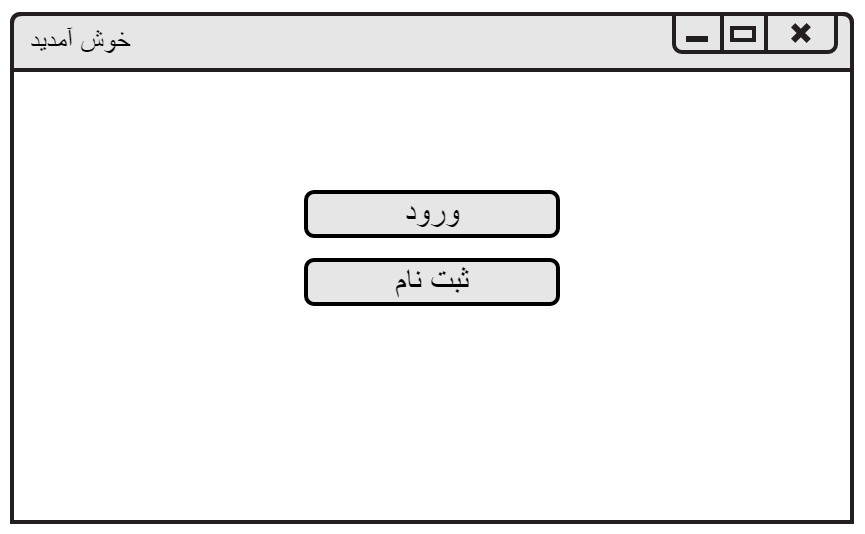
\includegraphics[width=0.5\textwidth]{Prototype/Accounting/HomePage.png}
\end{center}

\vspace{1cm}
صفحه‌ی ورود
\begin{center}
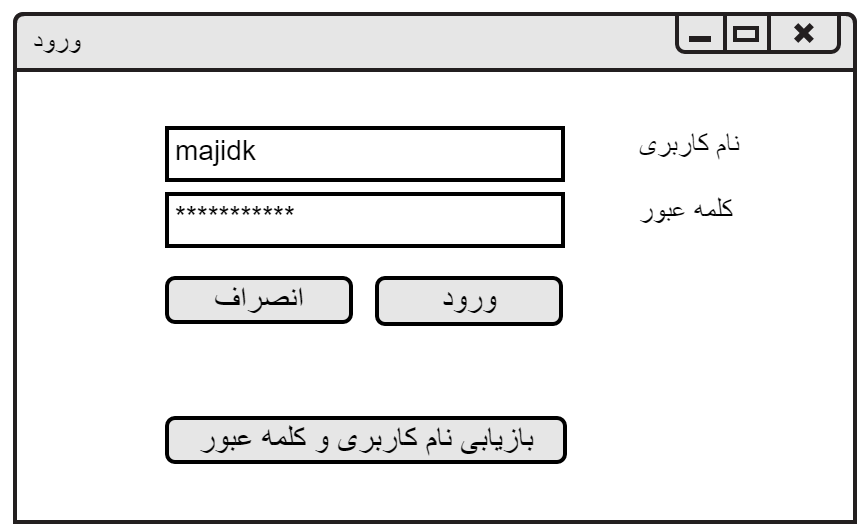
\includegraphics[width=0.5\textwidth]{Prototype/Accounting/Login.png}
\end{center}

\newpage
\vspace{1cm}
صفحه‌ی ثبت‌نام
\begin{center}
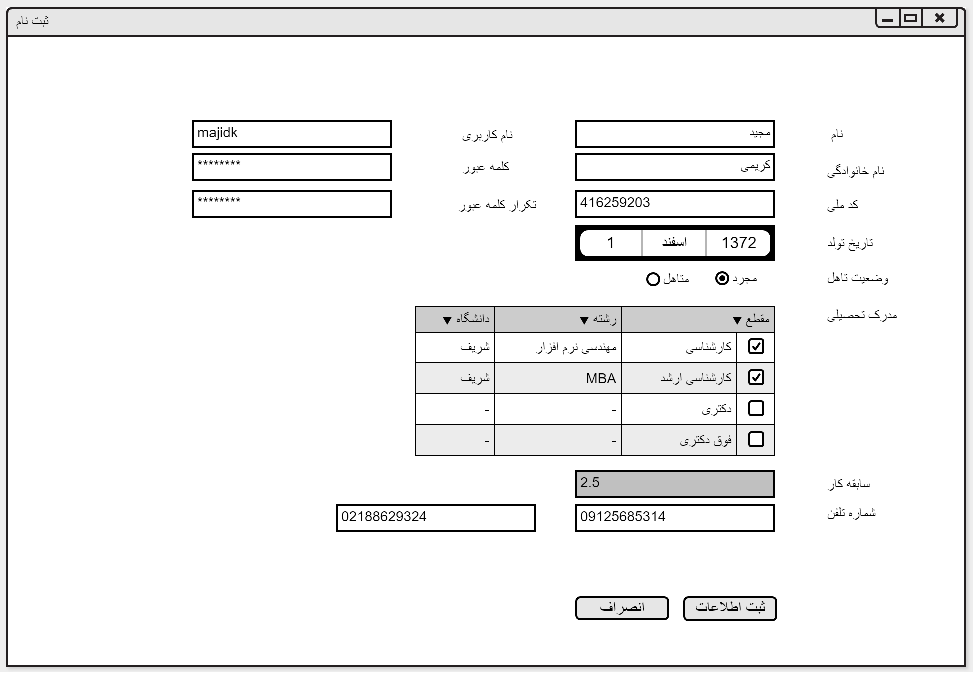
\includegraphics[width=\textwidth]{Prototype/Accounting/Register.png}
\end{center}

\vspace{1cm}
صفحه‌ی تغییر رمز عبور
\begin{center}
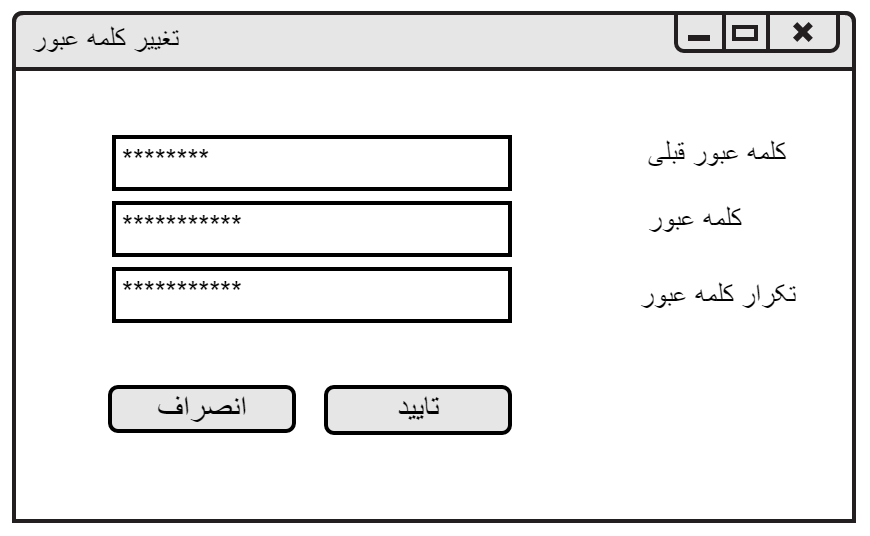
\includegraphics[width=0.5\textwidth]{Prototype/Accounting/ChangePassword.png}
\end{center}

\newpage
\vspace{1cm}
صفحه‌ی اطلاعات شخصی 
\begin{center}
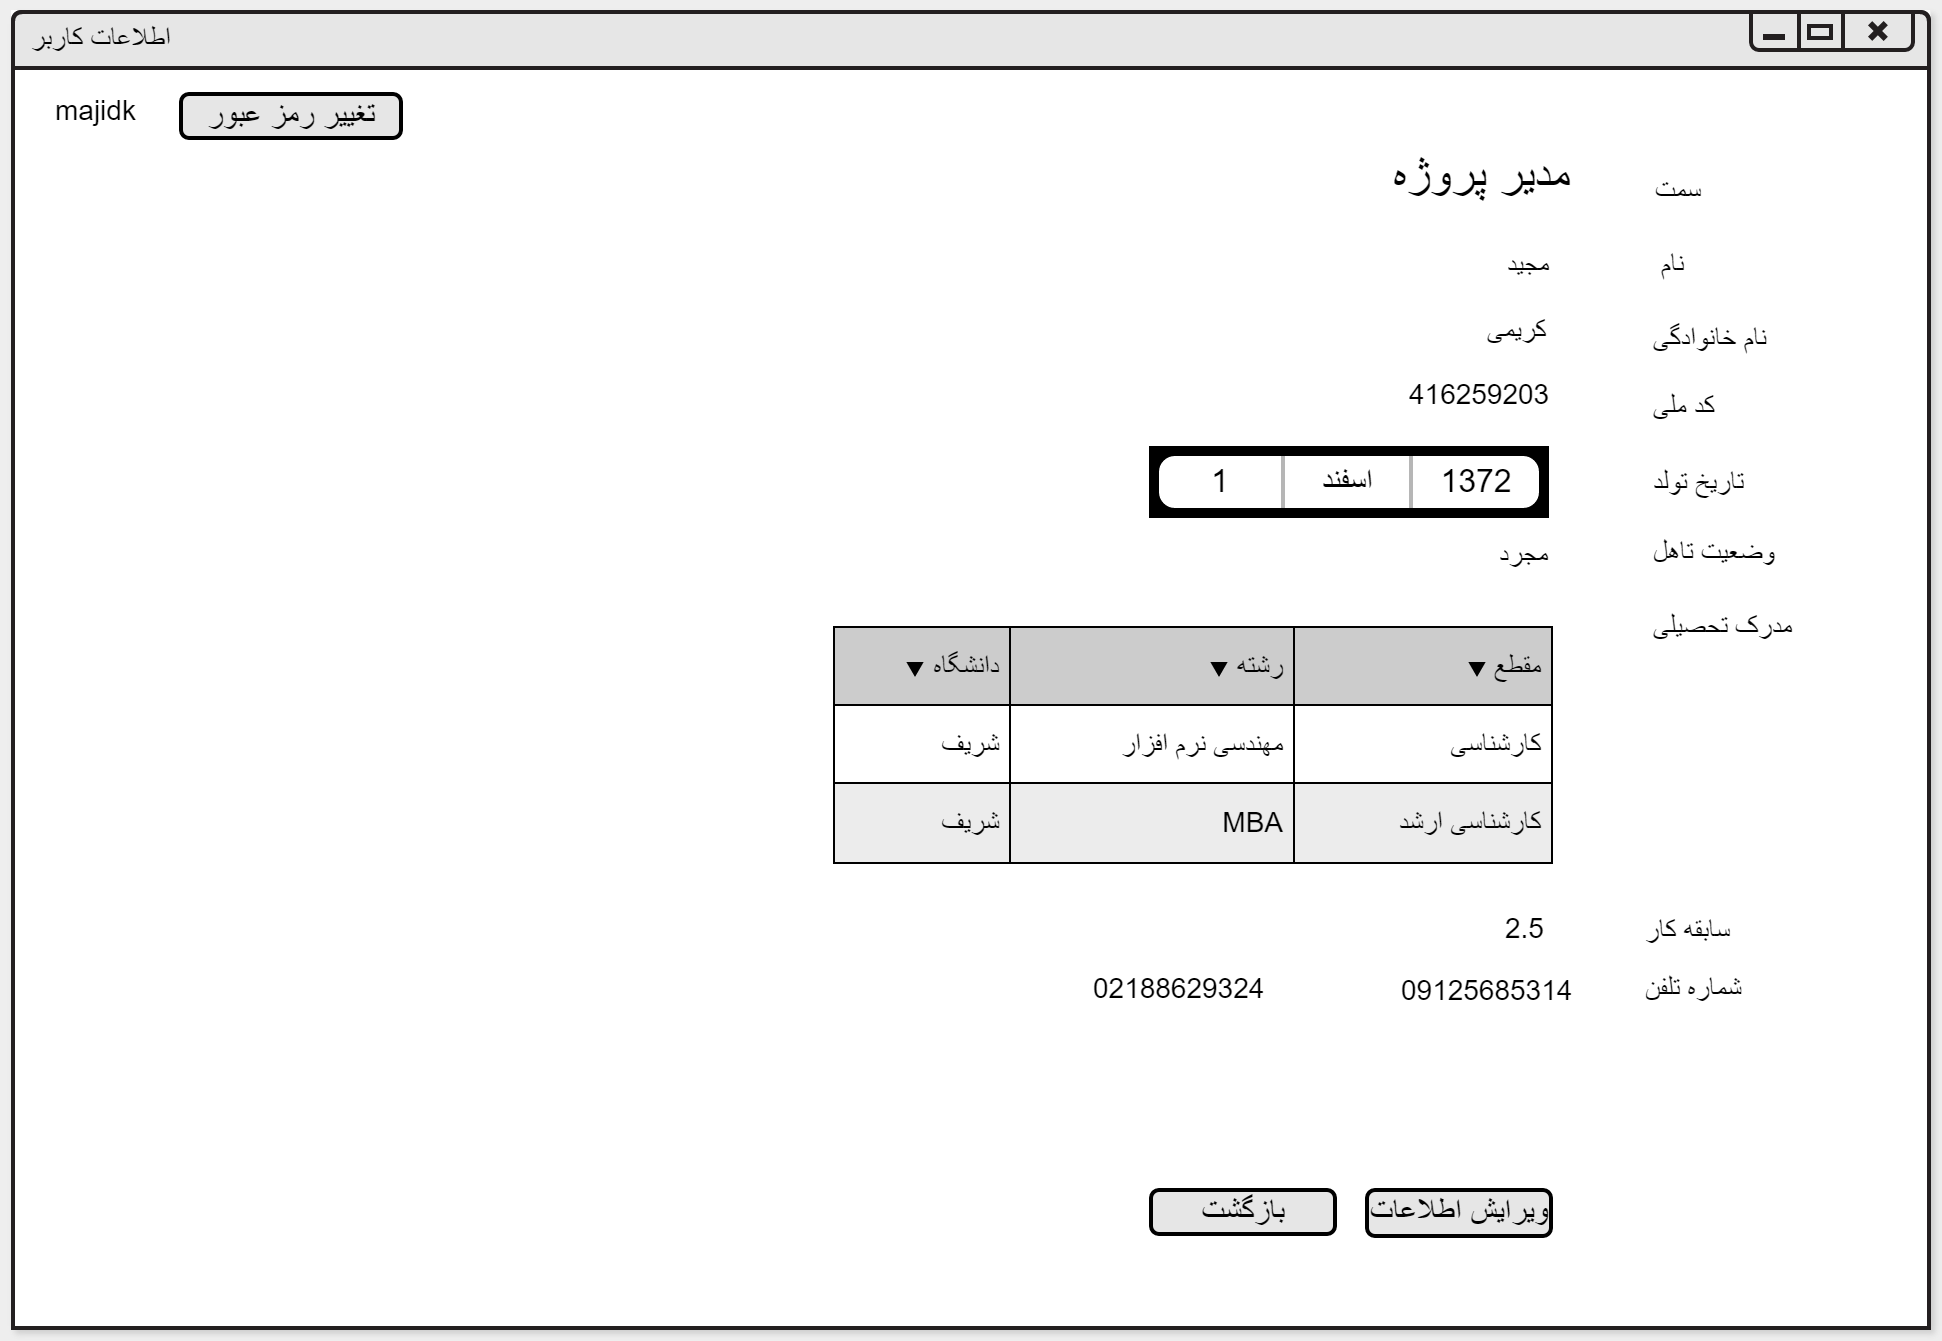
\includegraphics[width=\textwidth]{Prototype/Accounting/PersonalInformation.png}
\end{center}

\vspace{1cm}
صفحه‌ی ویرایش اطلاعات شخصی 
\begin{center}
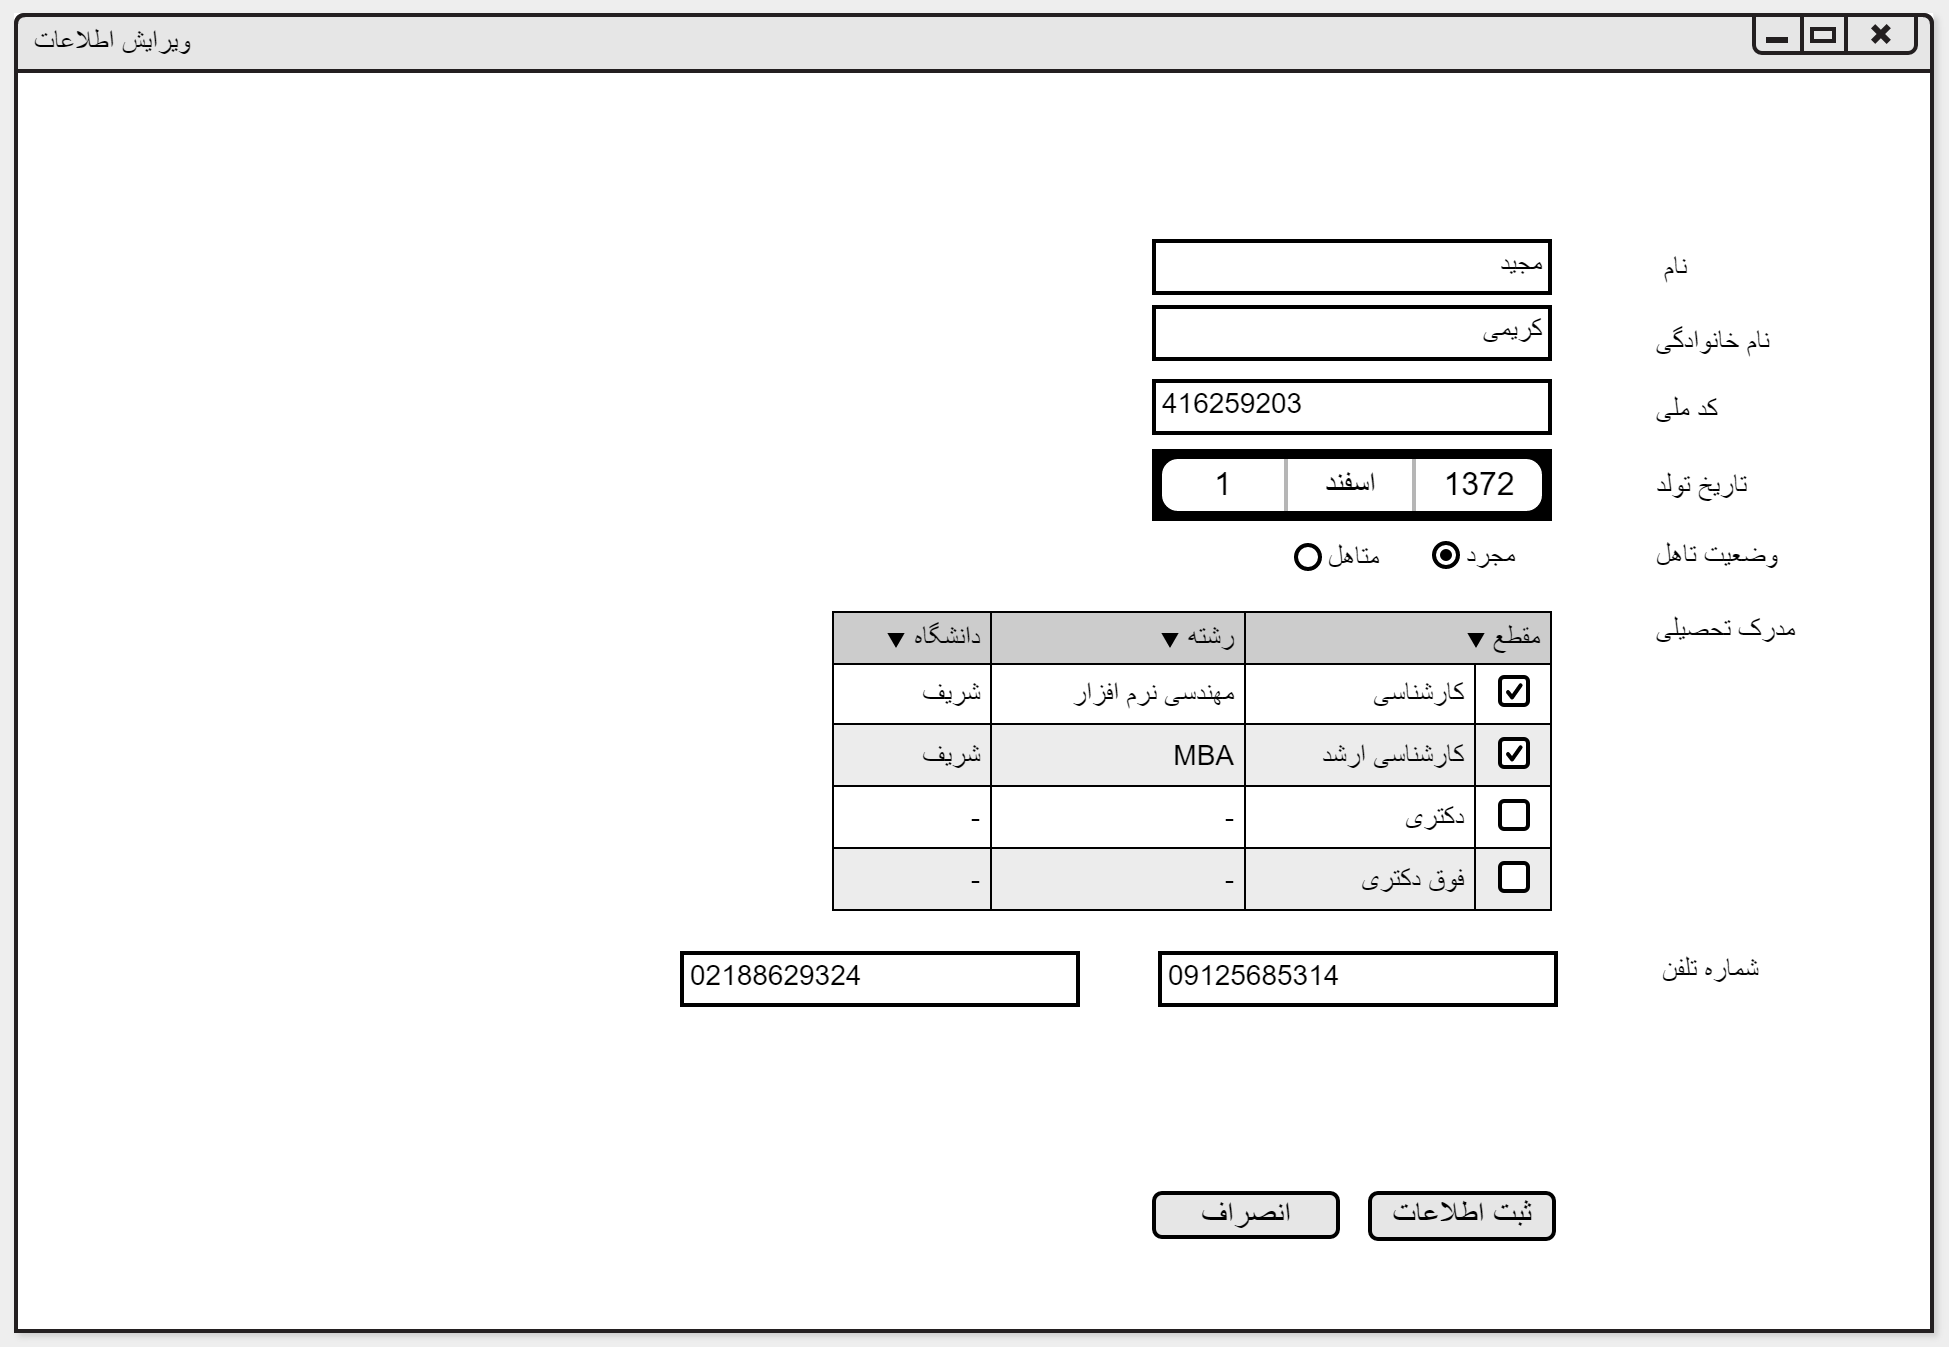
\includegraphics[width=\textwidth]{Prototype/Accounting/EditPersonalInformation.png}
\end{center}

\newpage
\subsection{صفحات کارمند}

\vspace{1cm}
صفحه‌ی پنل اصلی کارمند
\begin{center}
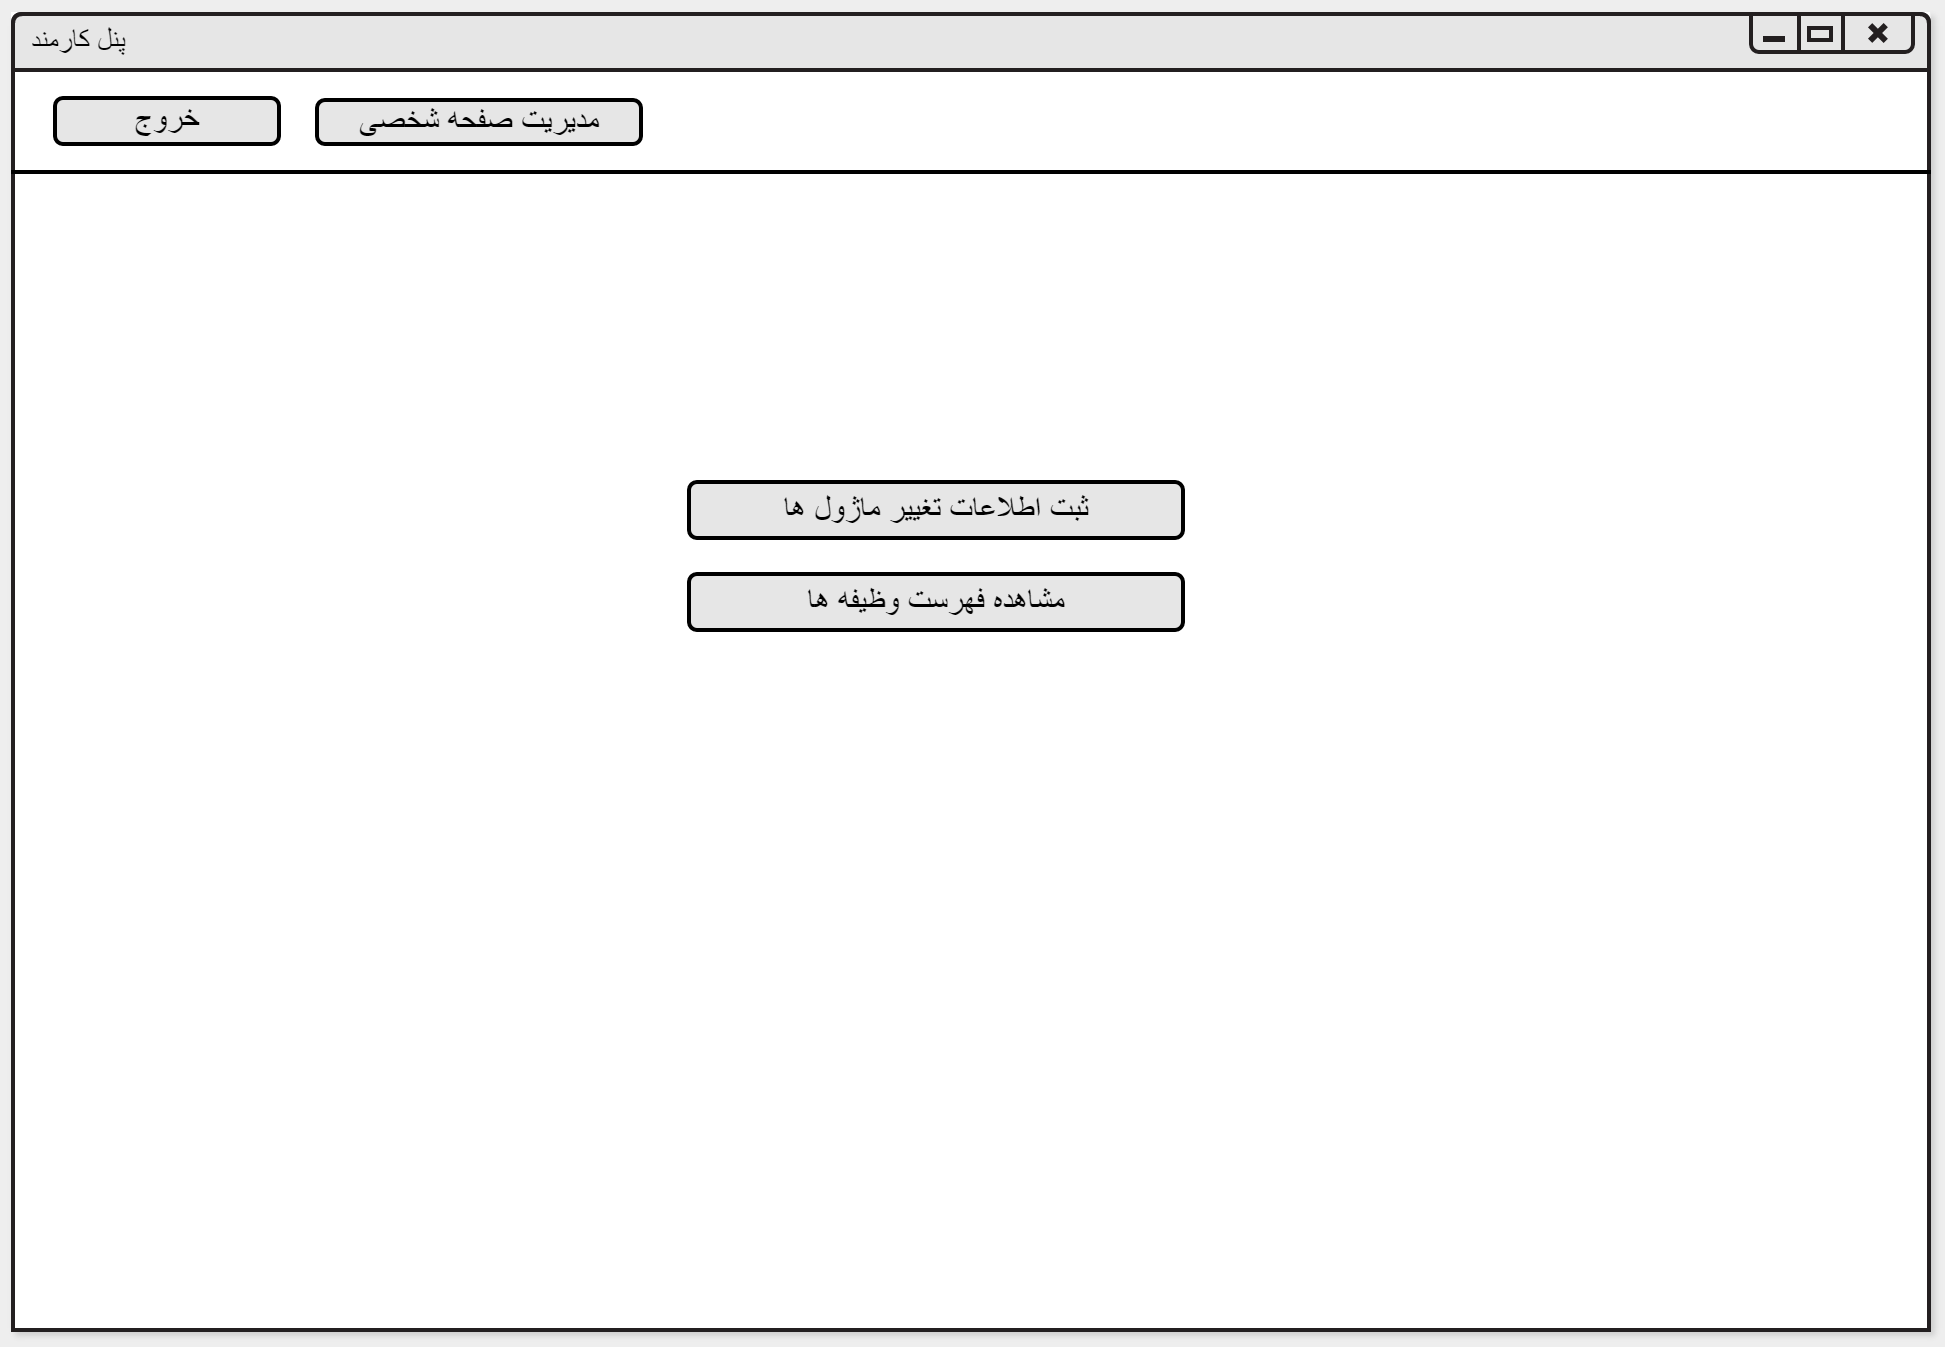
\includegraphics[width=\textwidth]{Prototype/Employee/EmployeePanel.png}
\end{center}

\newpage
\vspace{1cm}
صفحه‌ی فهرست ماژول‌های قابل دسترسی
\begin{center}
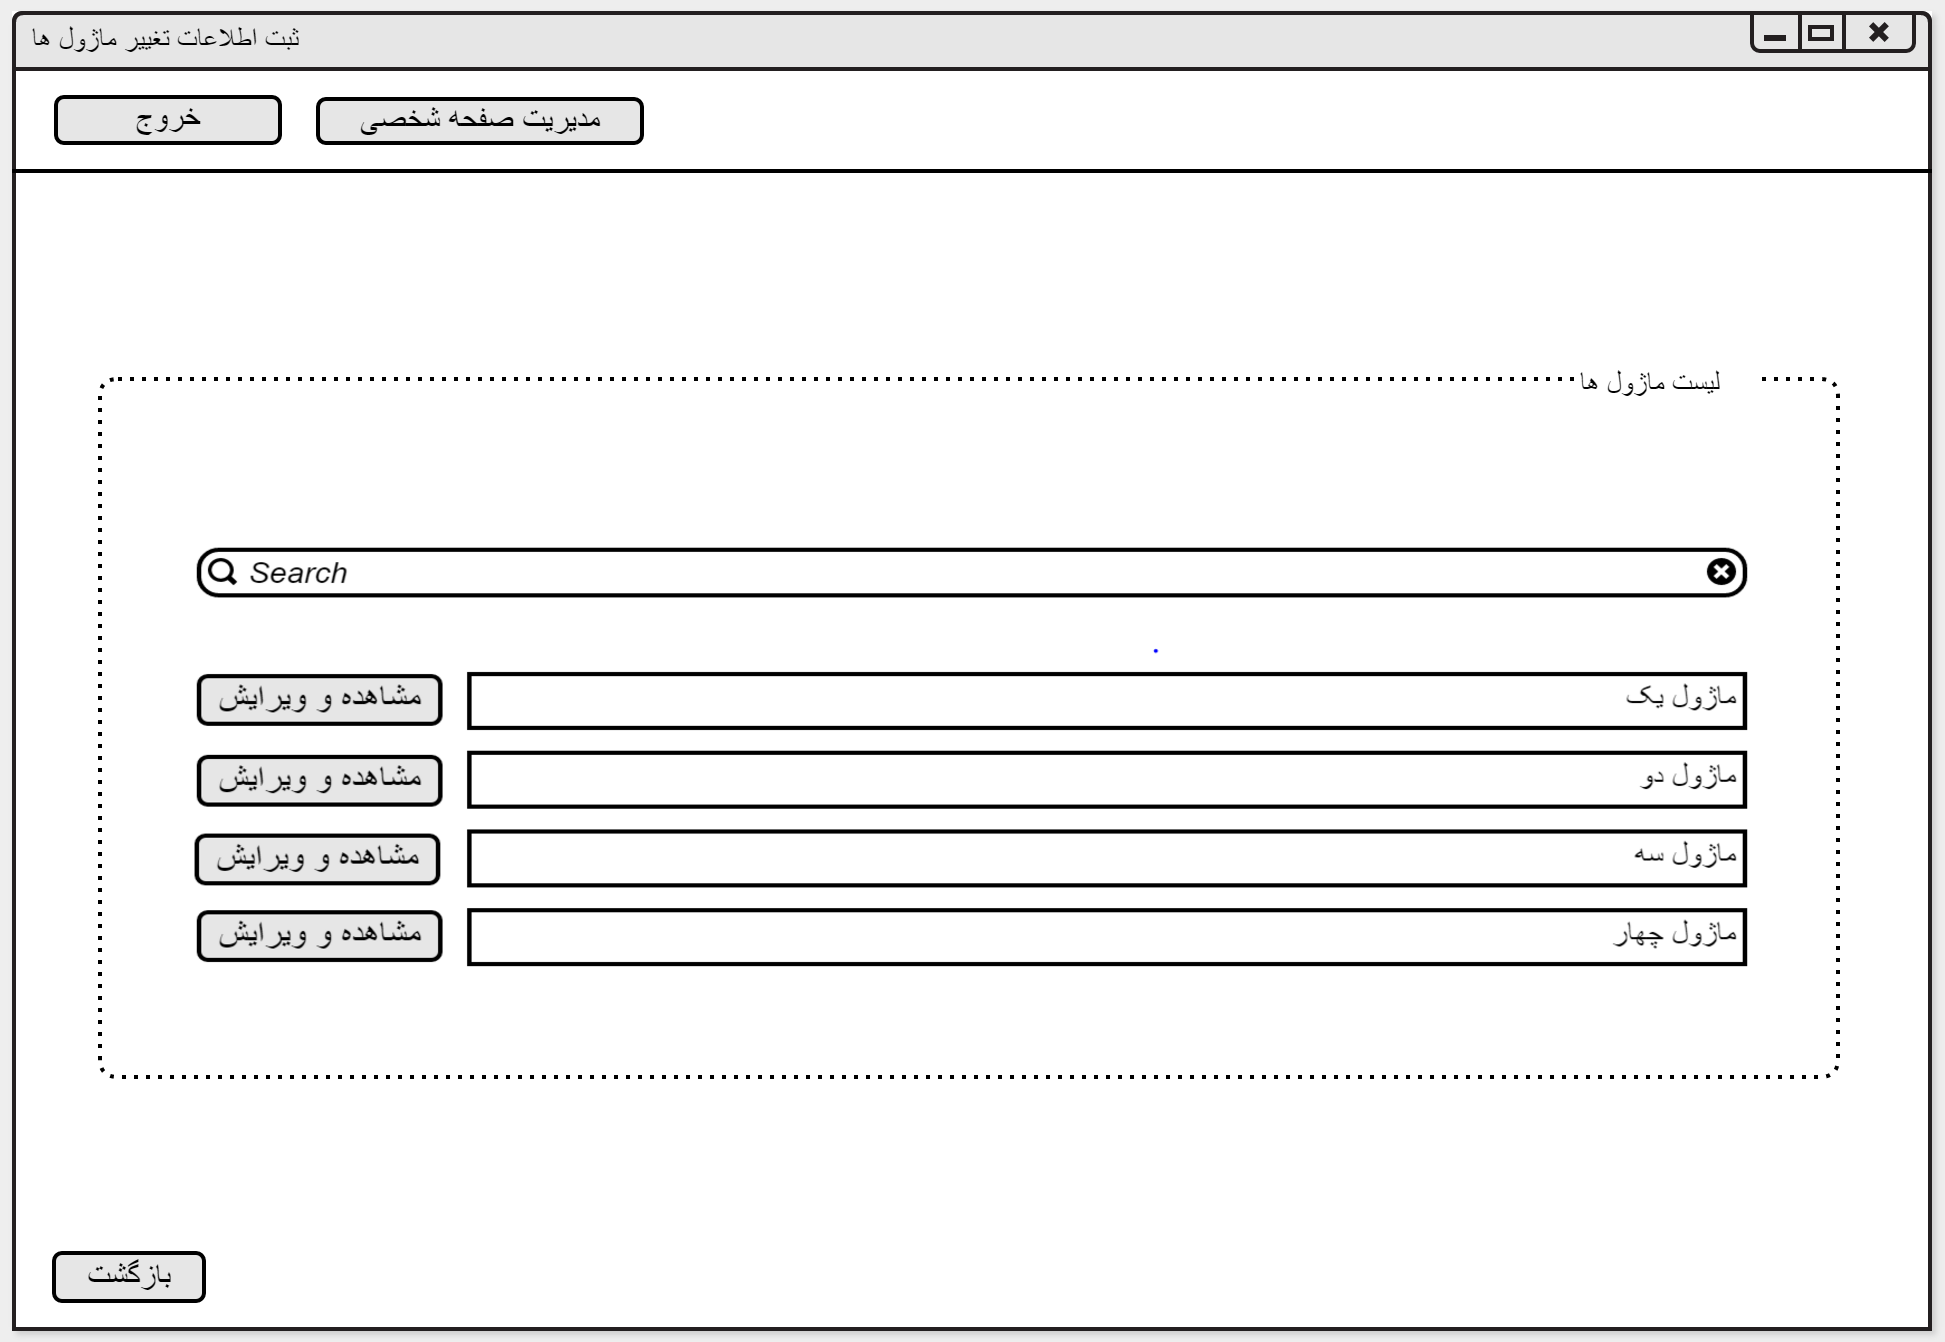
\includegraphics[width=\textwidth]{Prototype/Employee/ChangeModuleInformation.png}
\end{center}

\vspace{1cm}
صفحه‌ی ثبت اطلاعات تغییر یک ماژول
\begin{center}
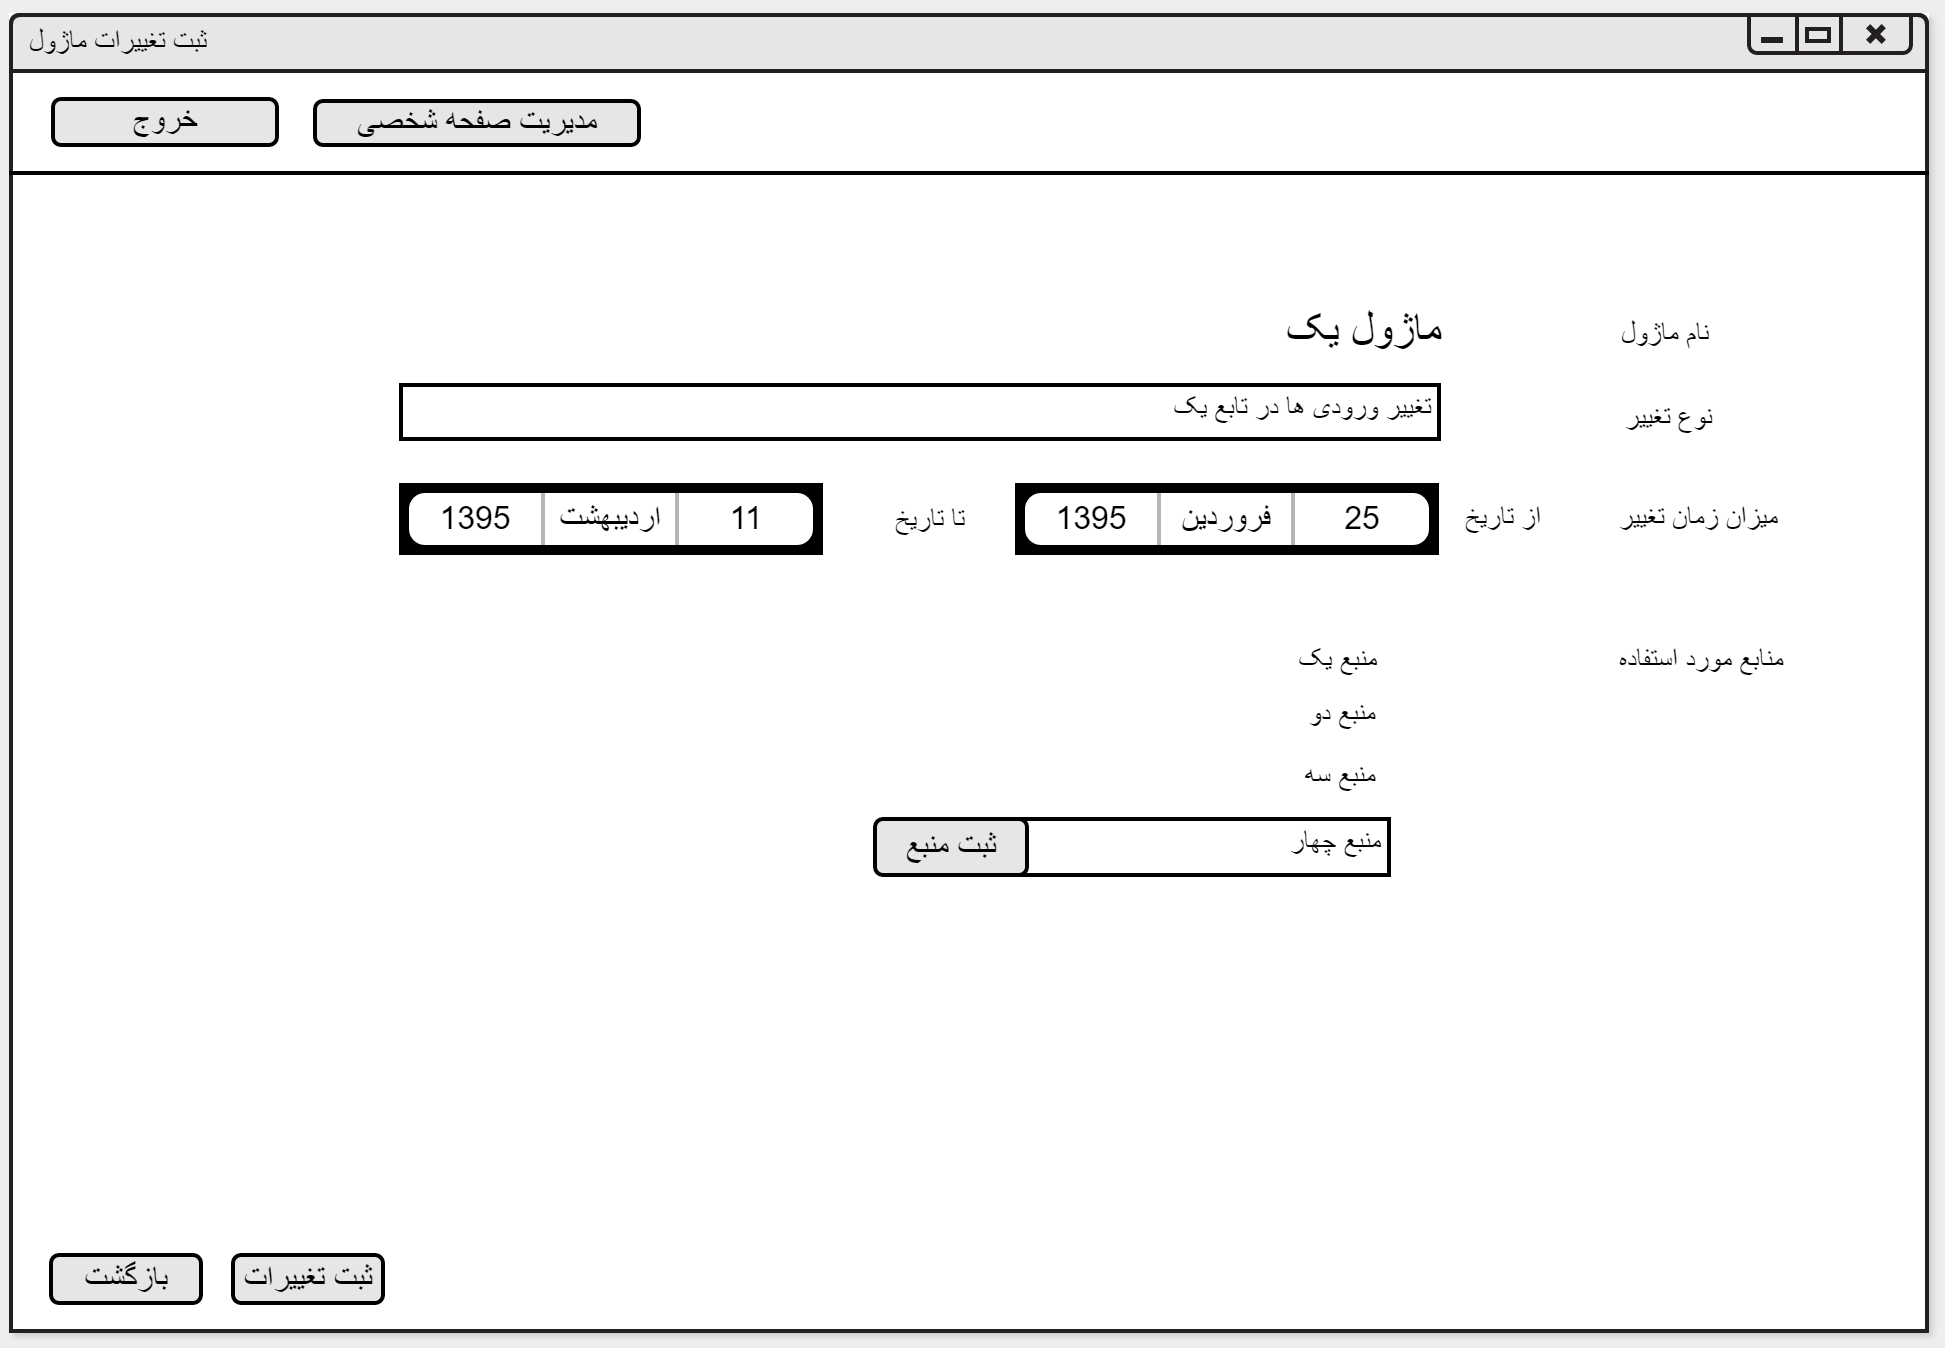
\includegraphics[width=\textwidth]{Prototype/Employee/ChangeOneModule.png}
\end{center}

\newpage
\vspace{1cm}
صفحه‌ی فهرست وظیفه‌ها
\begin{center}
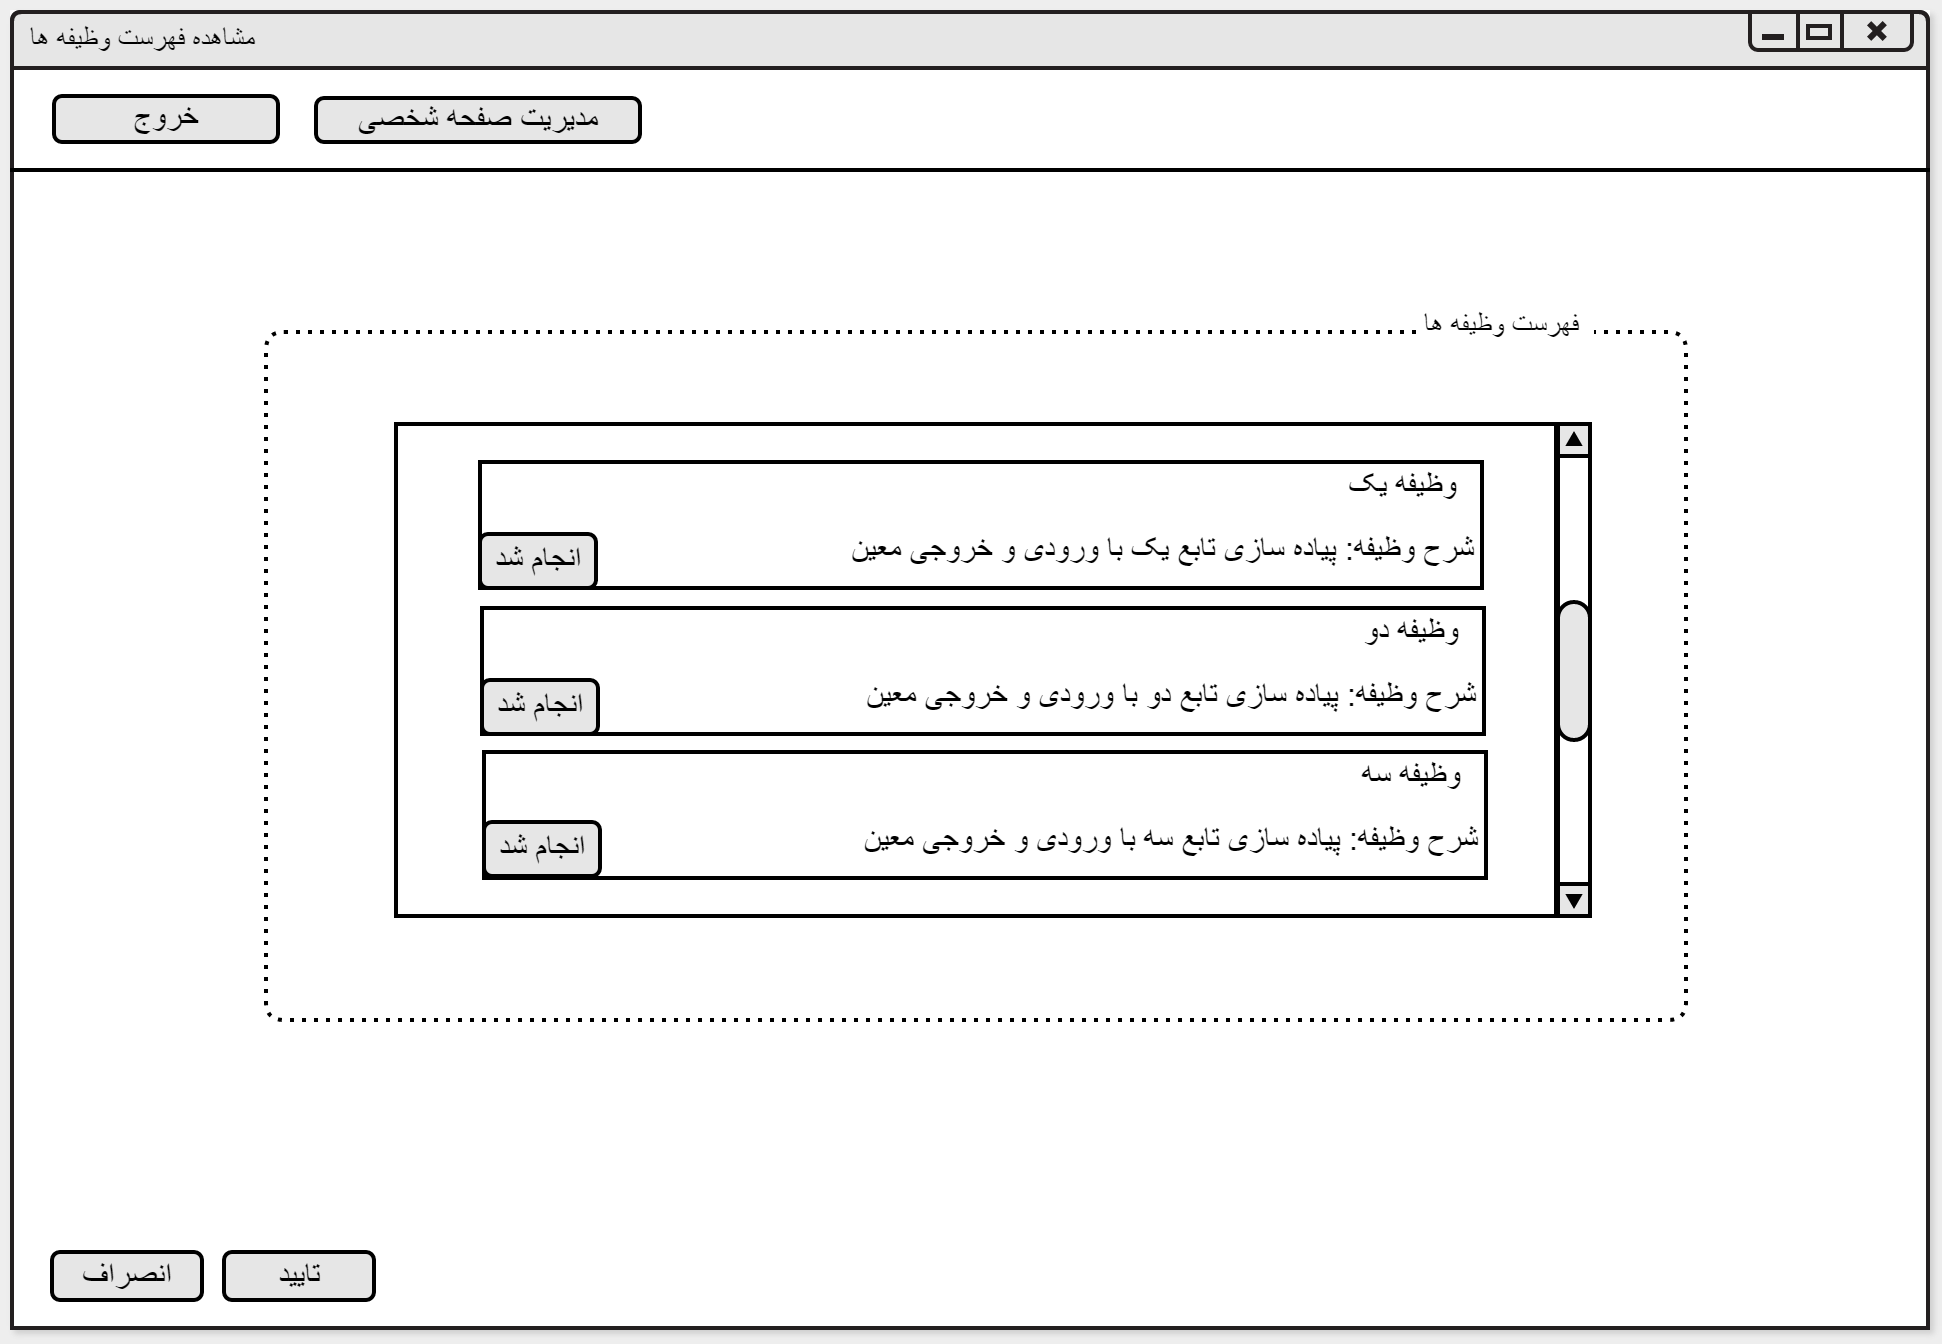
\includegraphics[width=\textwidth]{Prototype/Employee/TasksList.png}
\end{center}

\newpage
\subsection{صفحات مدیریت پروژه}

\vspace{1cm}
صفحه‌ی فهرست پروژه‌های قابل دسترسی
\begin{center}
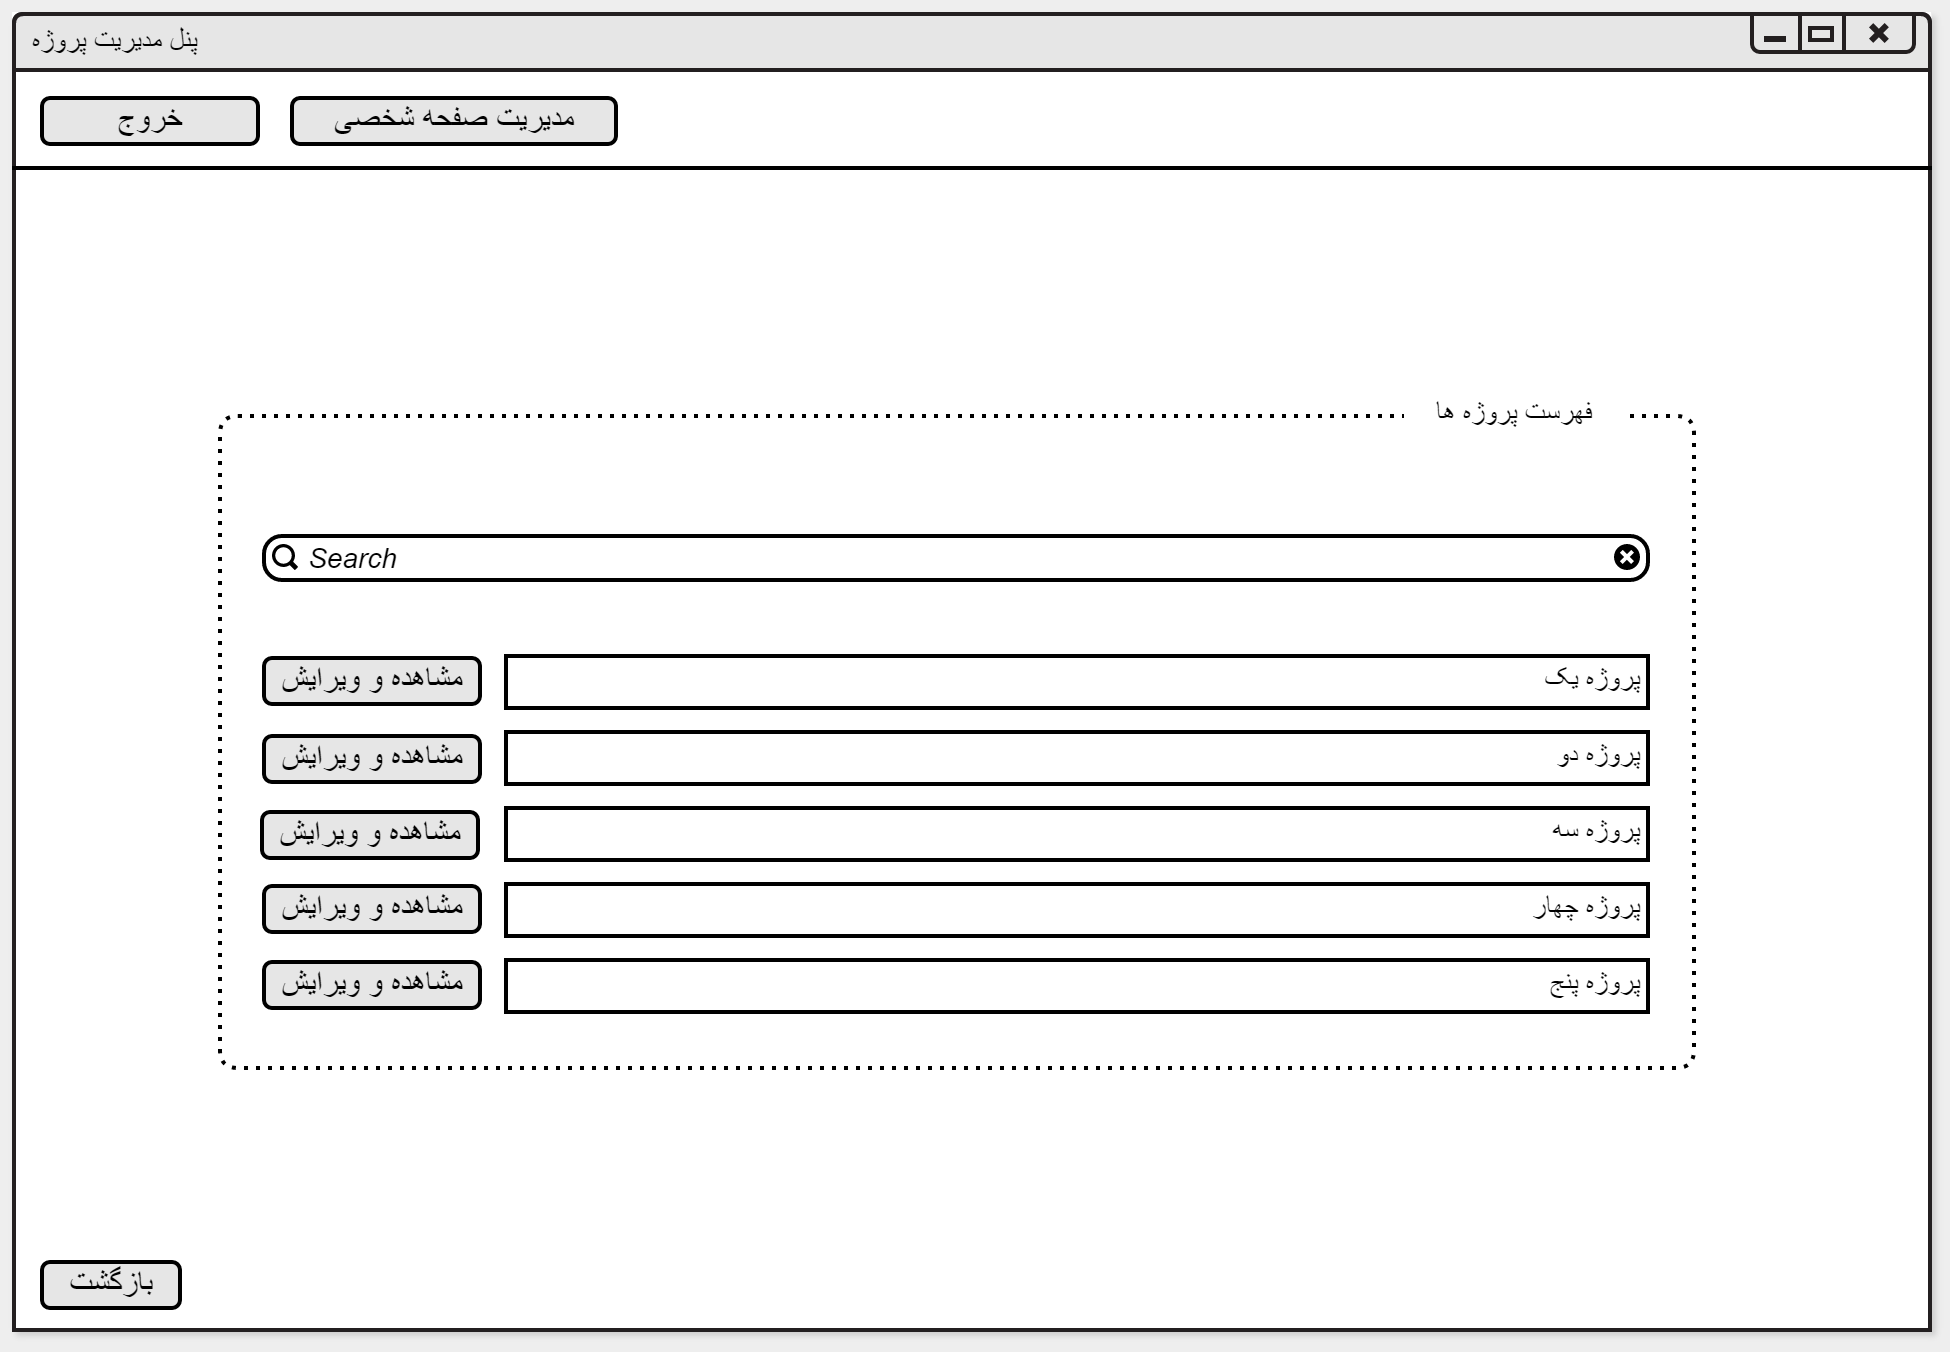
\includegraphics[width=\textwidth]{Prototype/ProjectManager/ProjectsList.png}
\end{center}

\newpage
\vspace{1cm}
صفحه‌ی پنل اصلی مدیریت یک پروژه
\begin{center}
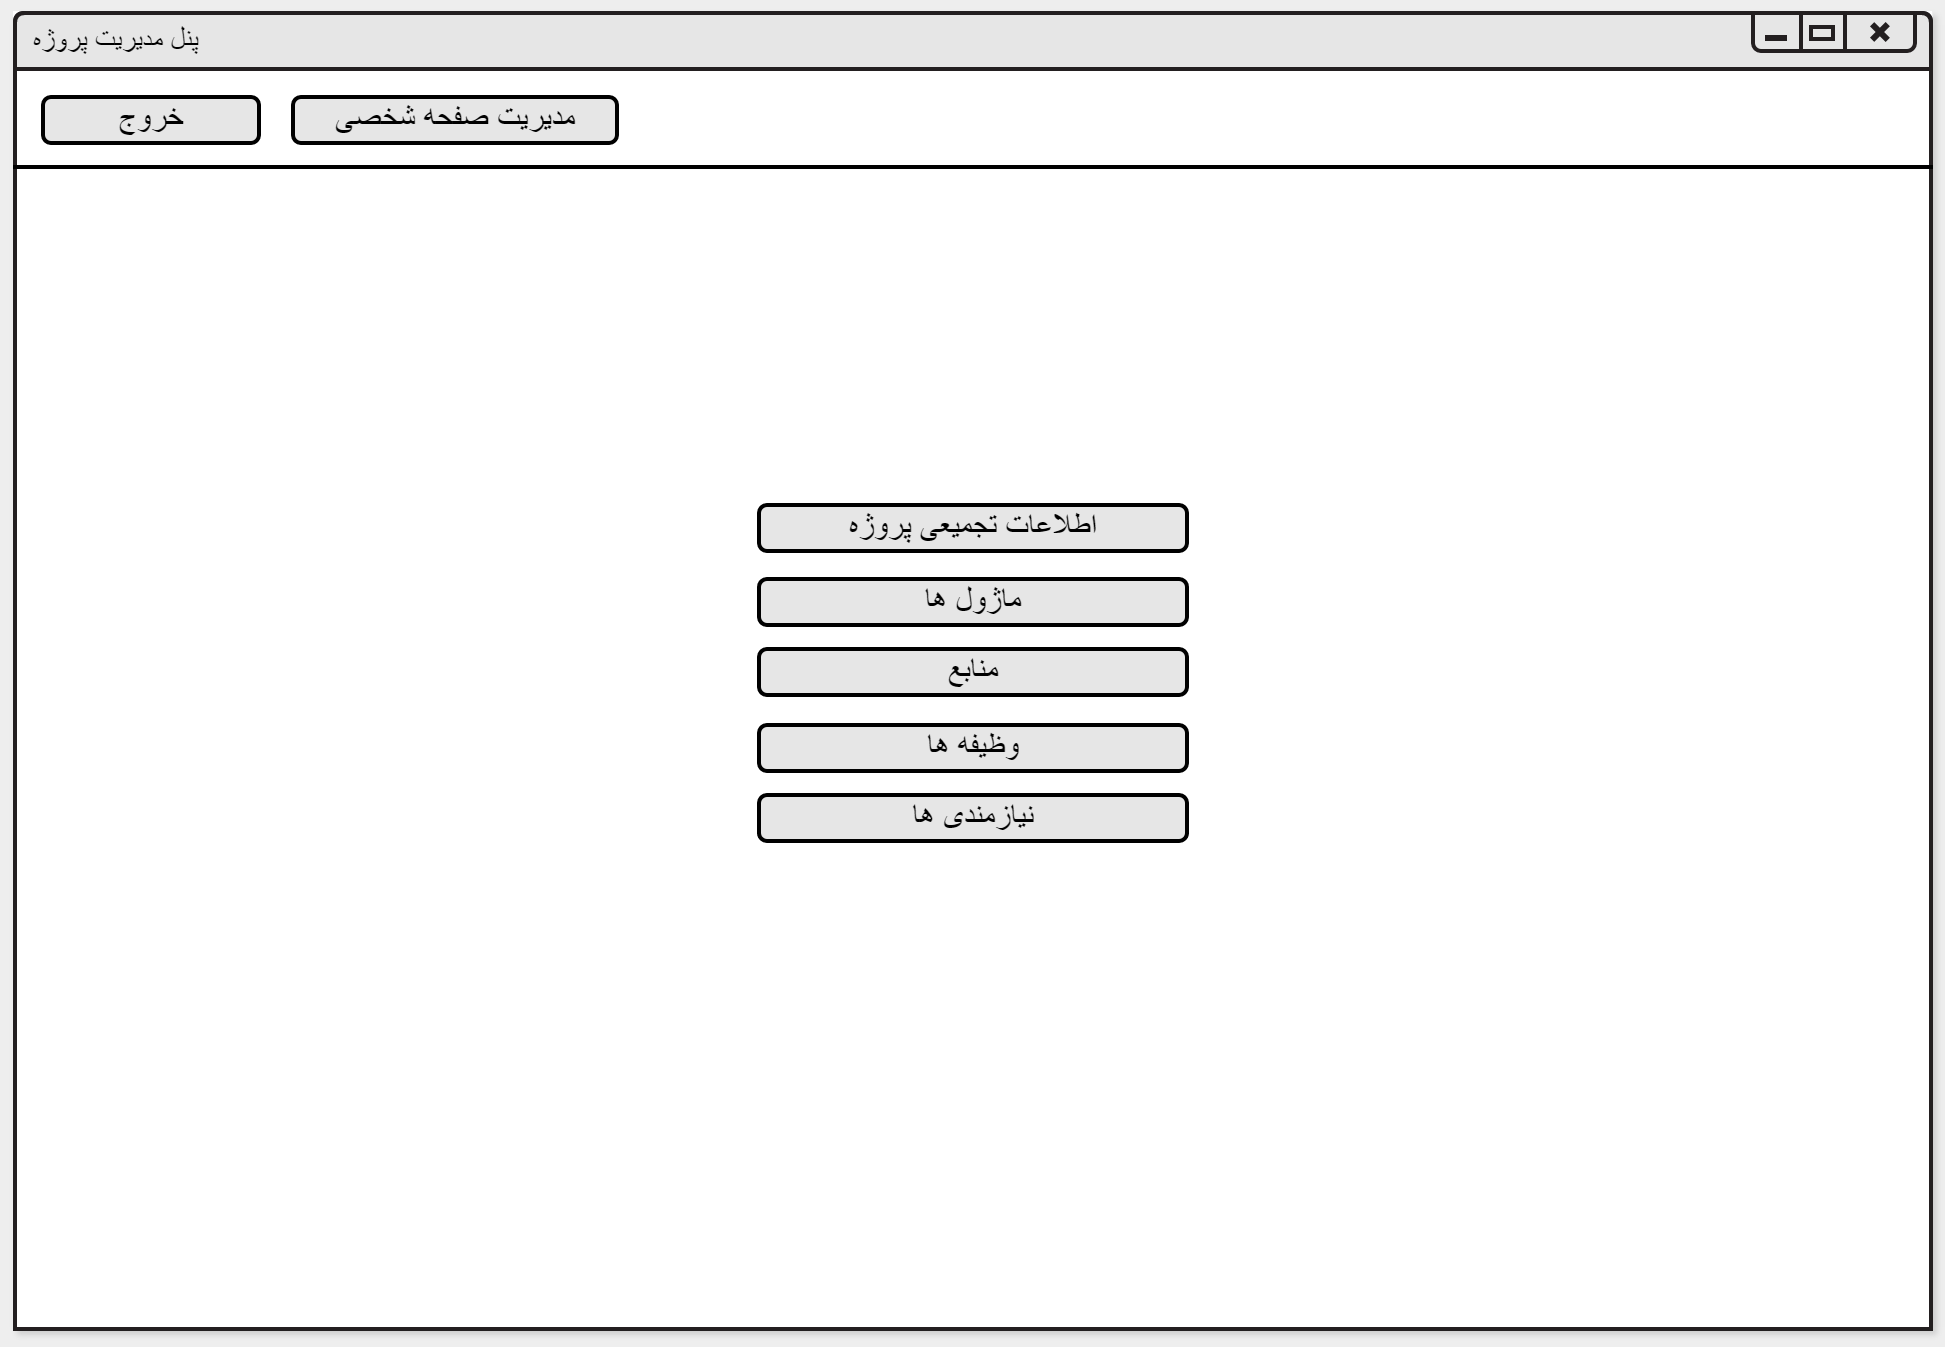
\includegraphics[width=\textwidth]{Prototype/ProjectManager/ProjectManagementMainPanel.png}
\end{center}

\vspace{1cm}
صفحه‌ی اطلاعات تجمیعی پروژه
\begin{center}
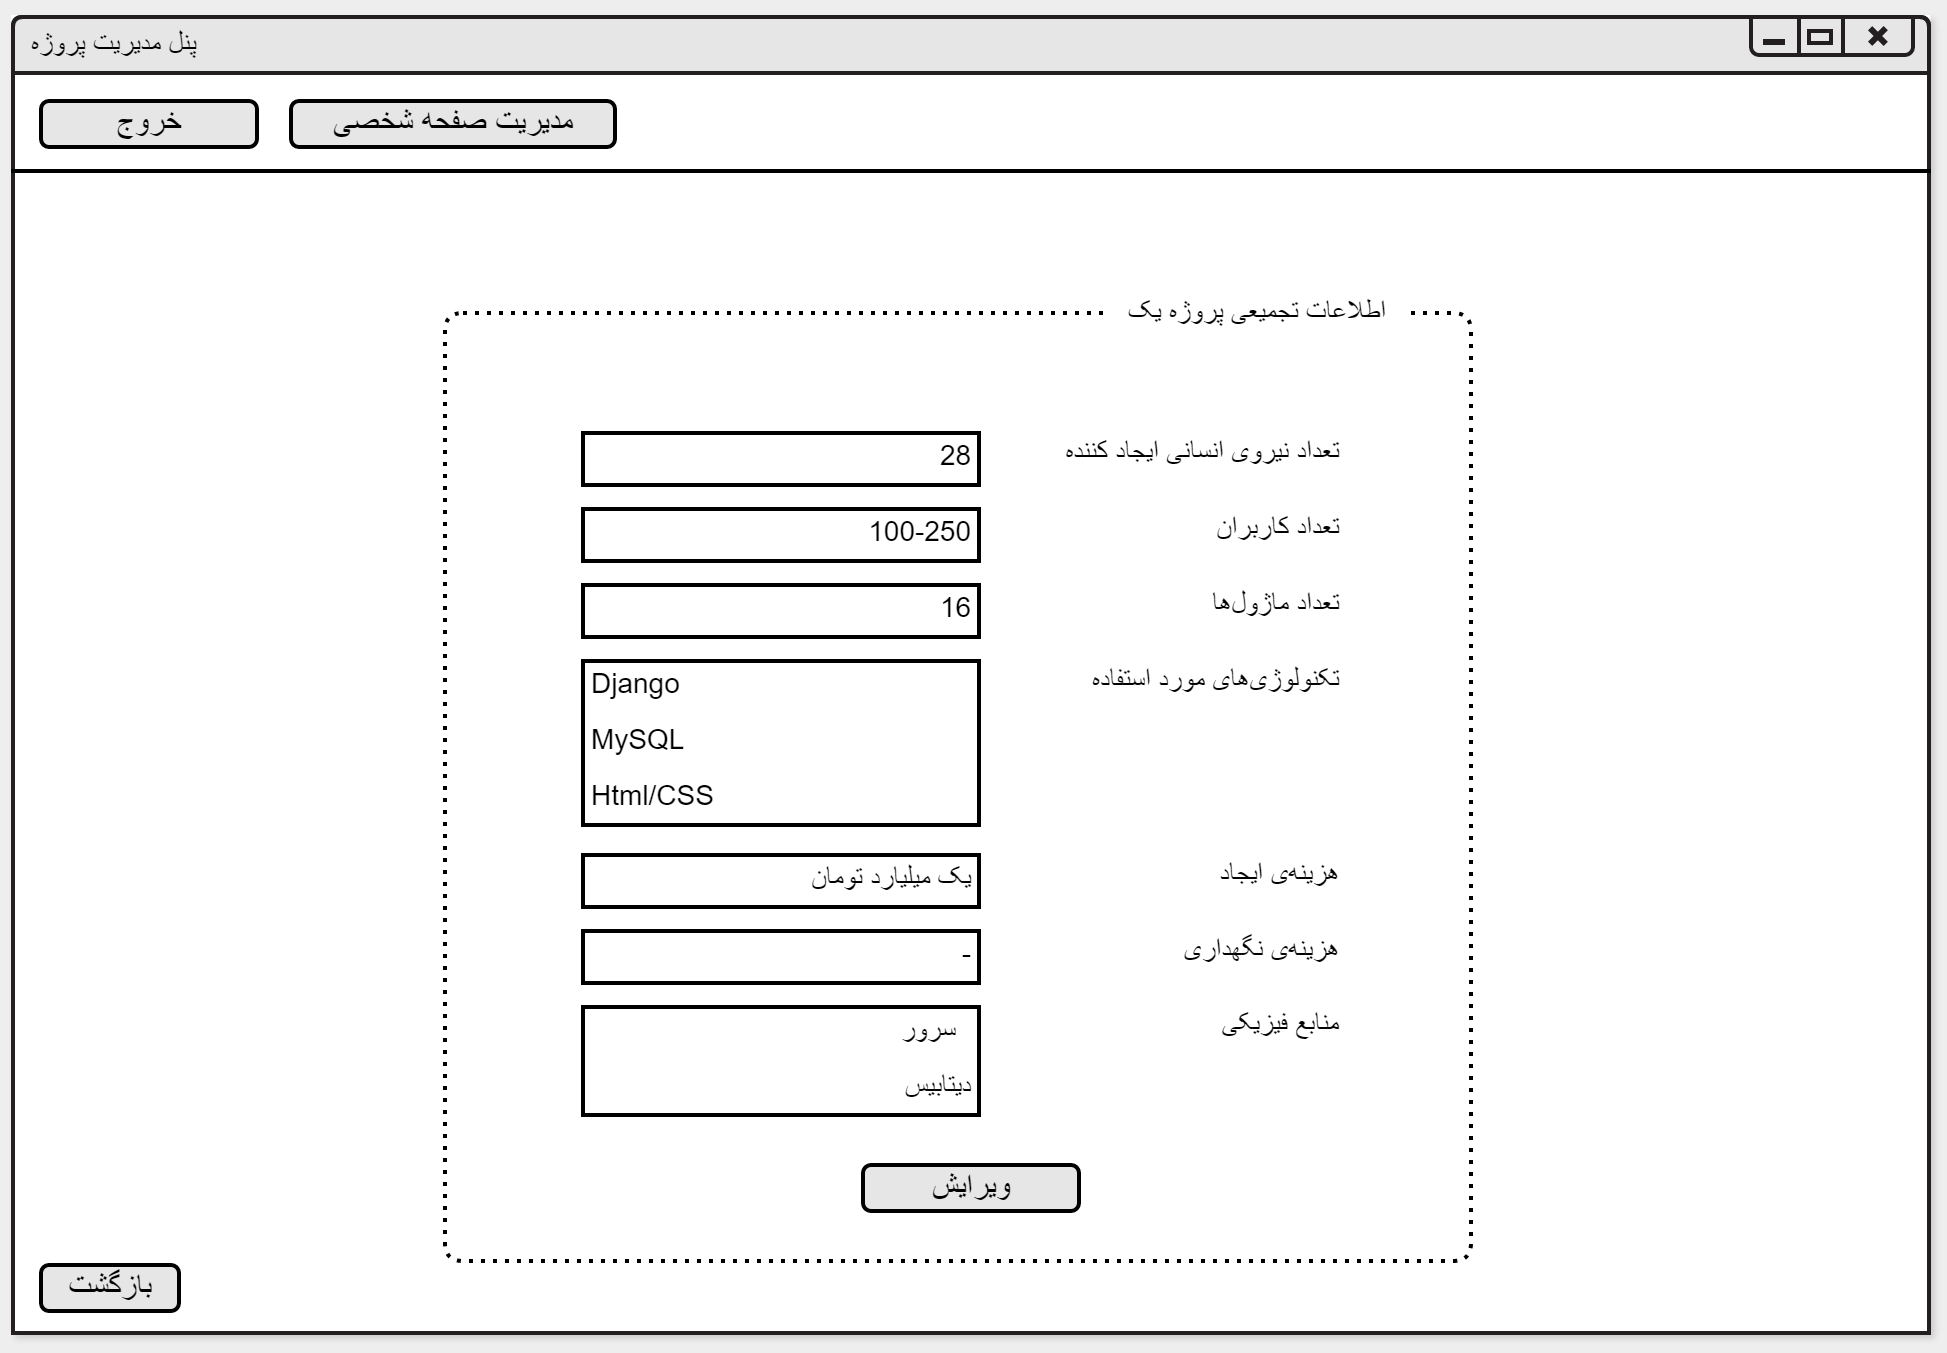
\includegraphics[width=\textwidth]{Prototype/ProjectManager/ProjectInformation.png}
\end{center}

\newpage
\vspace{1cm}
صفحه‌ی فهرست ماژول‌های پروژه
\begin{center}
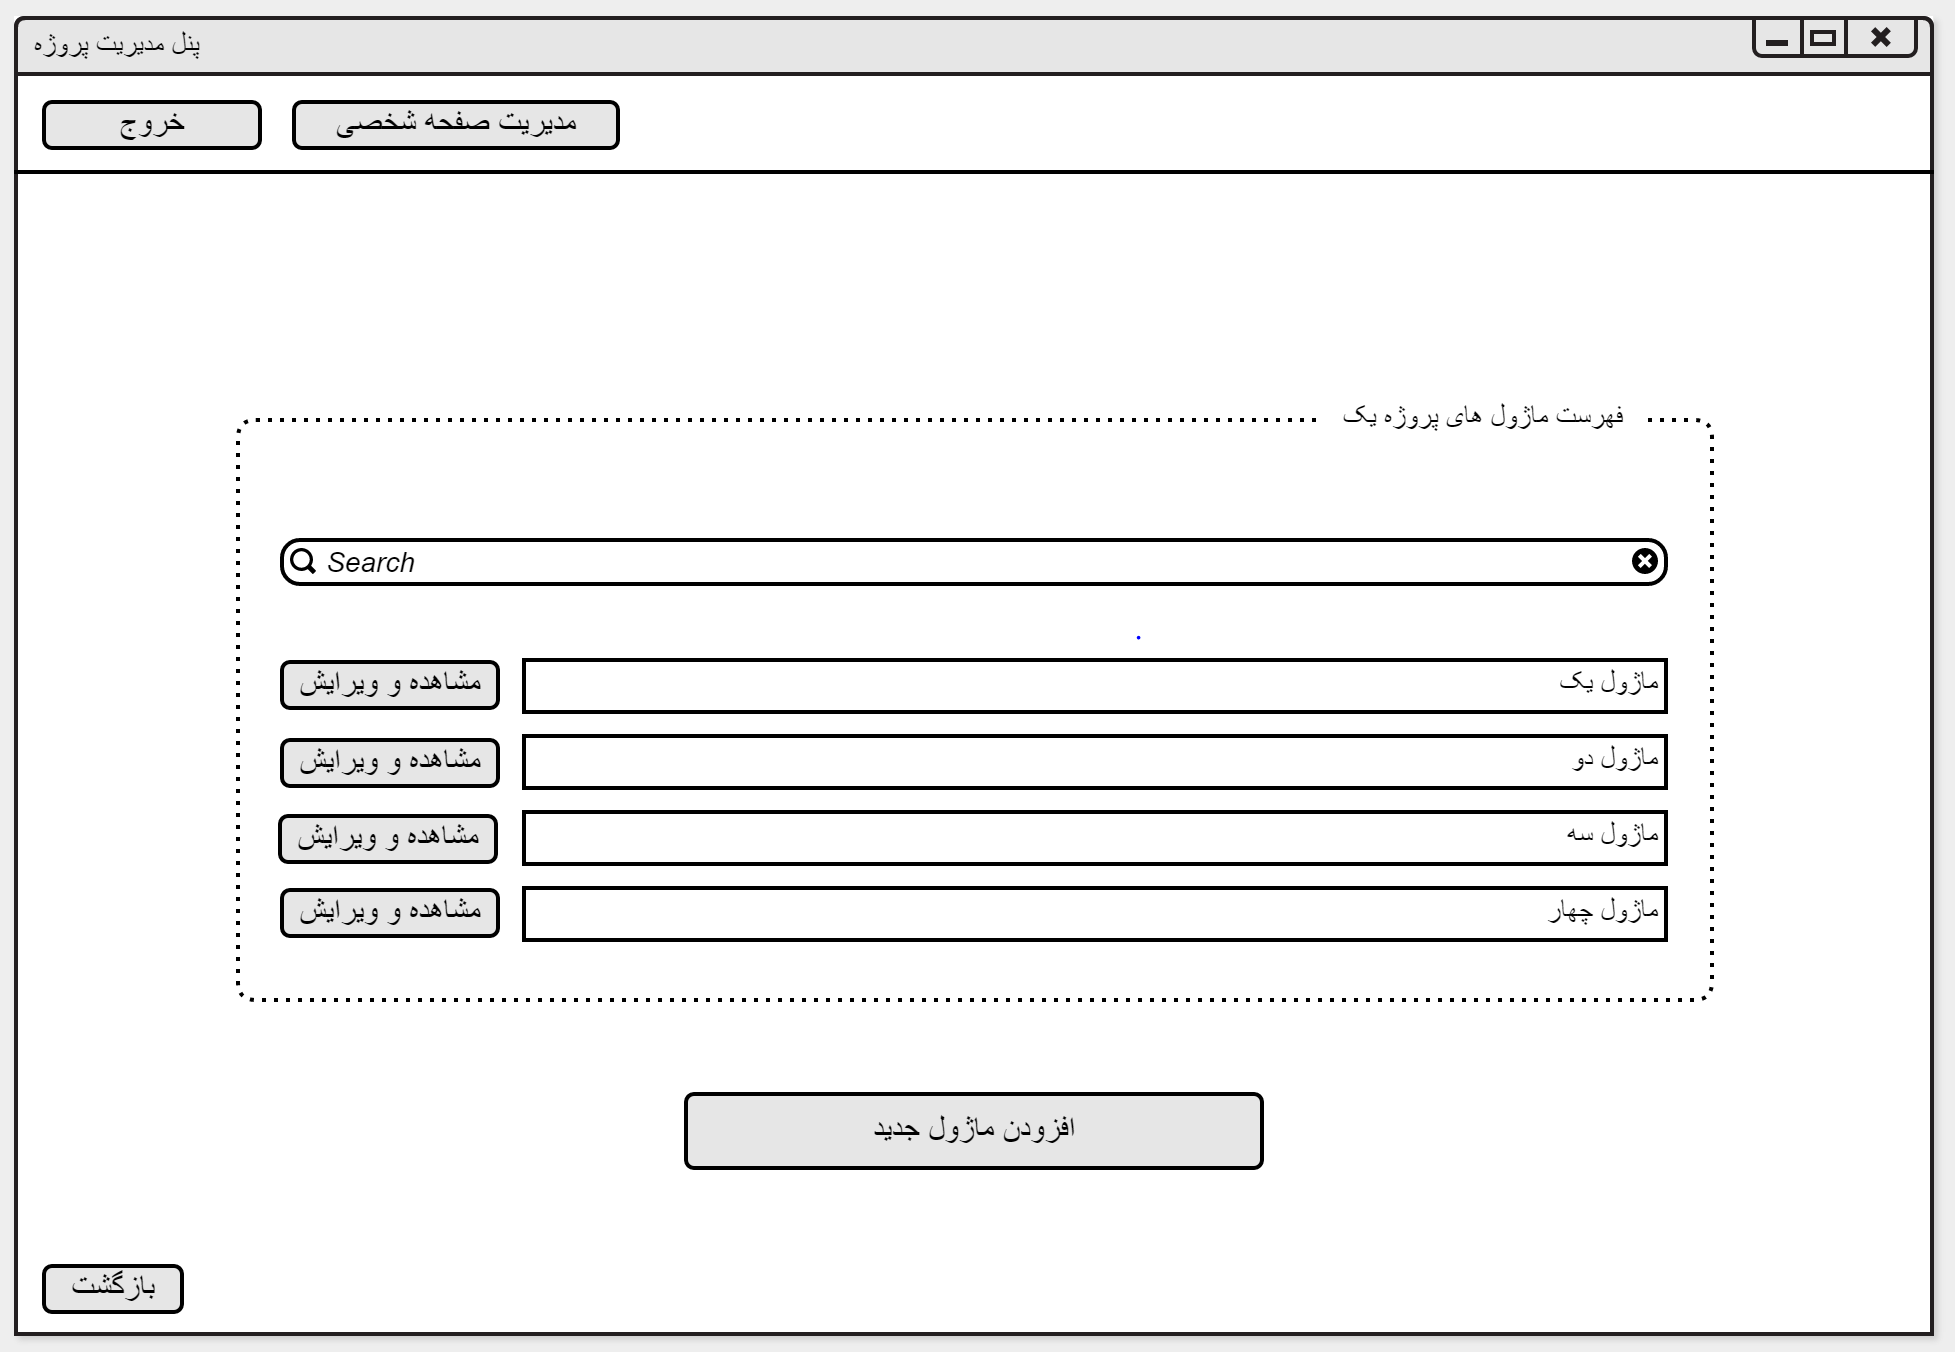
\includegraphics[width=\textwidth]{Prototype/ProjectManager/ProjectModulesList.png}
\end{center}

\vspace{1cm}
صفحه‌ی اطلاعات یک ماژول از پروژه 
\begin{center}
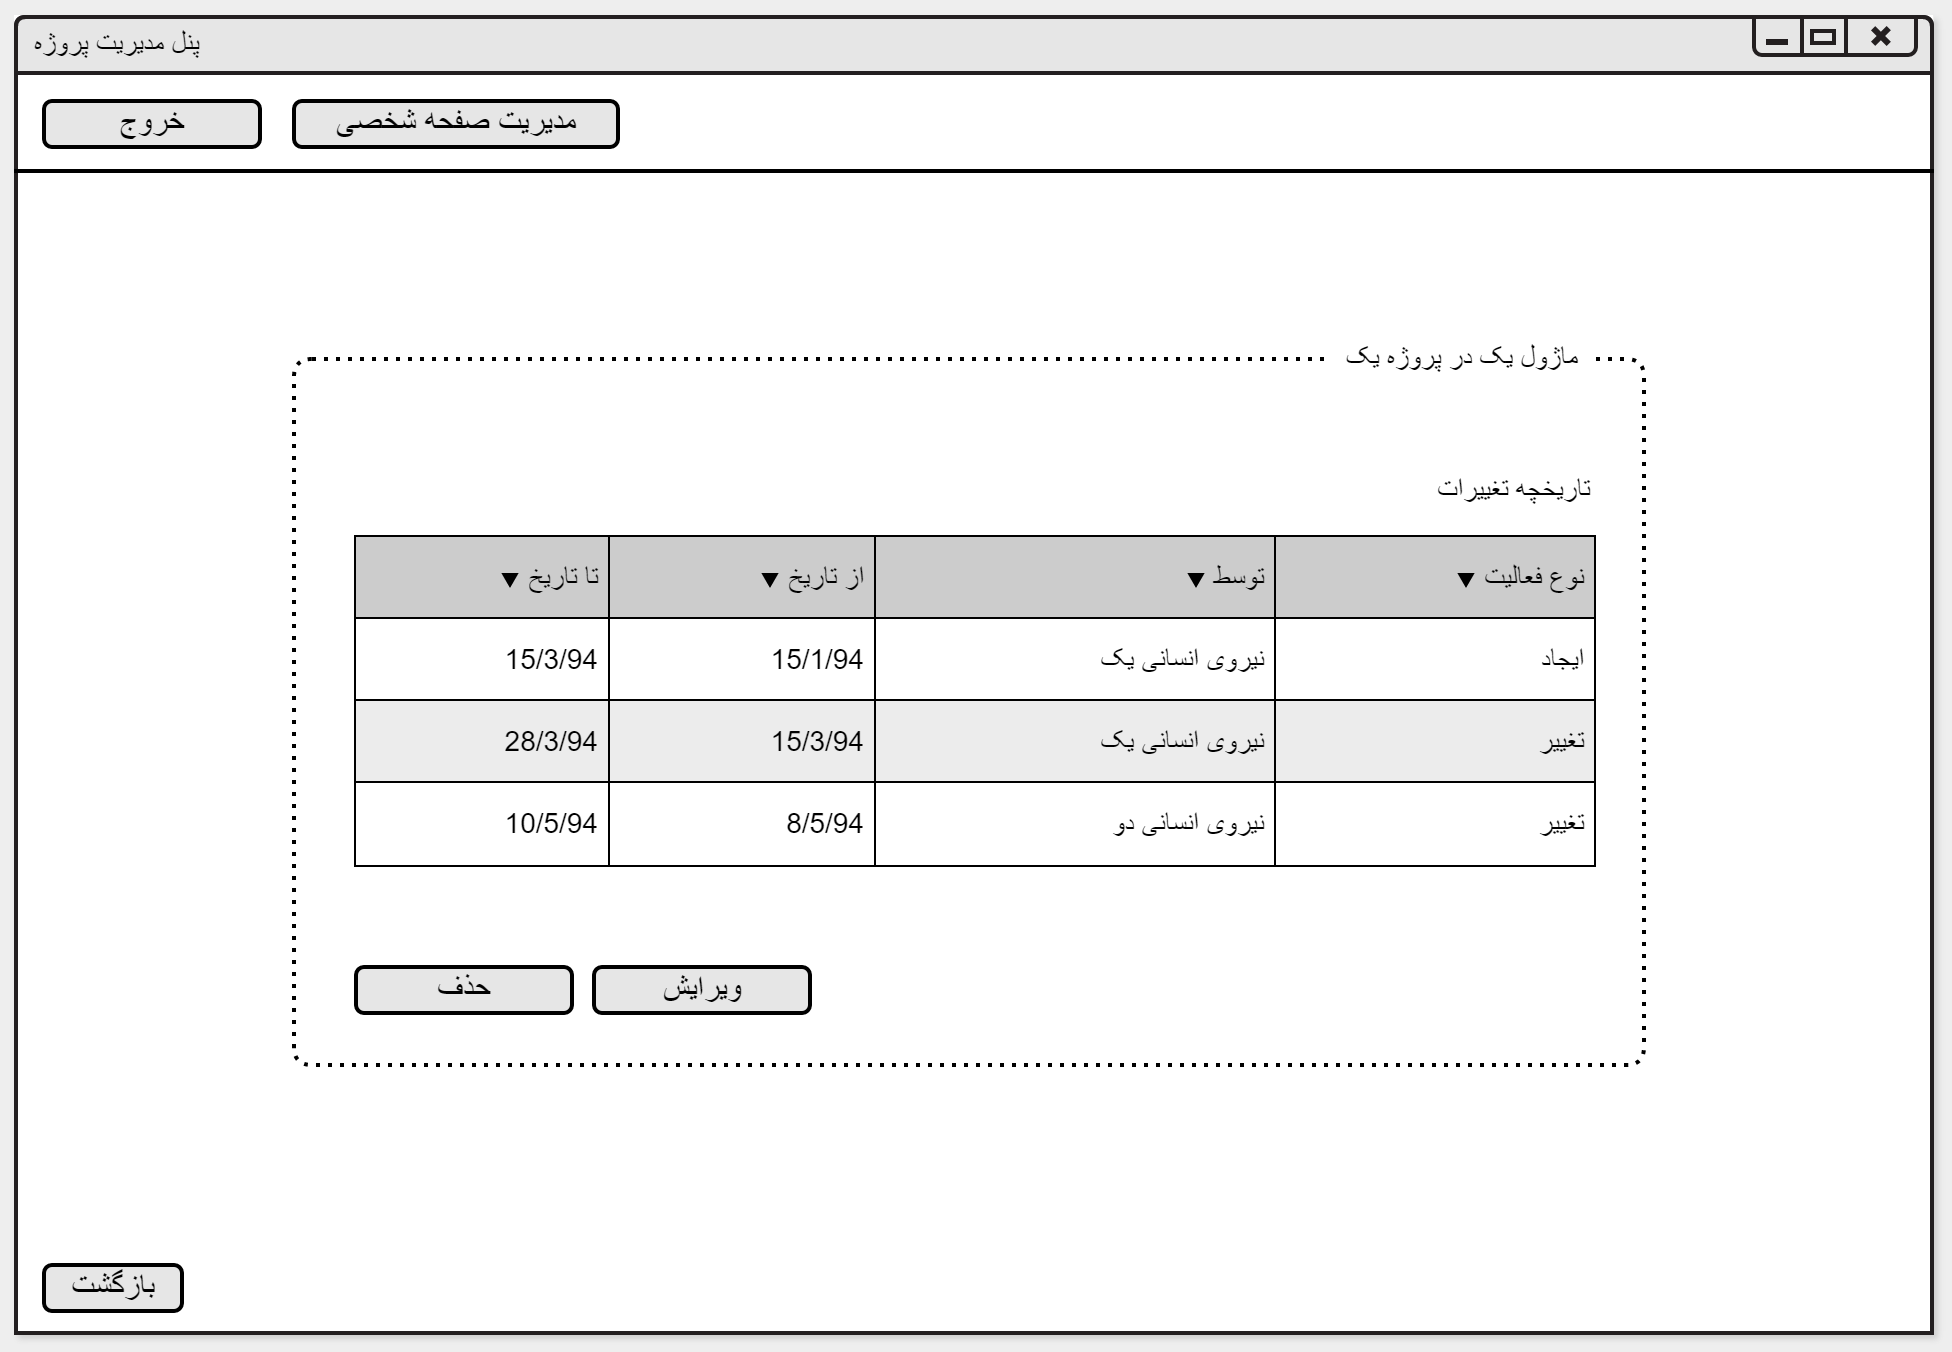
\includegraphics[width=\textwidth]{Prototype/ProjectManager/ModuleInformation.png}
\end{center}

\newpage
\vspace{1cm}
صفحه‌ی فهرست منابع مورد استفاده در پروژه 
\begin{center}
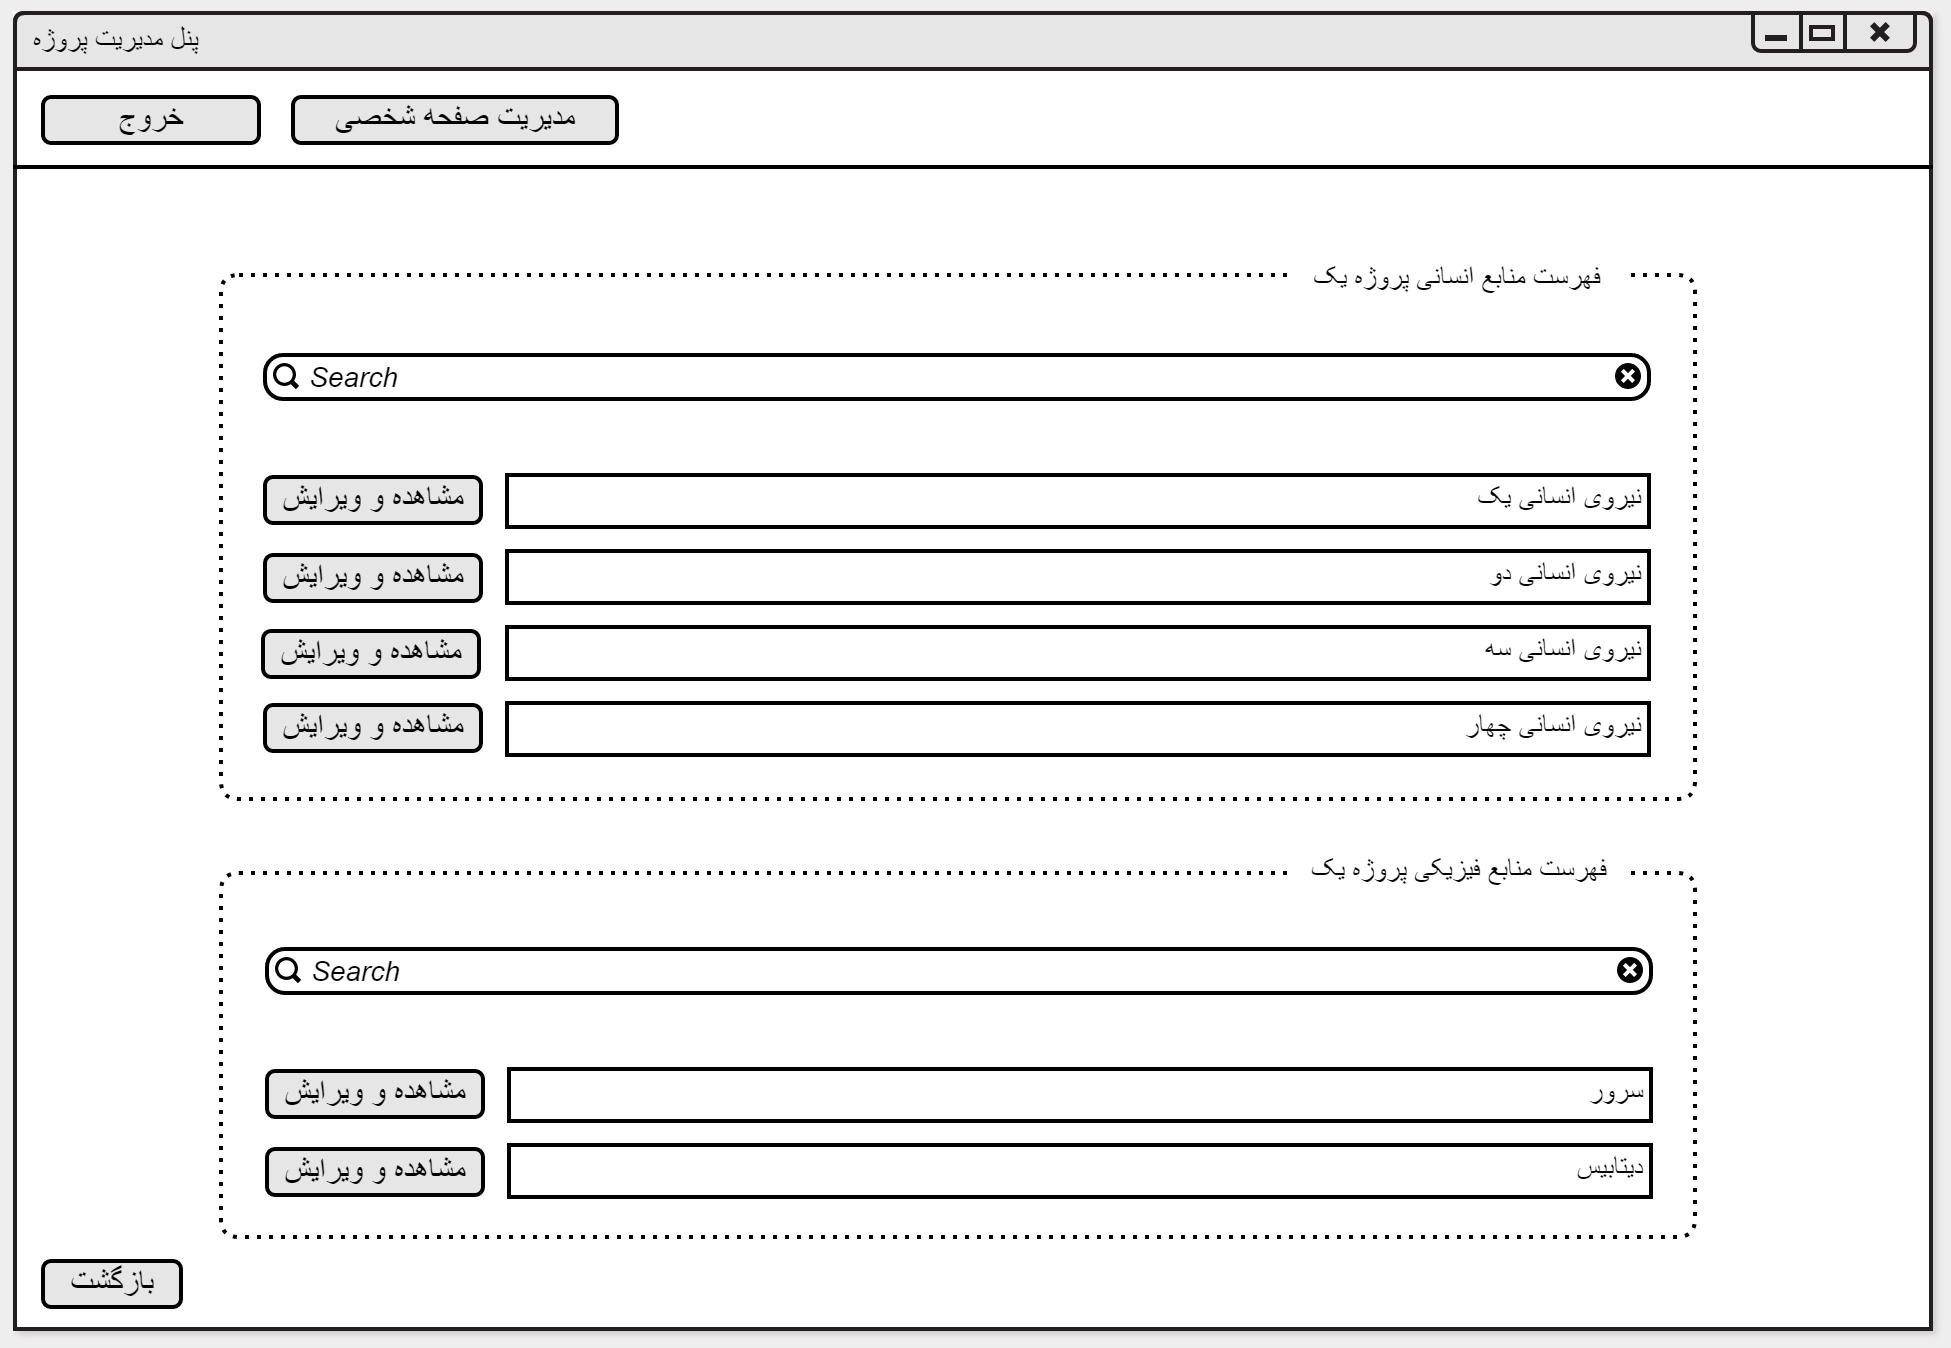
\includegraphics[width=\textwidth]{Prototype/ProjectManager/ProjectResourcesList.png}
\end{center}

\vspace{1cm}
صفحه‌ی اطلاعات منبع مورد استفاده در پروژه 
\begin{center}
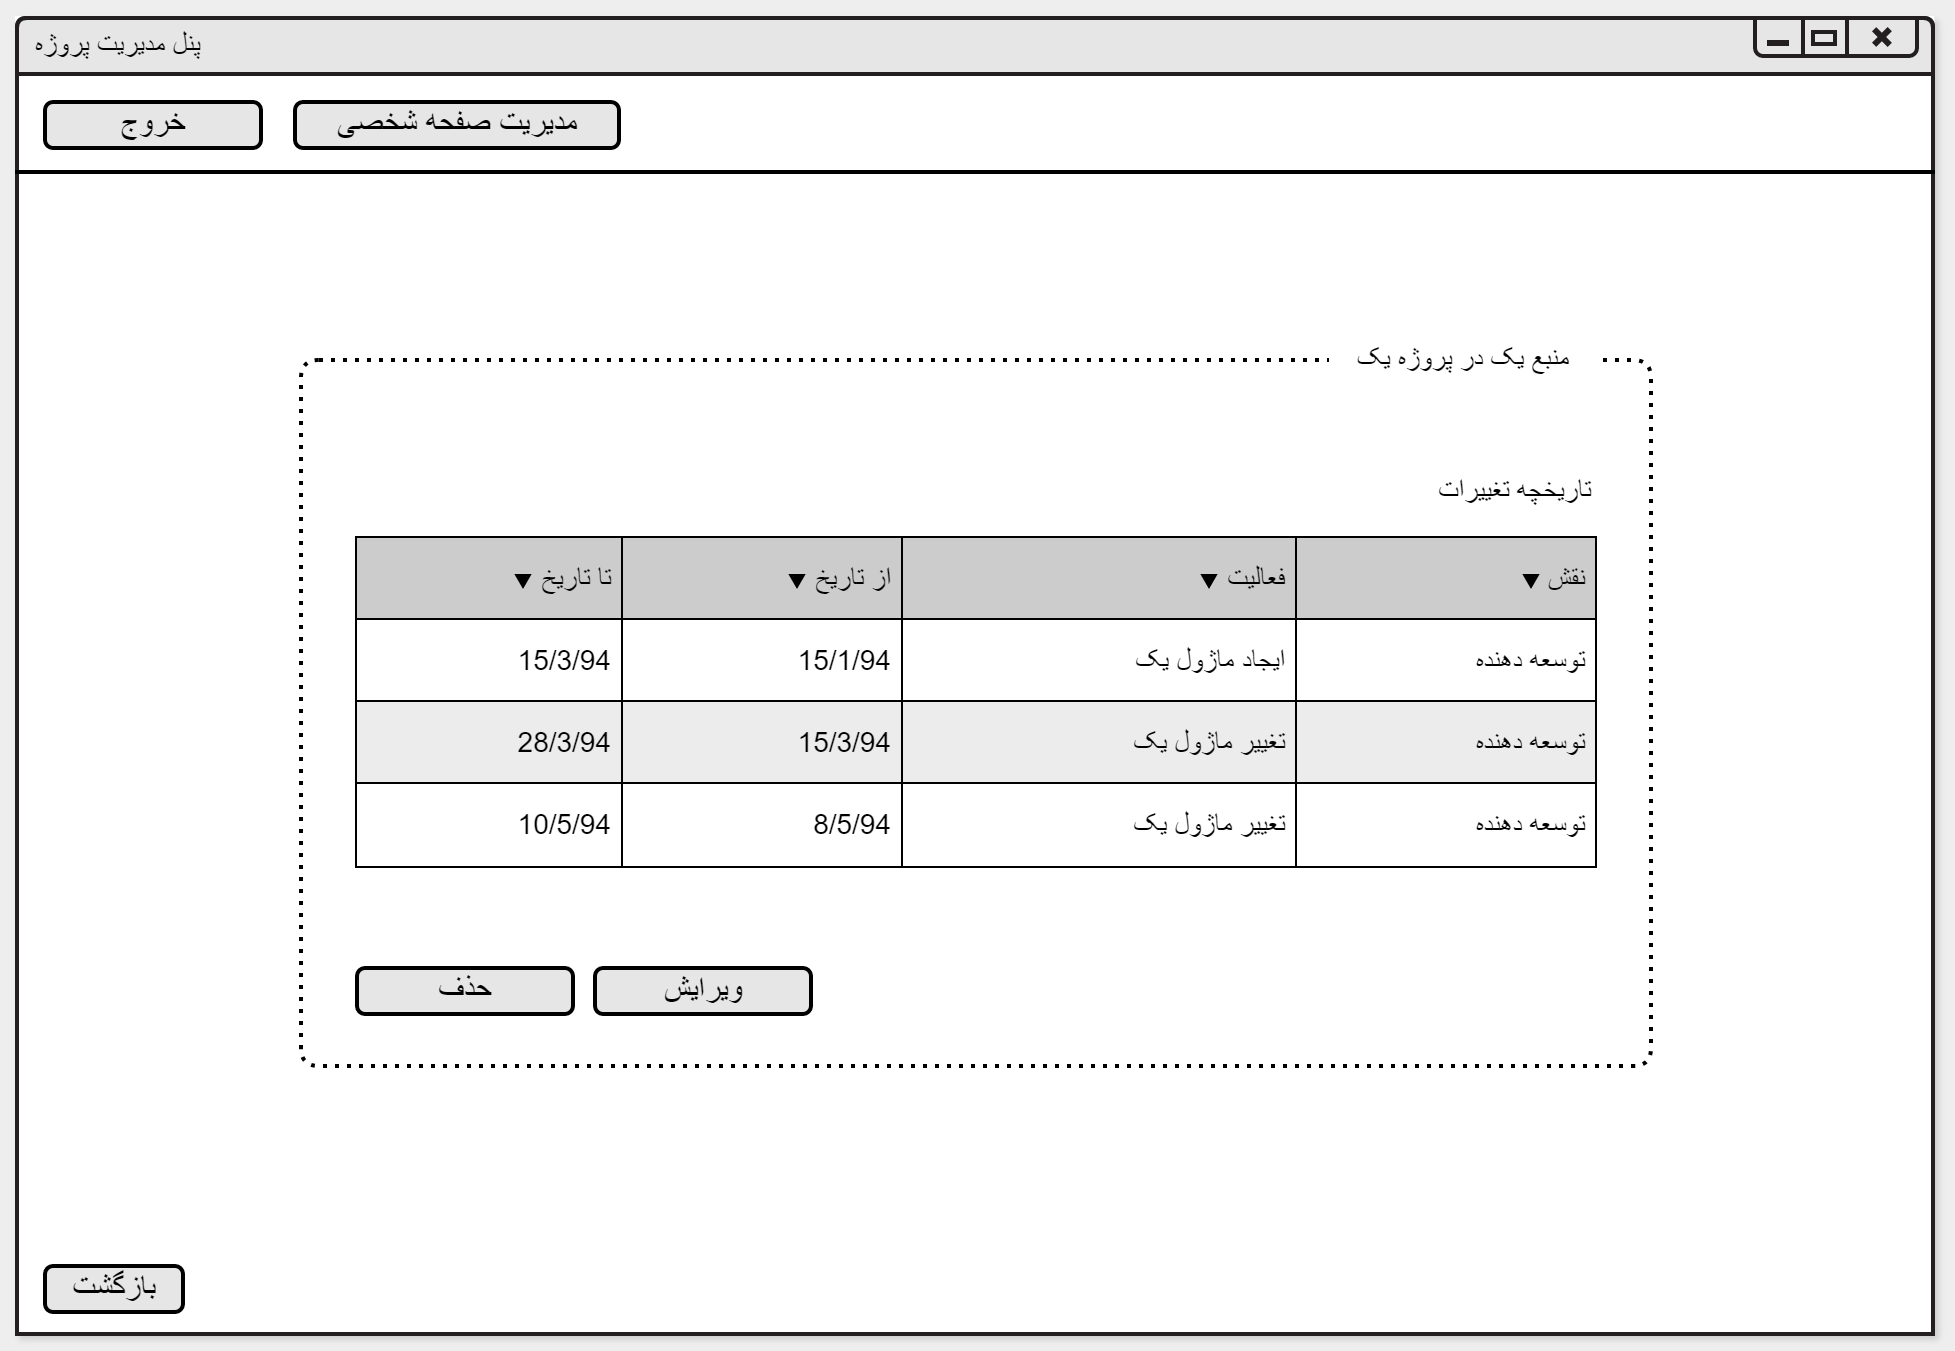
\includegraphics[width=\textwidth]{Prototype/ProjectManager/ResourceInformation.png}
\end{center}

\newpage
\vspace{1cm}
صفحه‌ی فهرست وظیفه‌ها بر اساس منبع
\begin{center}
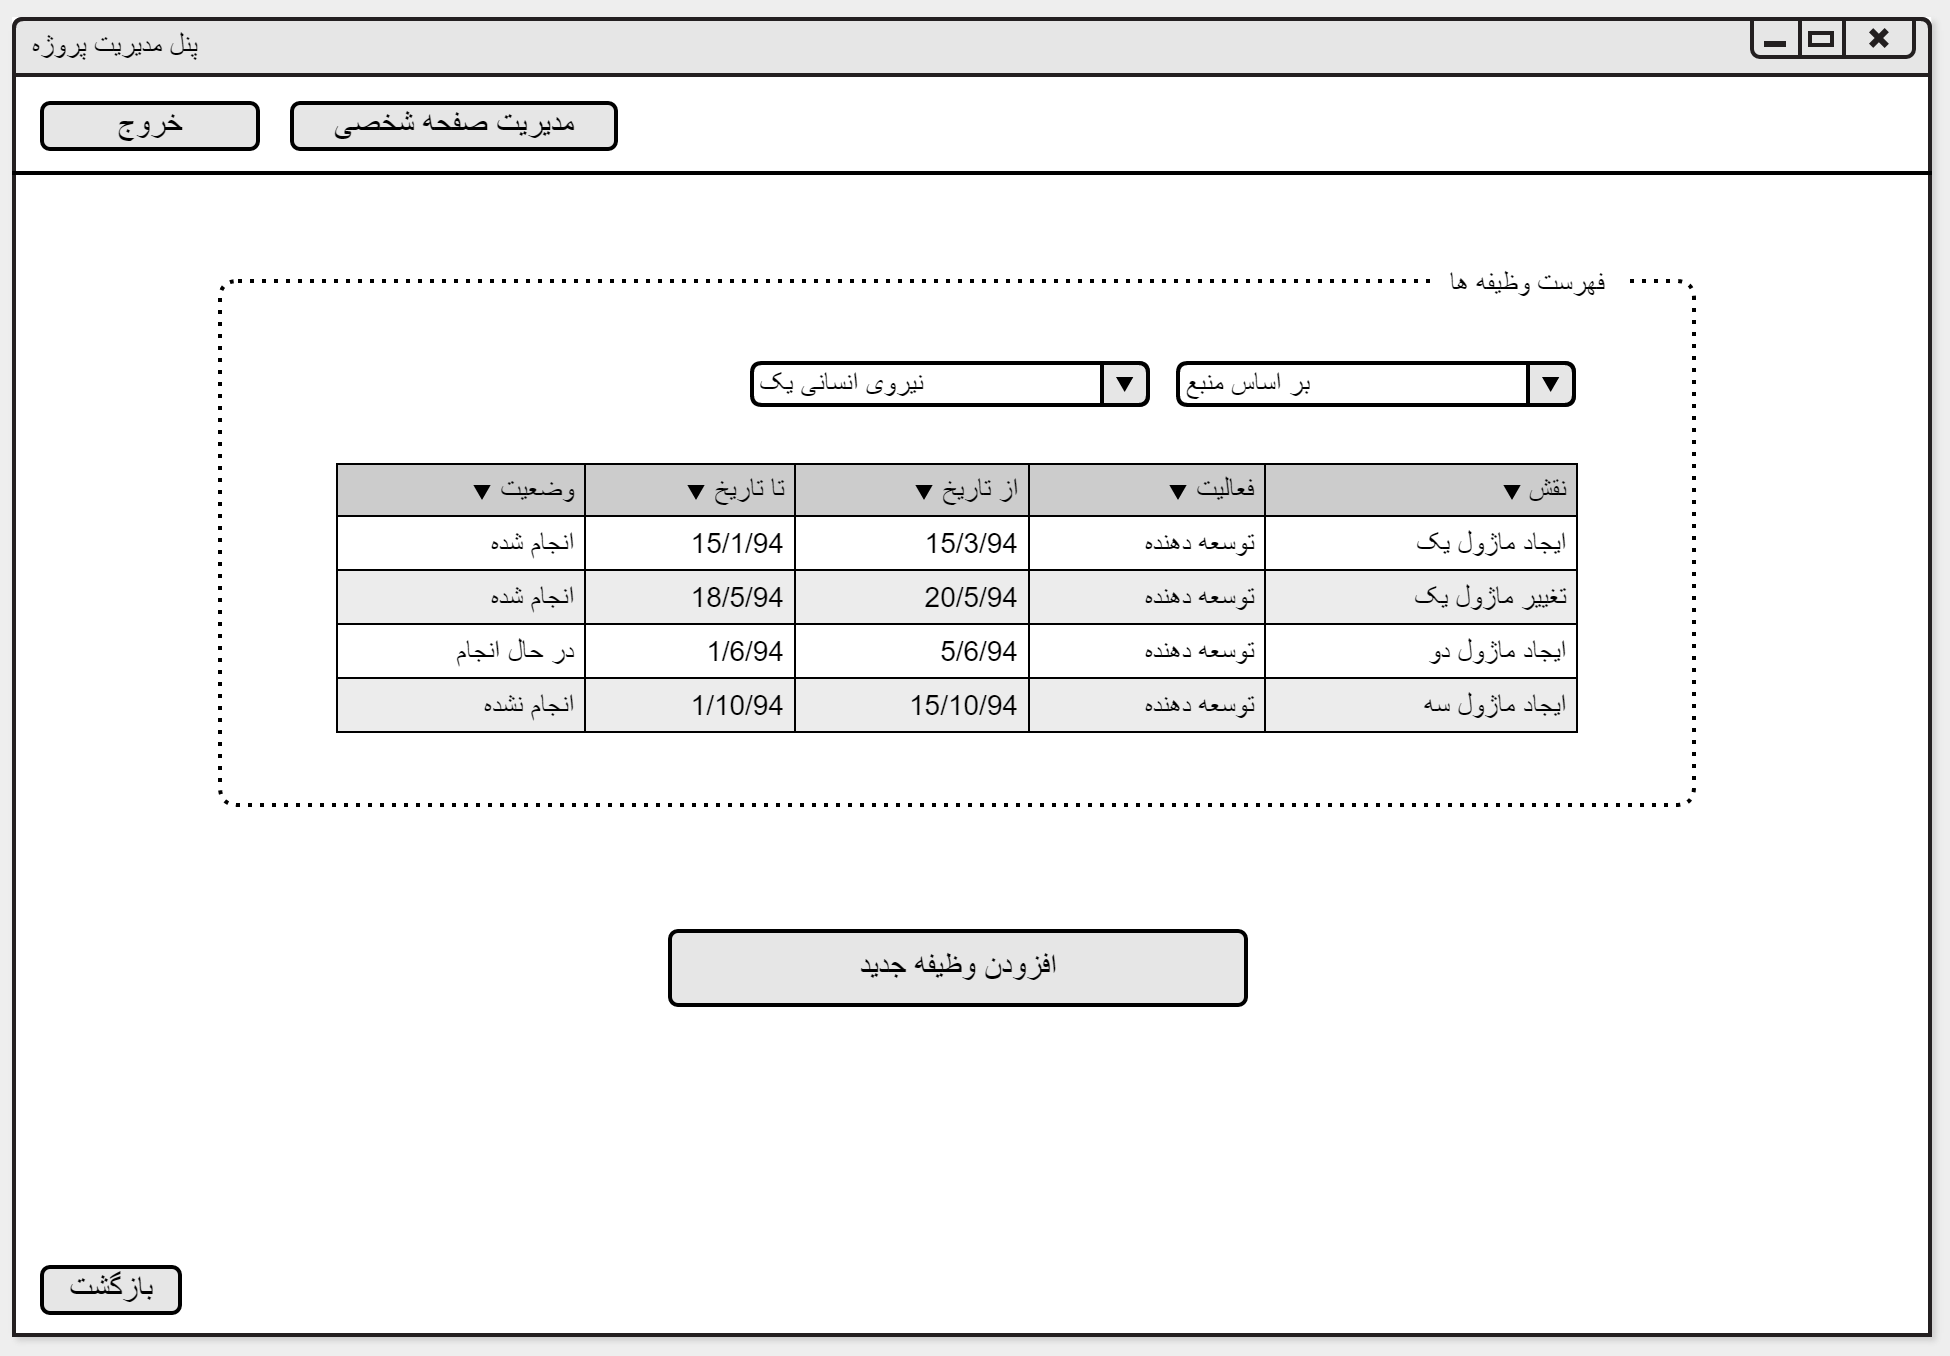
\includegraphics[width=\textwidth]{Prototype/ProjectManager/ProjectTasks1.png}
\end{center}

\vspace{1cm}
صفحه‌ی فهرست وظیفه‌ها بر اساس زمان
\begin{center}
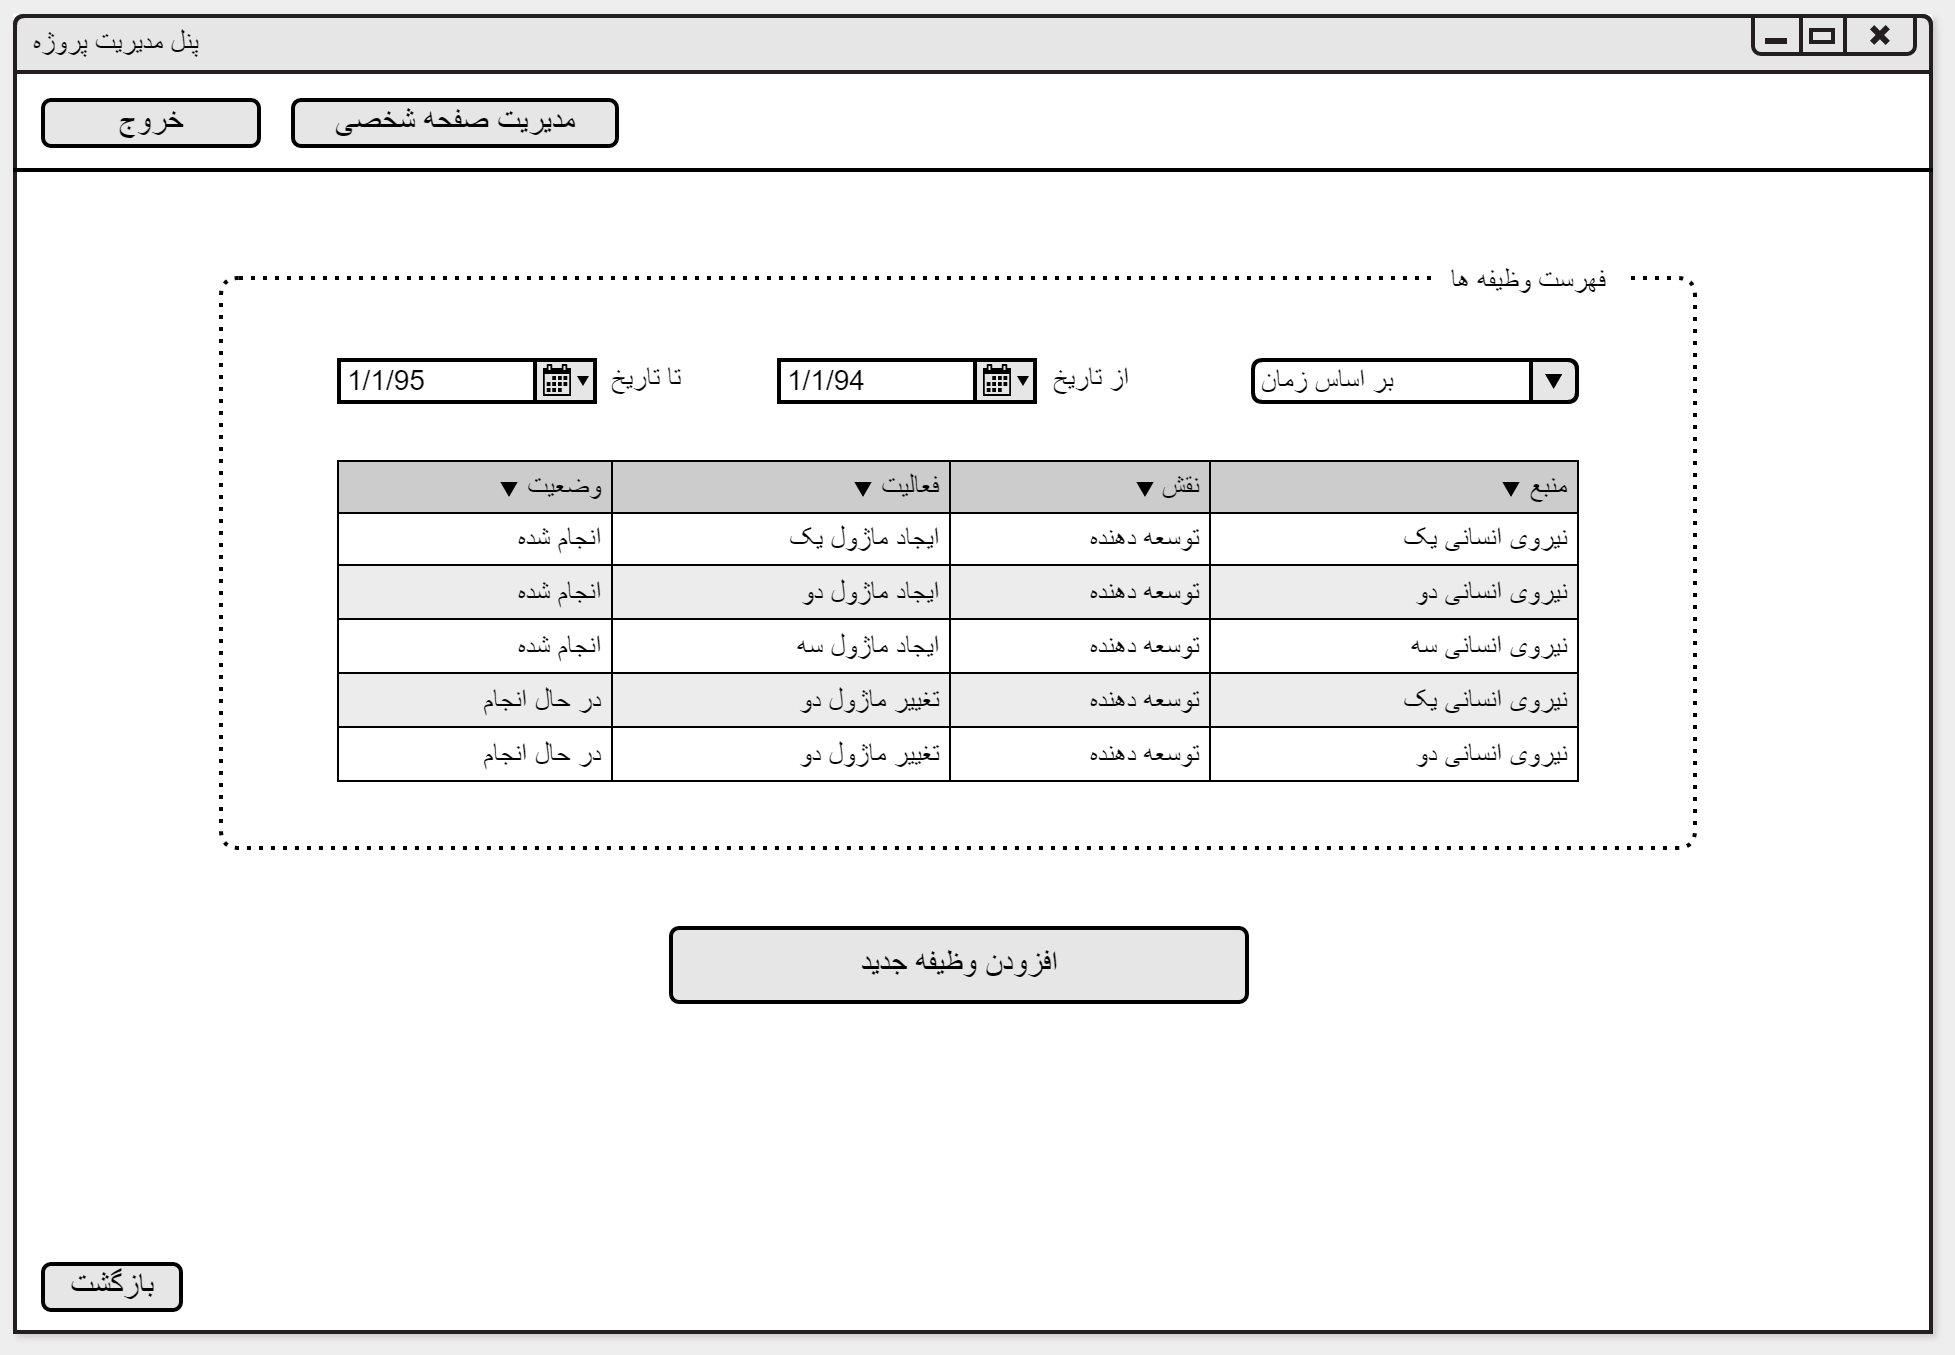
\includegraphics[width=\textwidth]{Prototype/ProjectManager/ProjectTasks2.png}
\end{center}

\newpage
\vspace{1cm}
صفحه‌ی فهرست نیازمندی‌های پروژه 
\begin{center}
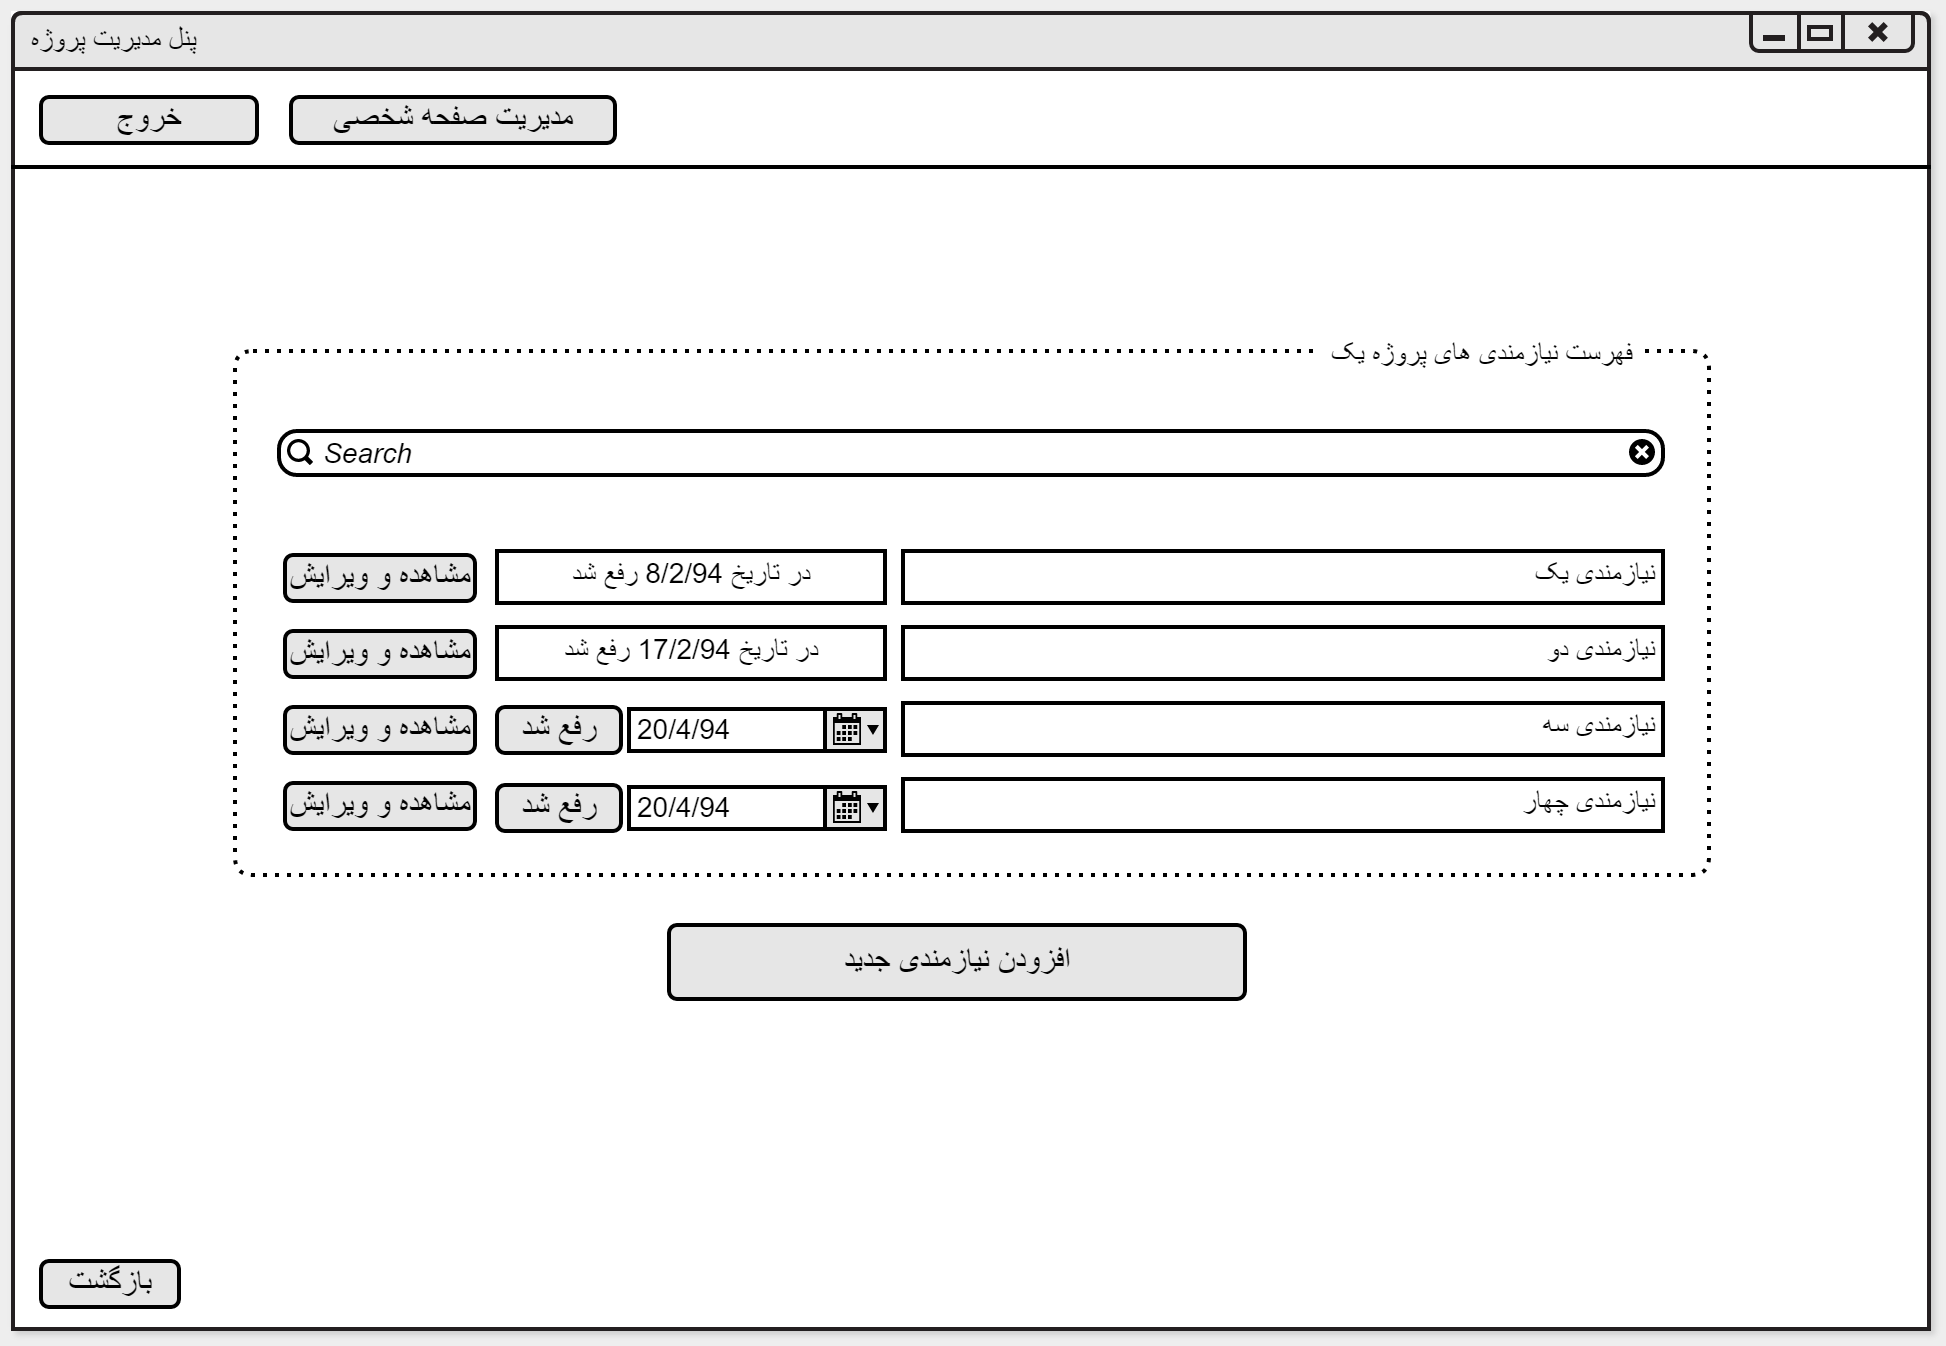
\includegraphics[width=\textwidth]{Prototype/ProjectManager/ProjectRequirements.png}
\end{center}

\newpage
\subsection{صفحات مدیریت کل}

\vspace{1cm}
صفحه‌ی پنل اصلی مدیر کل
\begin{center}
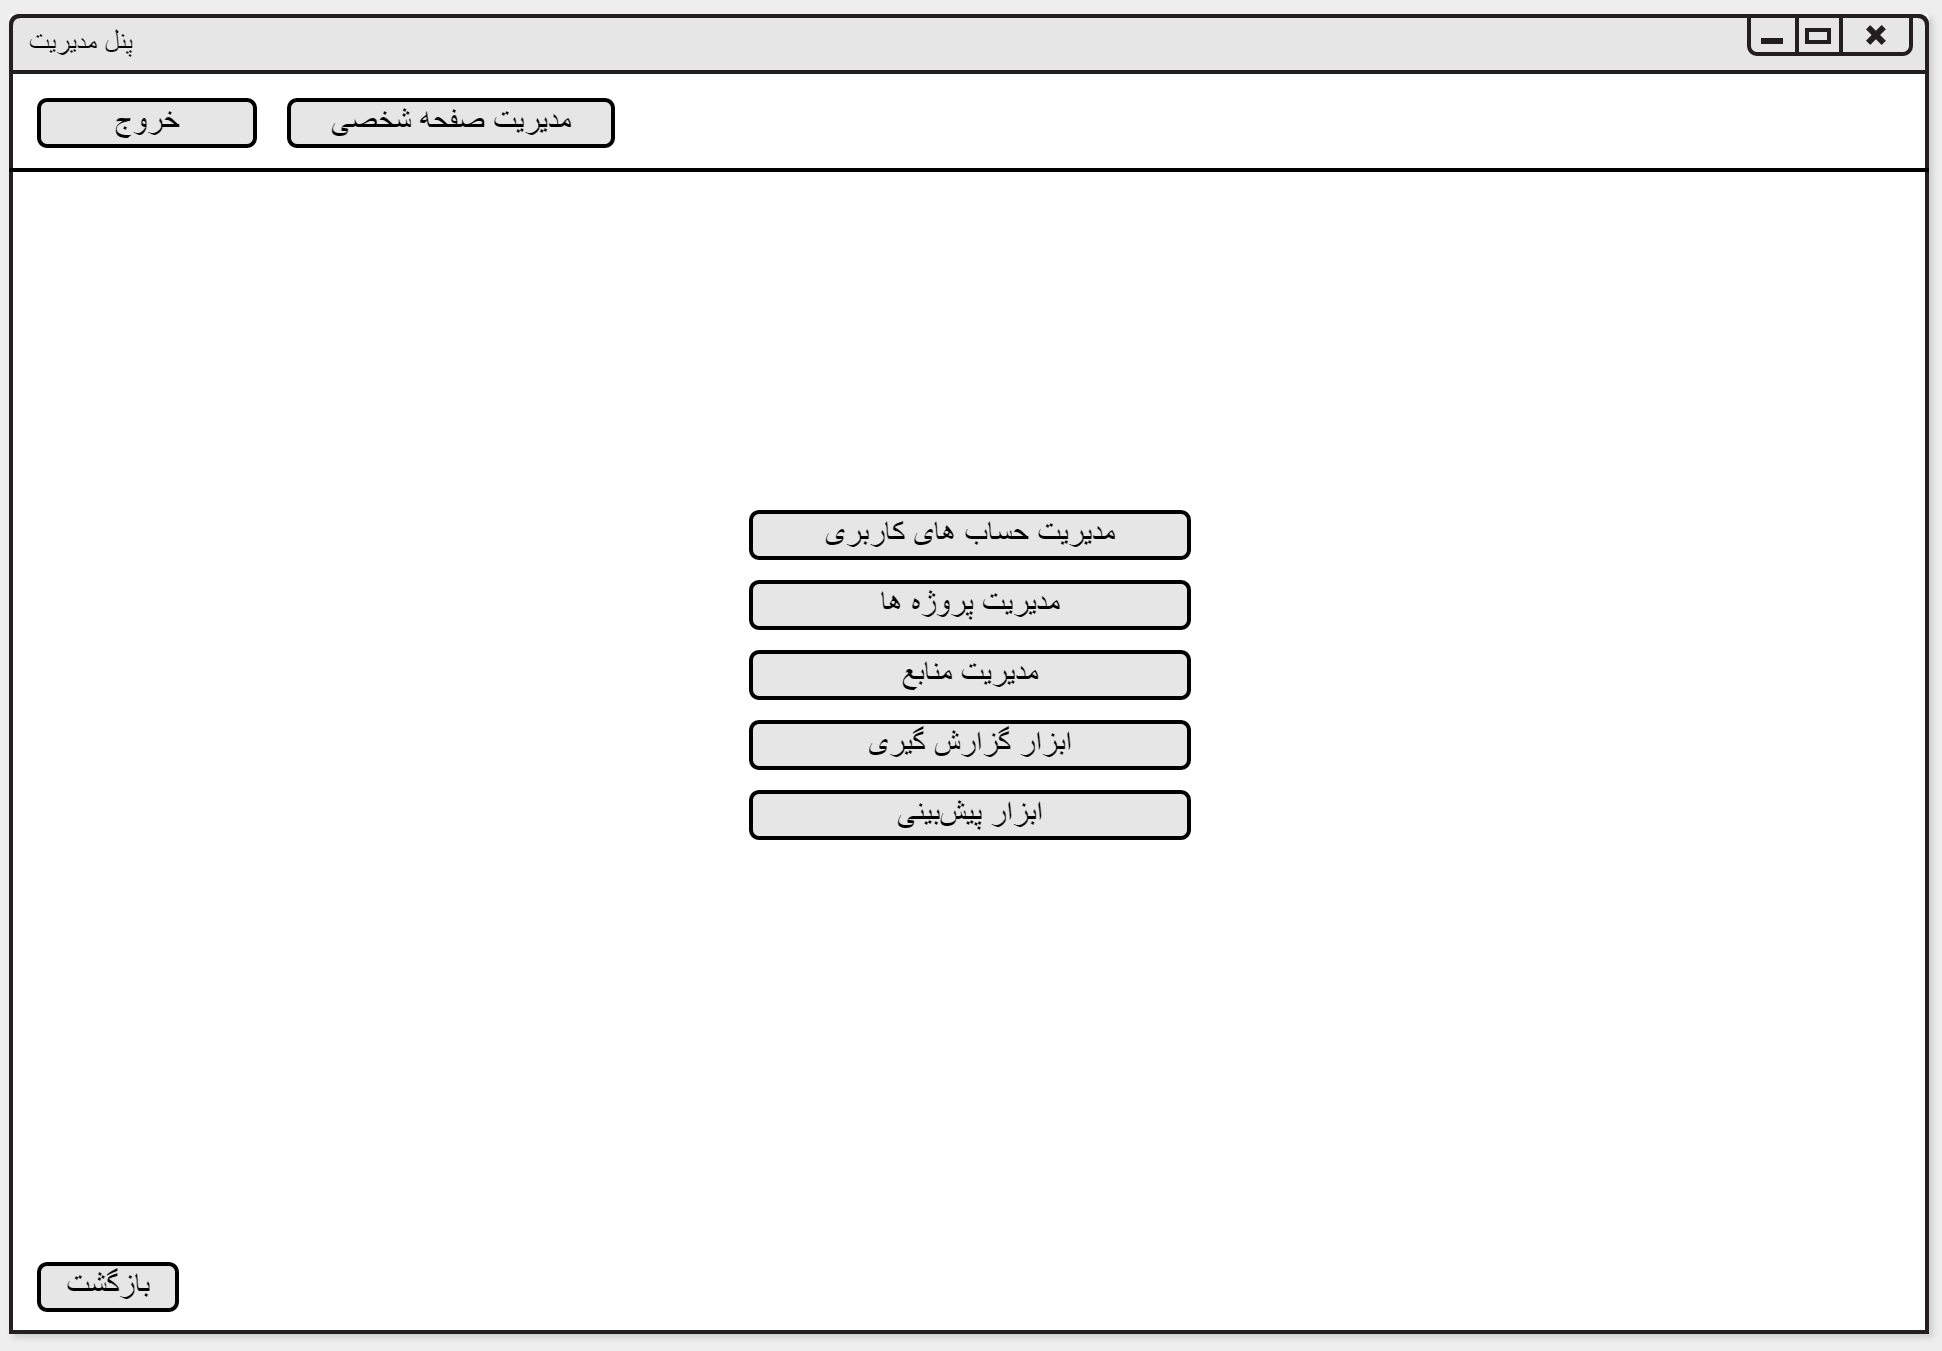
\includegraphics[width=\textwidth]{Prototype/HeadManager/HeadManagerMainPanel.png}
\end{center}

\newpage
\vspace{1cm}
صفحه‌ی مدیریت حساب‌های کاربری 
\begin{center}
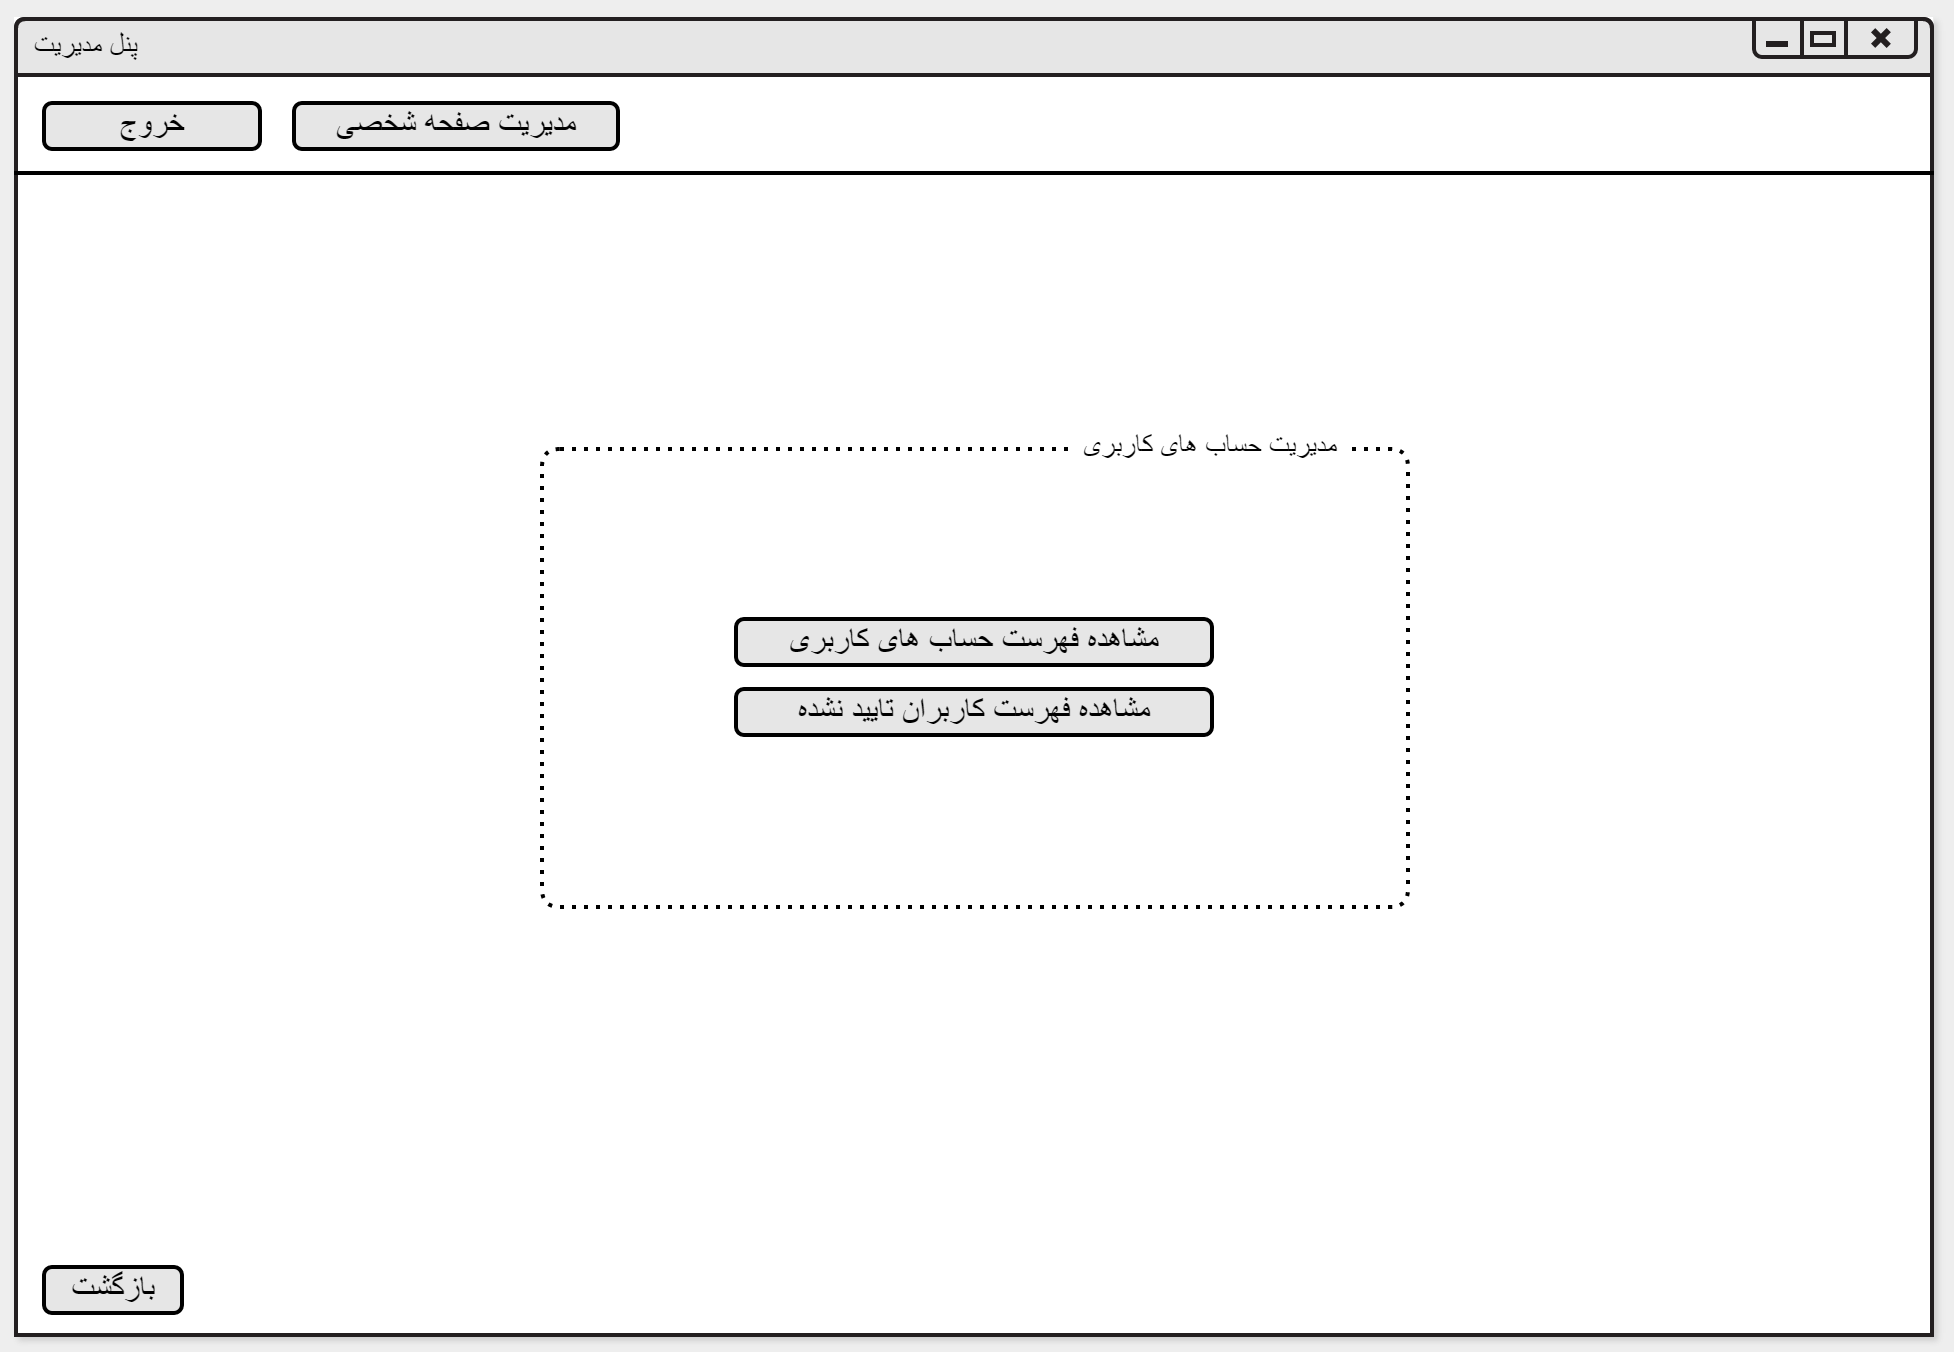
\includegraphics[width=\textwidth]{Prototype/HeadManager/AccountManager.png}
\end{center}

\newpage
\vspace{1cm}
صفحه‌ی فهرست حساب‌های کاربری تایید شده
\begin{center}
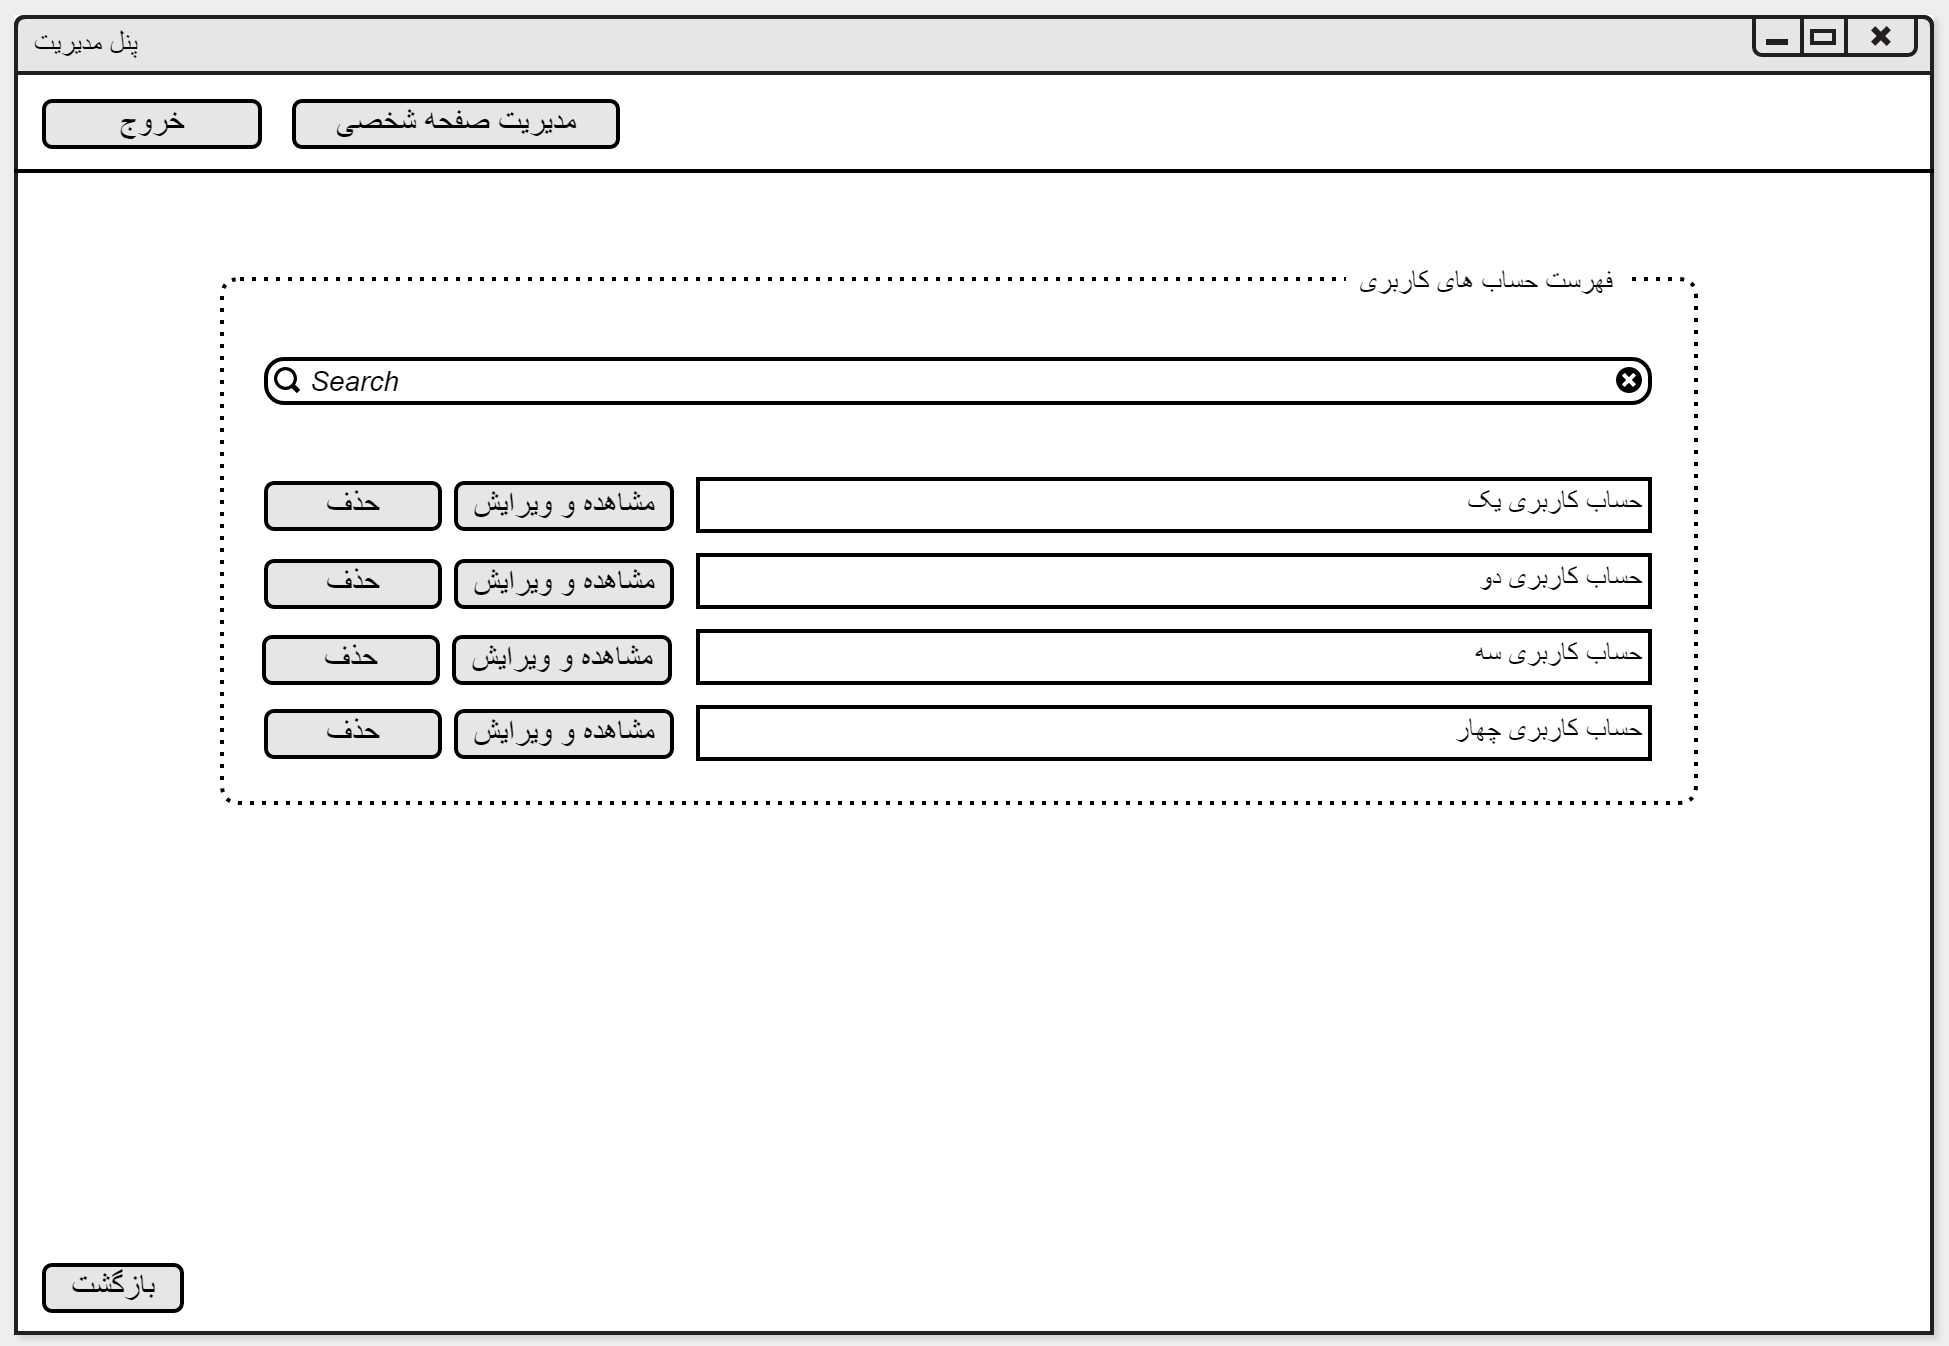
\includegraphics[width=\textwidth]{Prototype/HeadManager/VerifiedAccountsList.png}
\end{center}

\vspace{1cm}
صفحه‌ی فهرست حساب‌های کاربری تایید نشده
\begin{center}
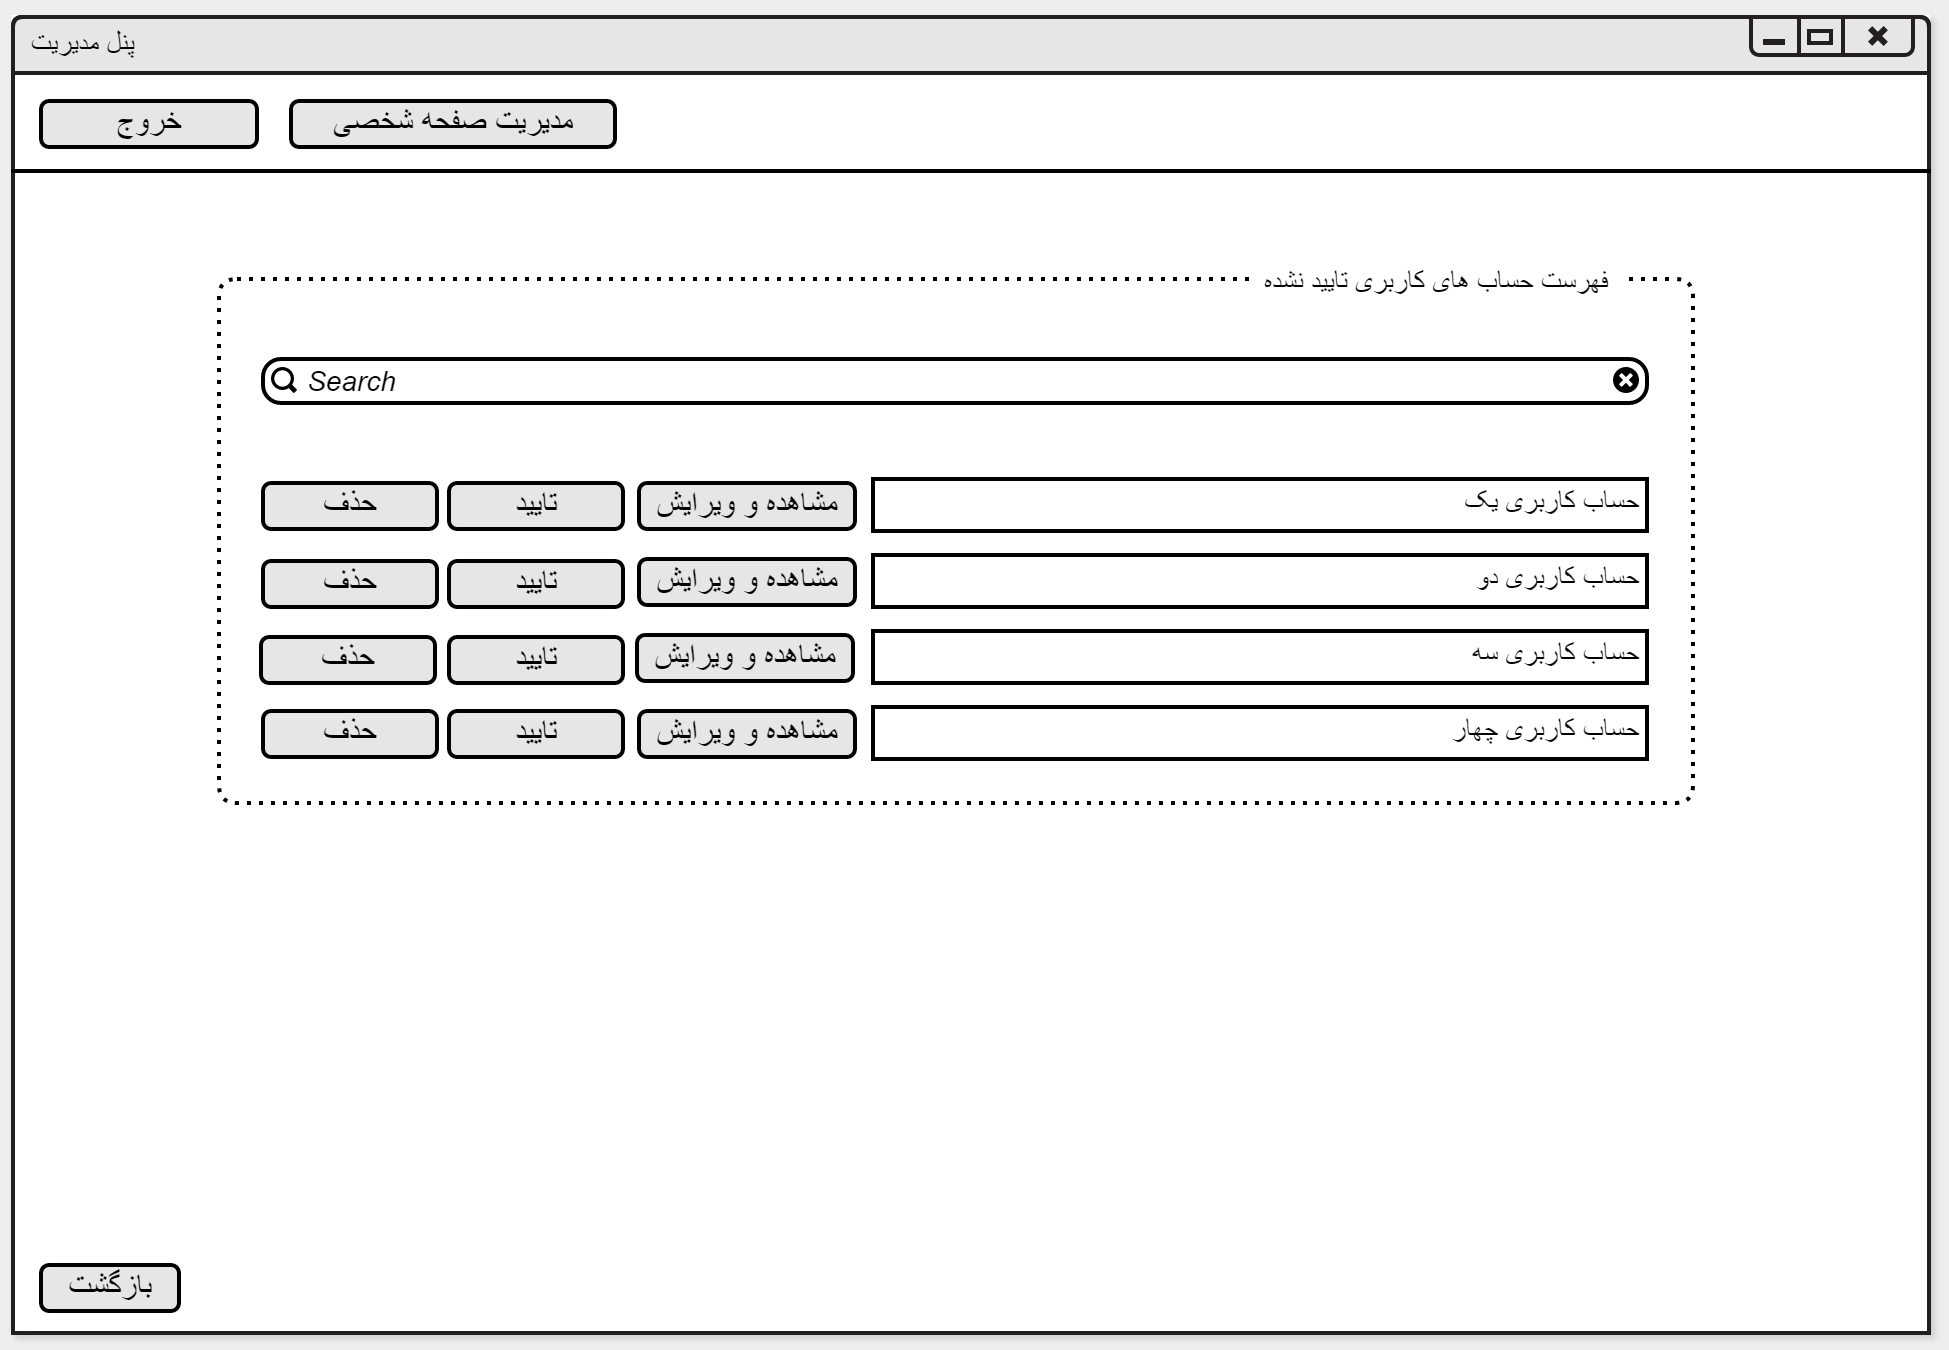
\includegraphics[width=\textwidth]{Prototype/HeadManager/UnverifiedAccountsList.png}
\end{center}

\newpage
\vspace{1cm}
صفحه‌ی اطلاعات یک حساب کاربری و تغییر سمت 
\begin{center}
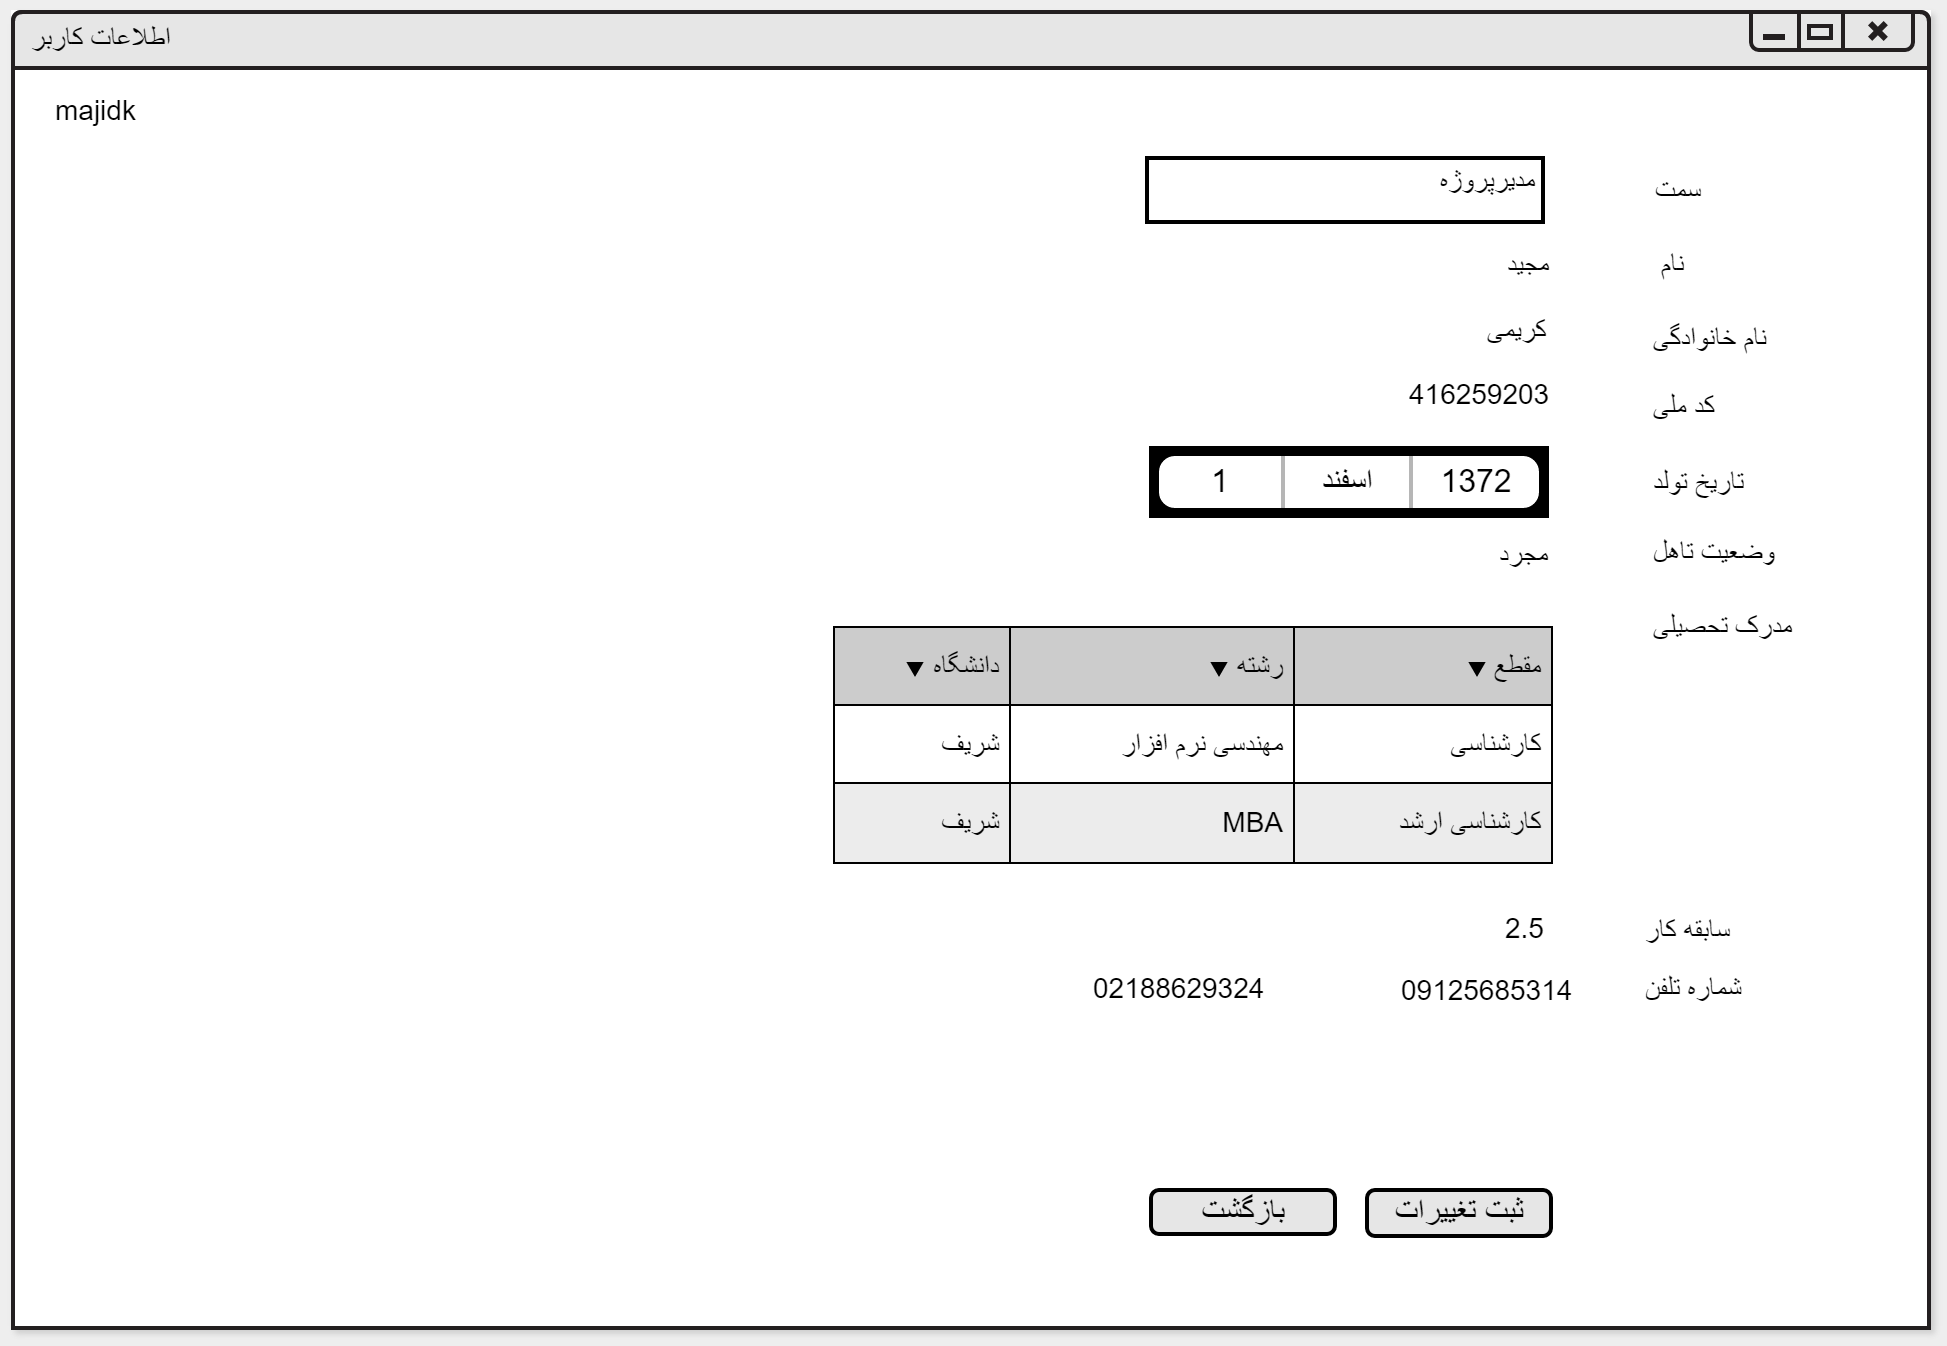
\includegraphics[width=\textwidth]{Prototype/HeadManager/ChangePosition.png}
\end{center}

\newpage
\vspace{1cm}
صفحه‌ی مدیریت پروژه‌ها
\begin{center}
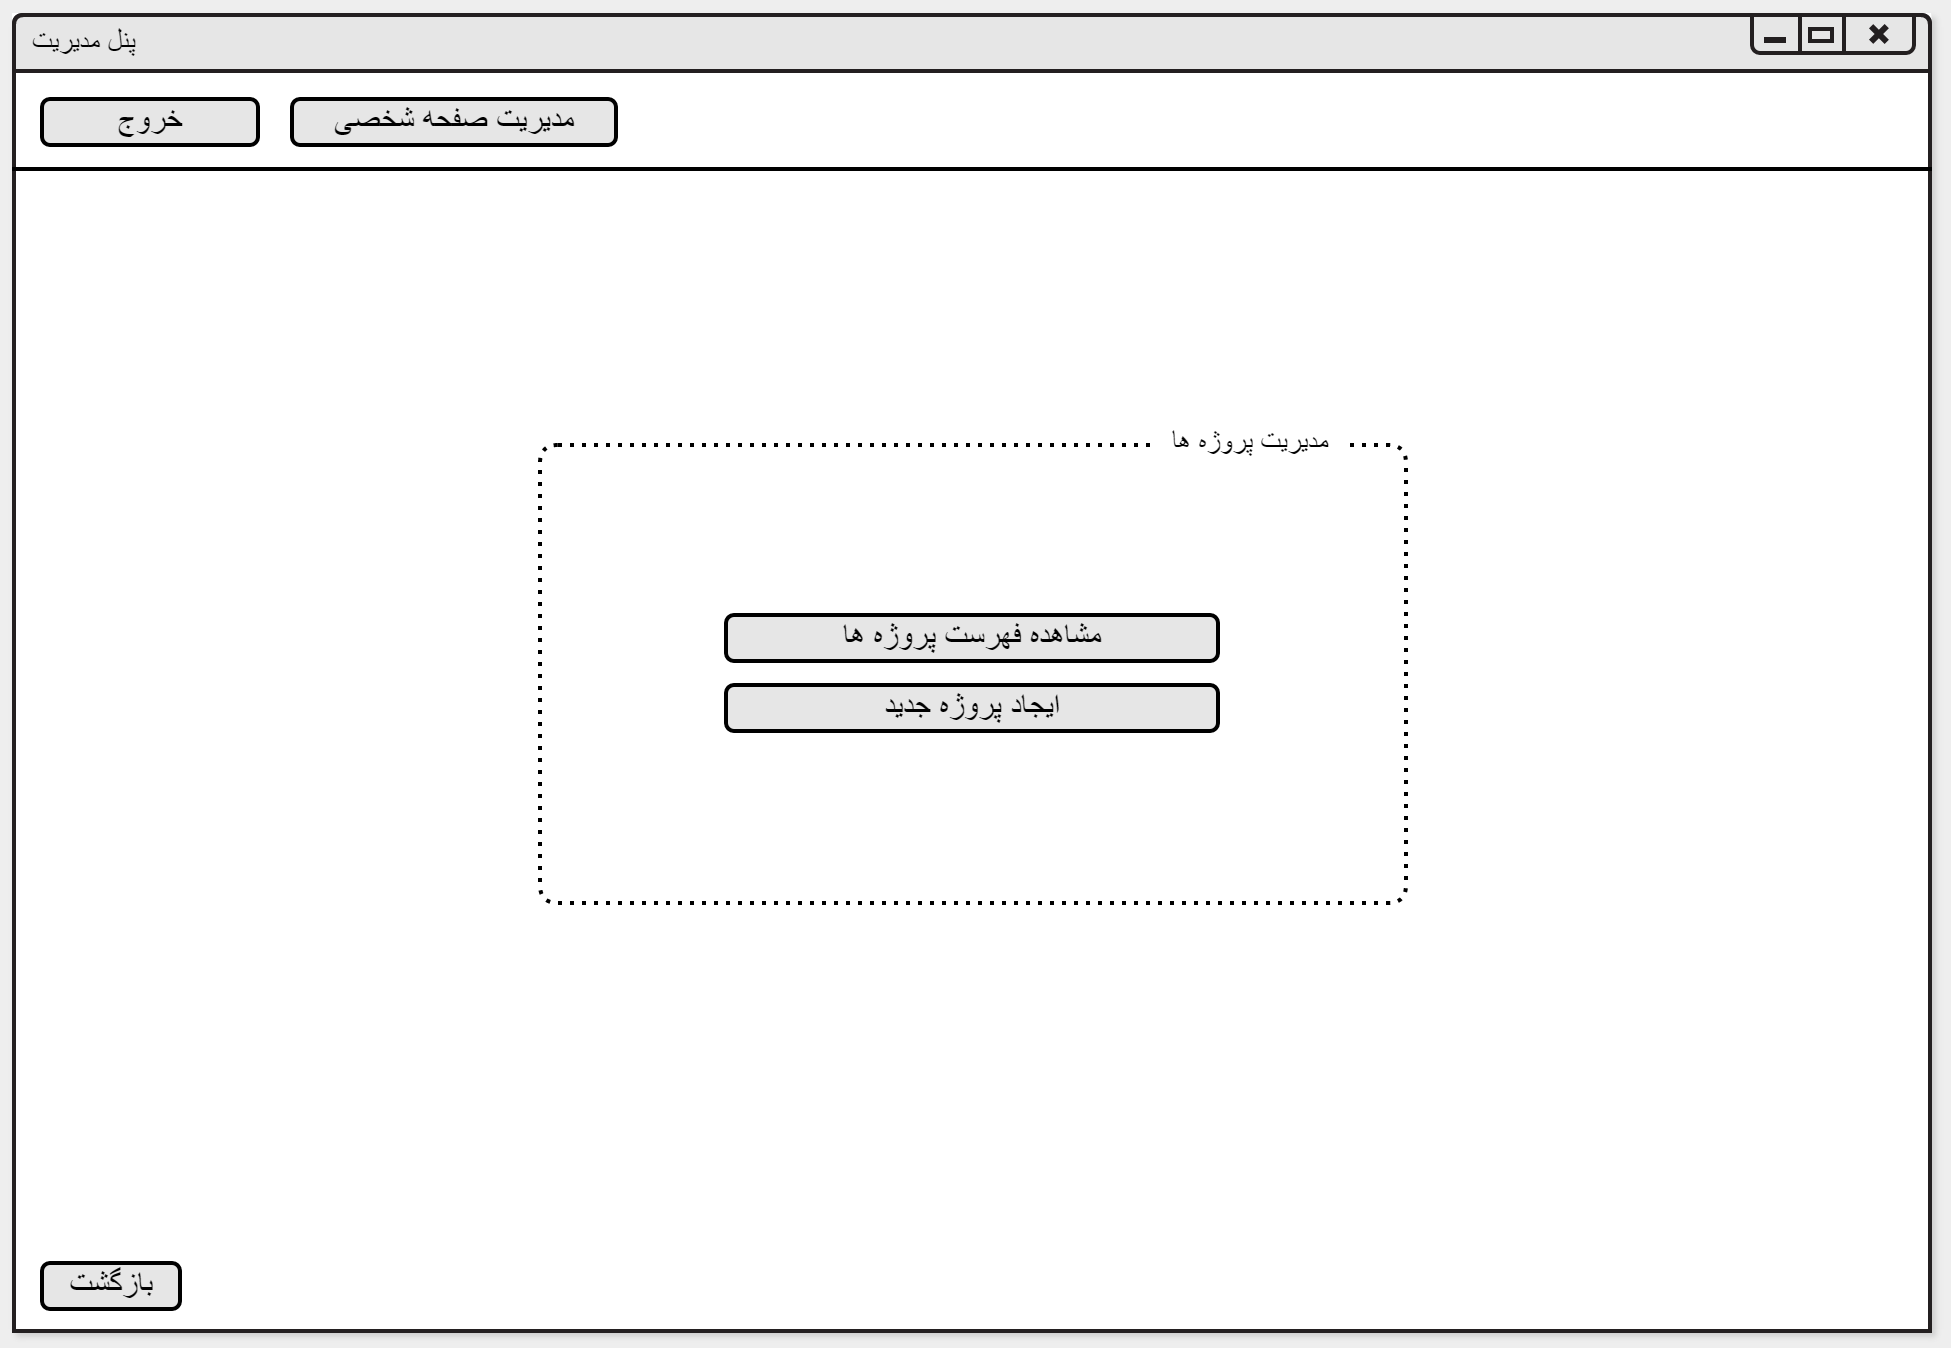
\includegraphics[width=\textwidth]{Prototype/HeadManager/ProjectsManagement.png}
\end{center}

\vspace{1cm}
صفحه‌ی فهرست پروژه‌ها
\begin{center}
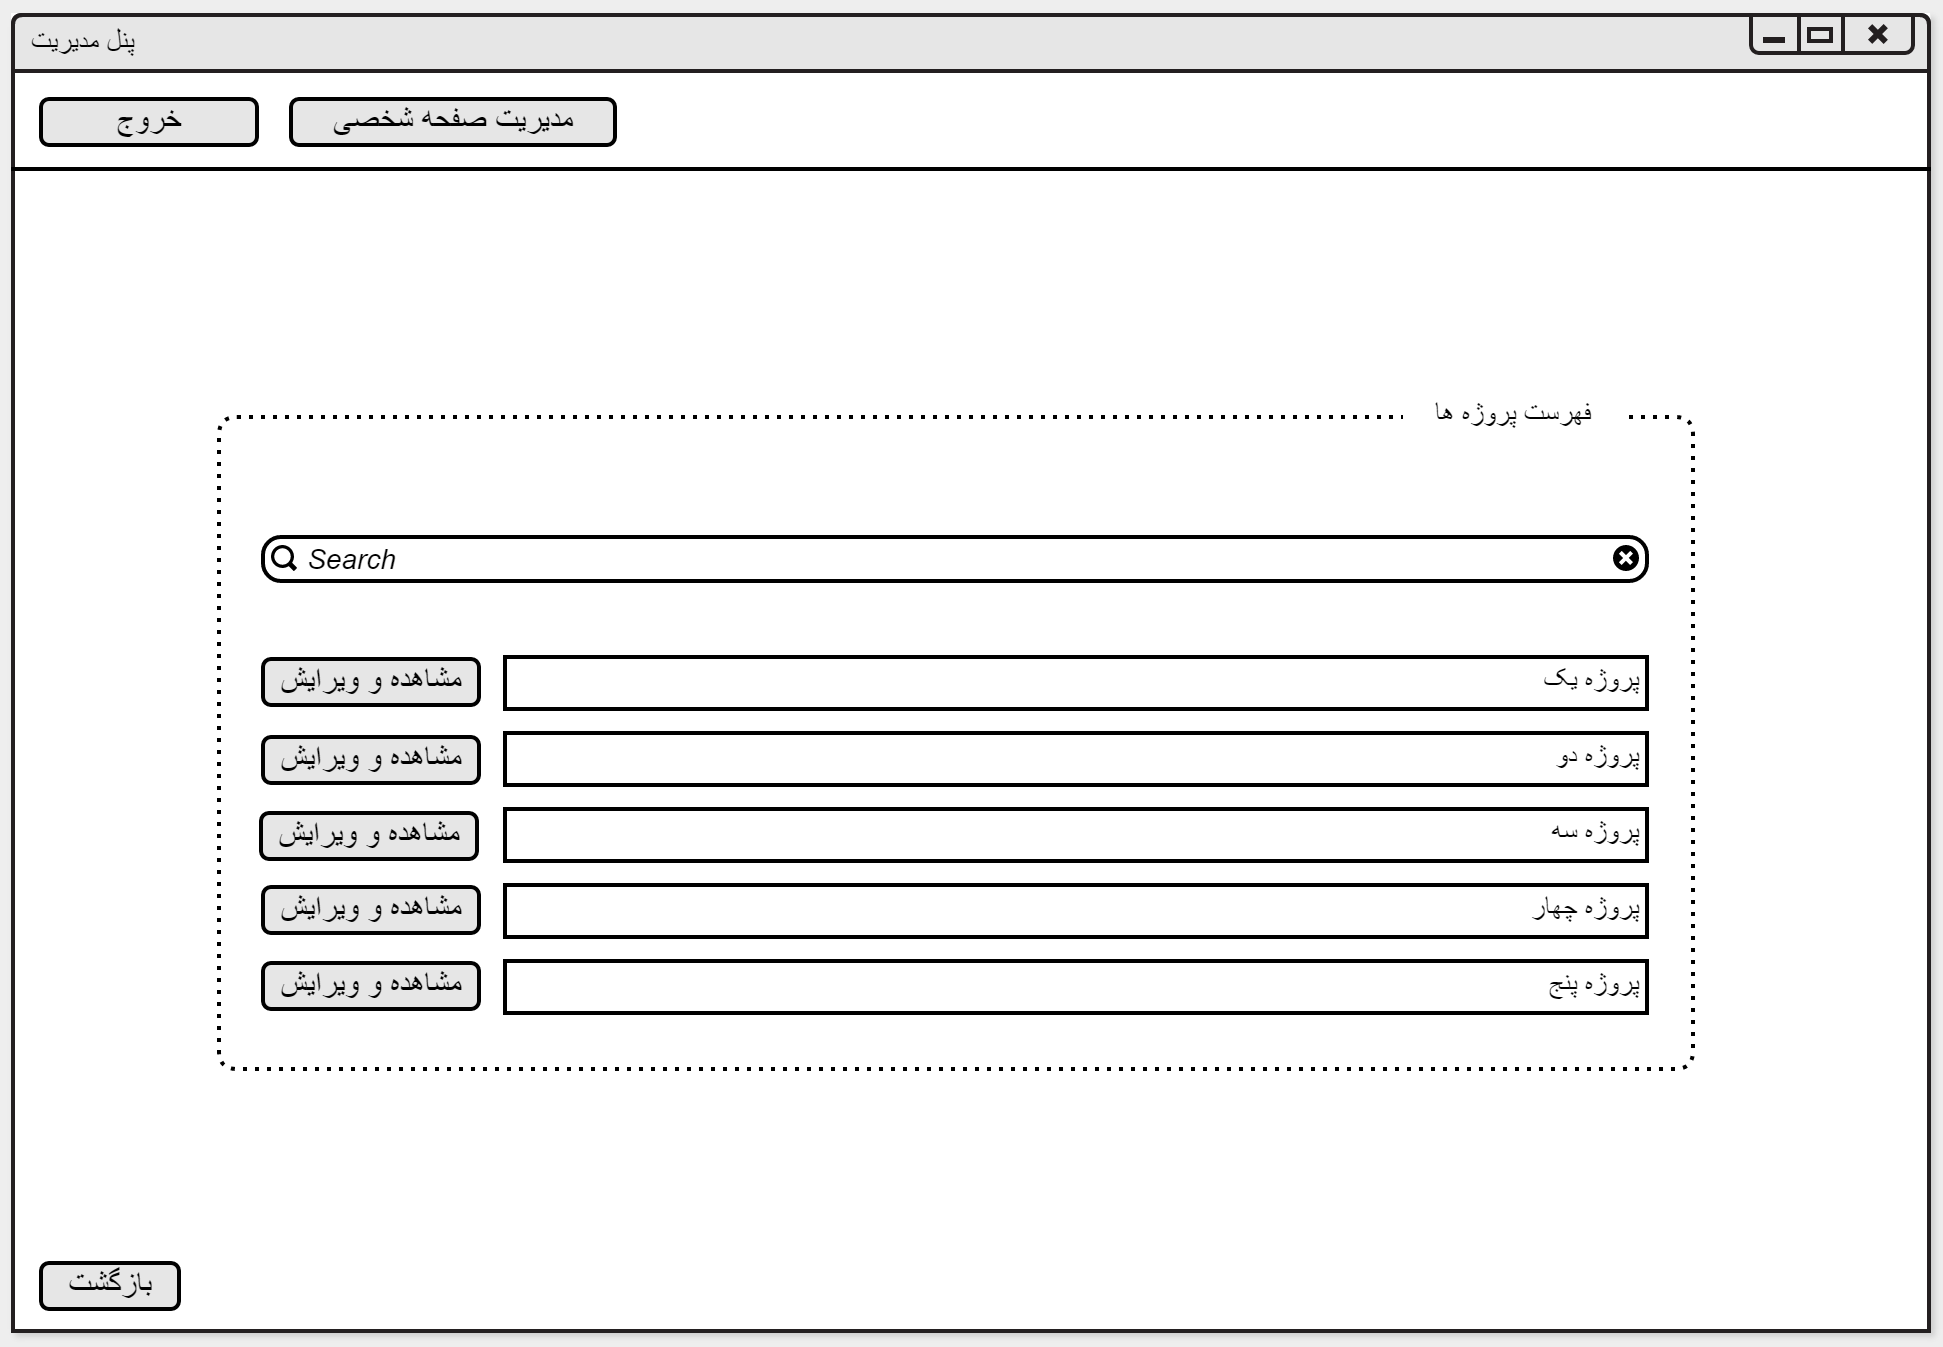
\includegraphics[width=\textwidth]{Prototype/HeadManager/HeadManagerProjectsList.png}
\end{center}

\newpage
\vspace{1cm}
صفحه‌ی تخصیص منابع به پروژه
\begin{center}
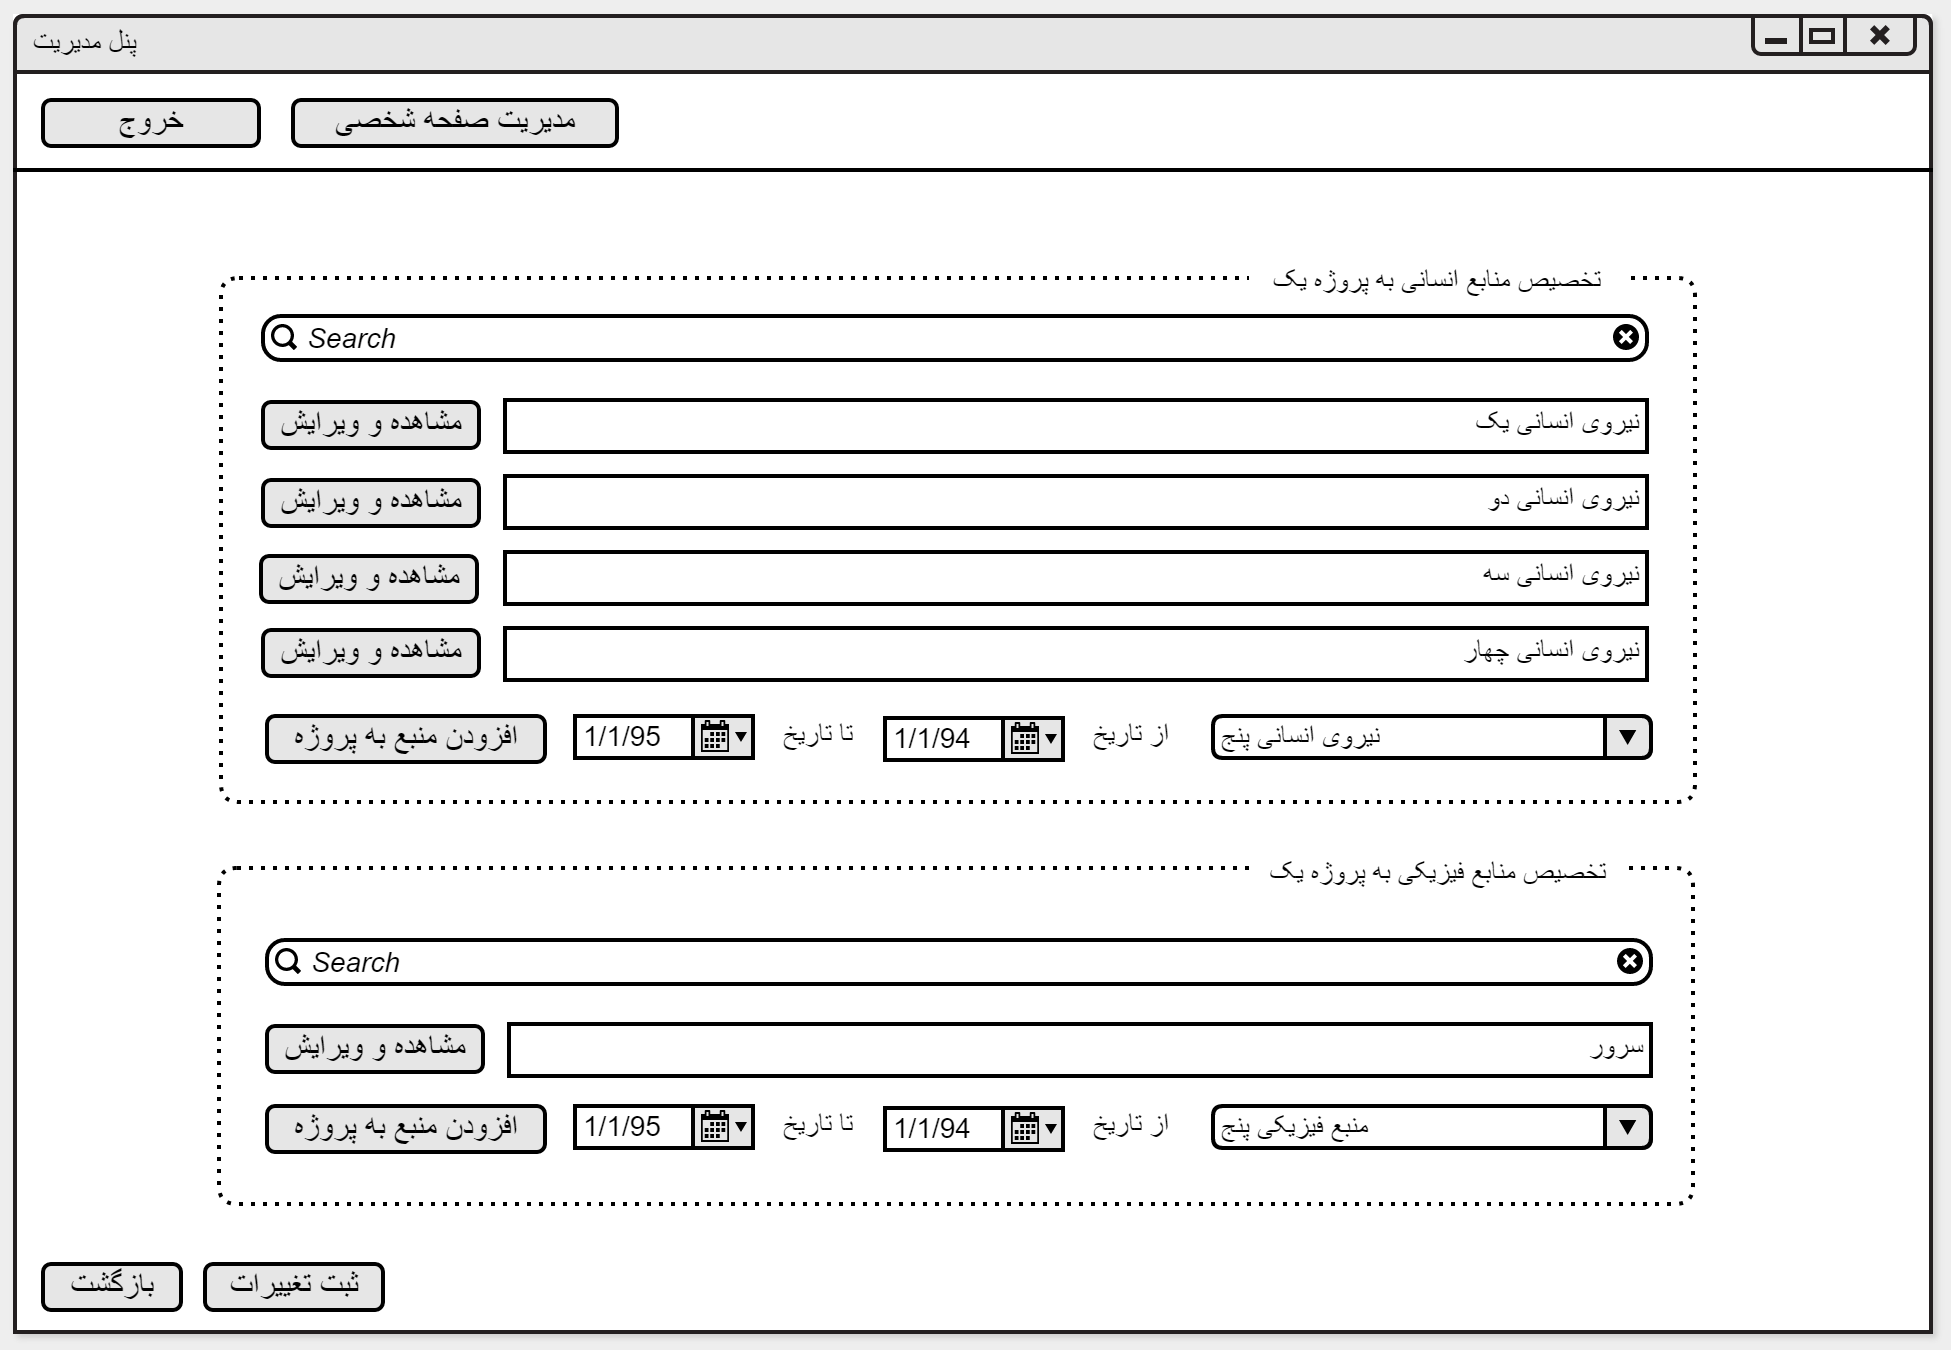
\includegraphics[width=\textwidth]{Prototype/HeadManager/ResourceAssigment.png}
\end{center}

\vspace{1cm}
صفحه‌ی ایجاد پروژه‌ی جدید
\begin{center}
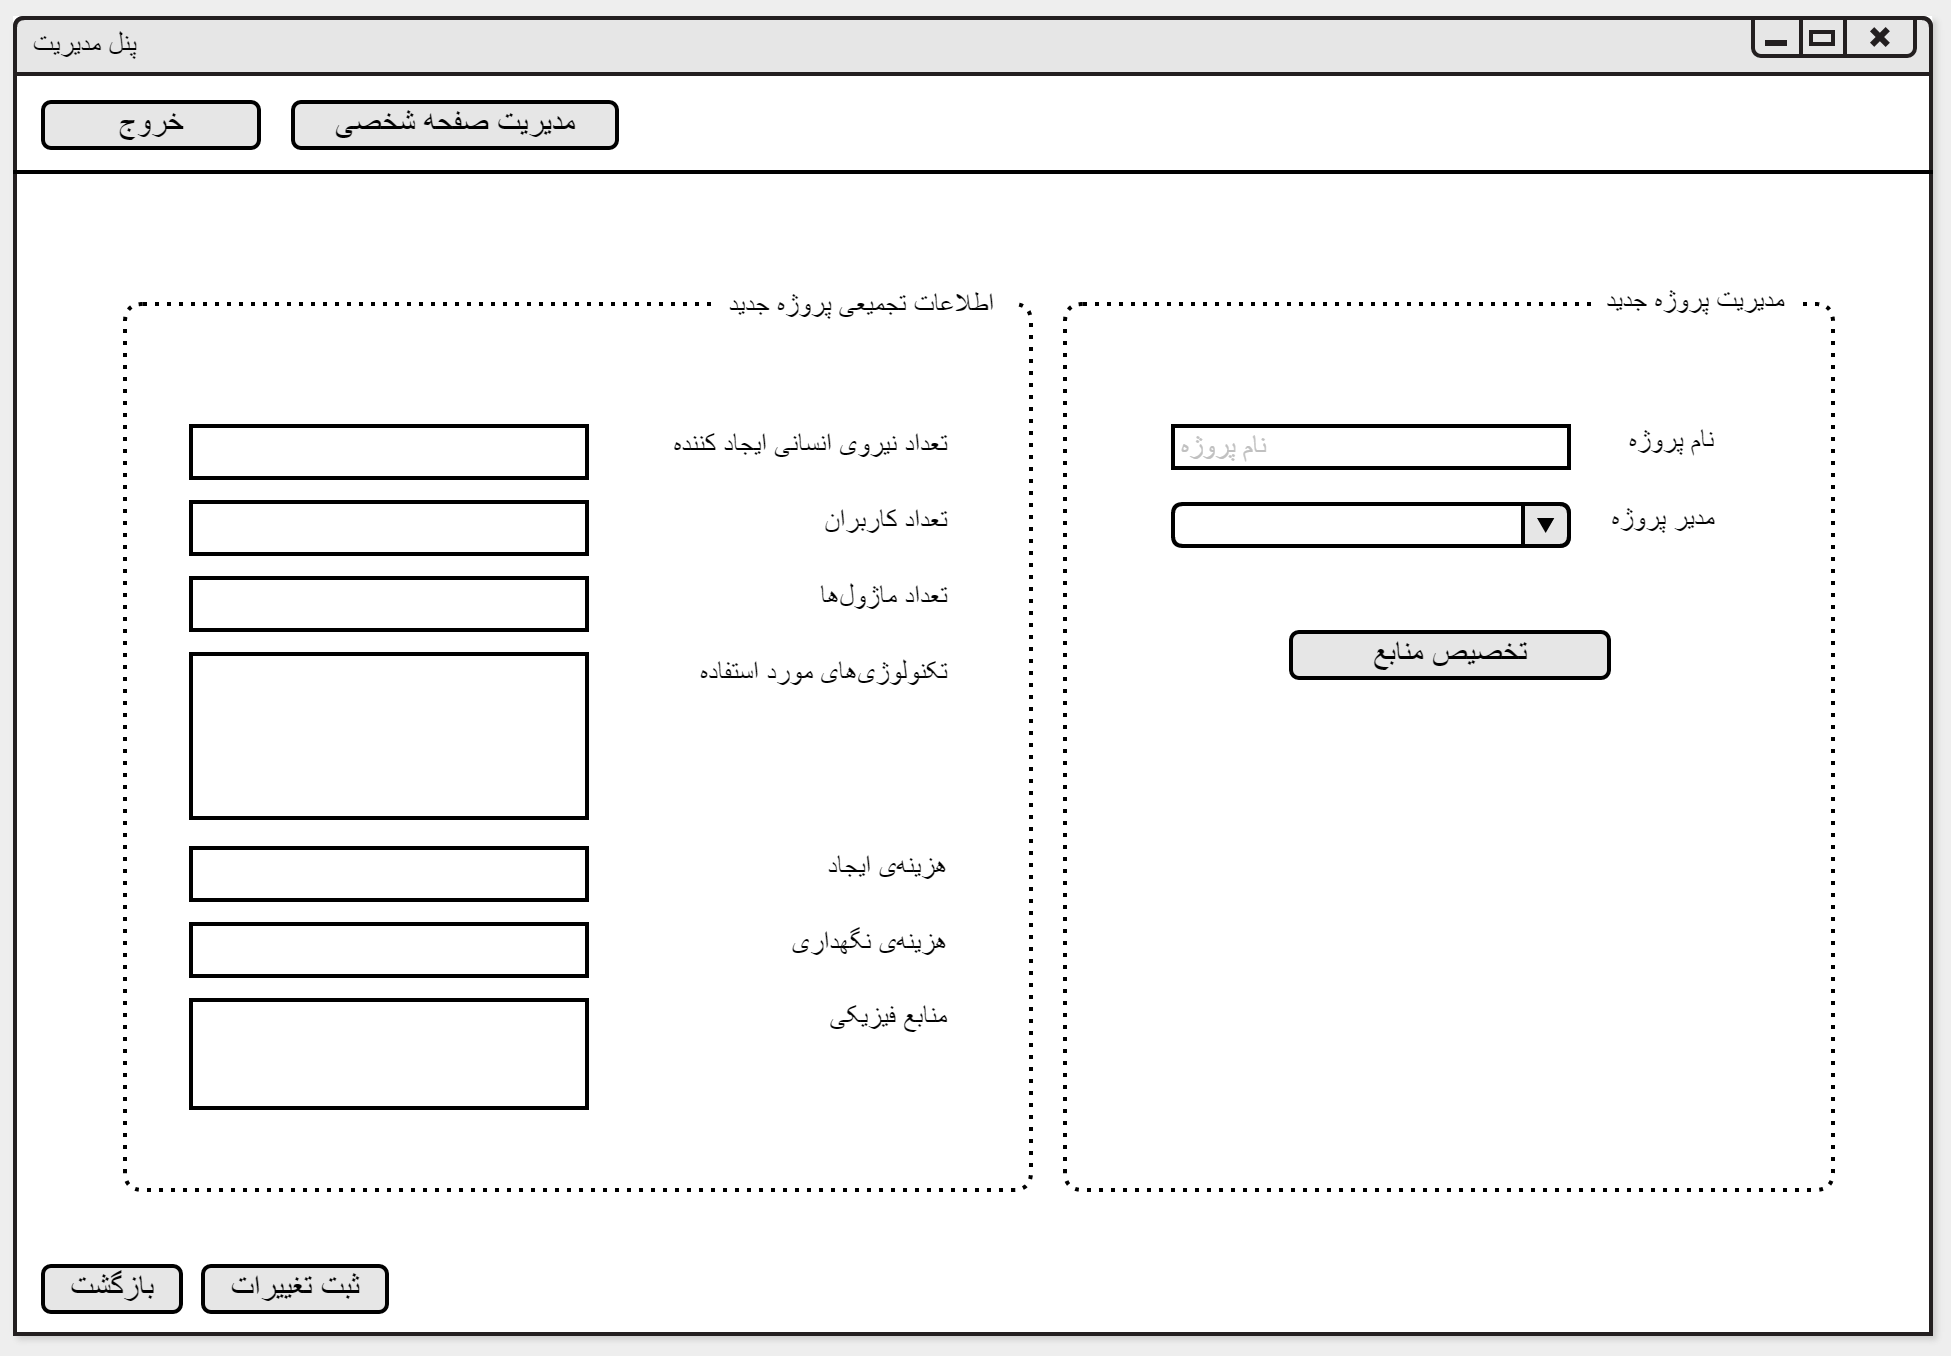
\includegraphics[width=\textwidth]{Prototype/HeadManager/CreateNewProject.png}
\end{center}

\newpage
\vspace{1cm}
صفحه‌ی مدیریت منابع 
\begin{center}
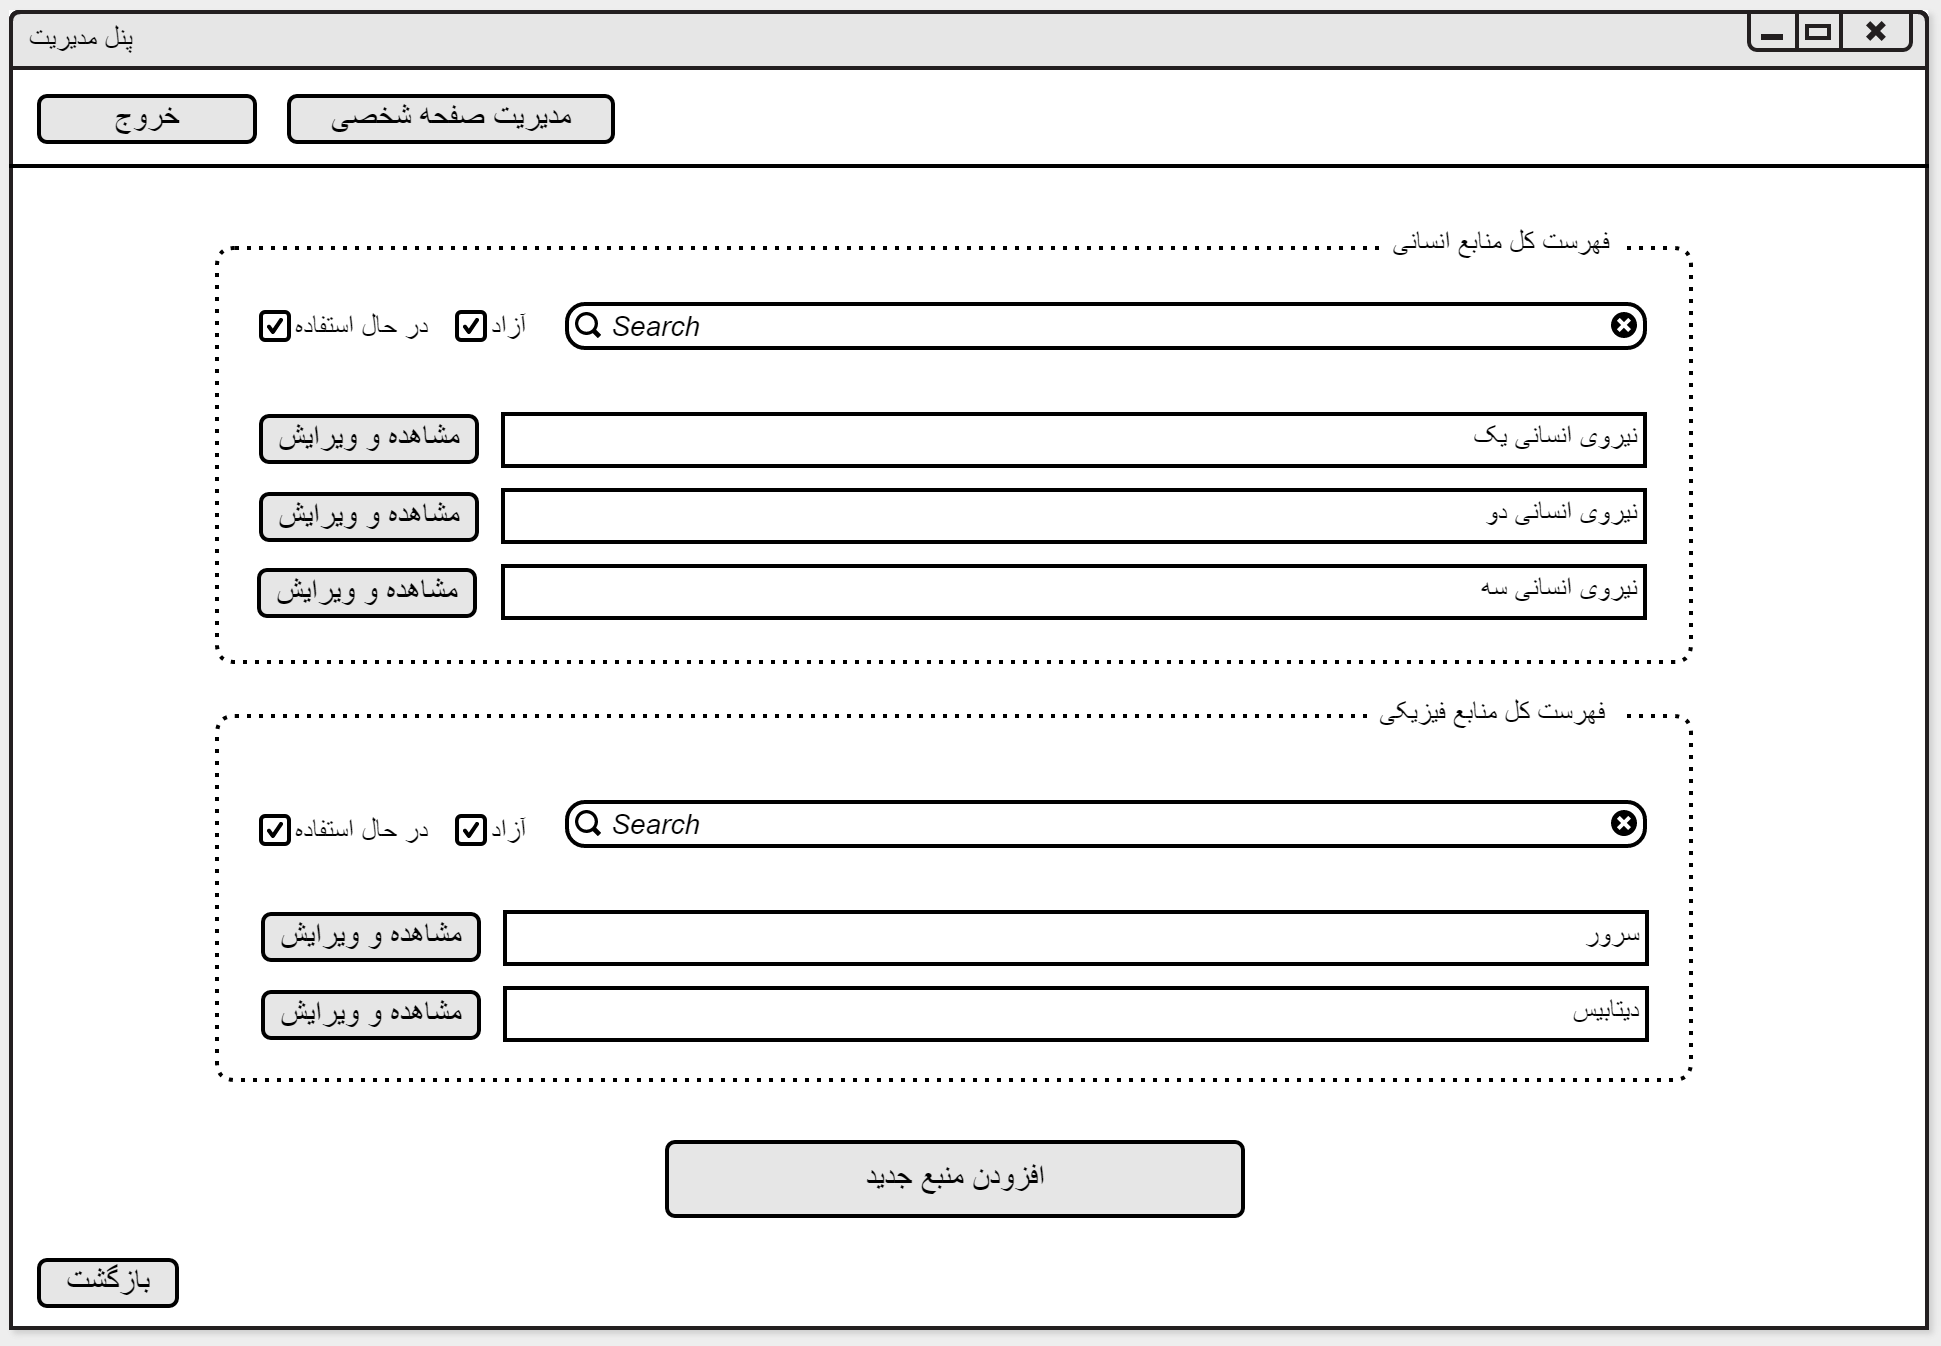
\includegraphics[width=\textwidth]{Prototype/HeadManager/ManageAllResources.png}
\end{center}

\newpage
\subsection{صفحات ابزار گزارش‌گیری}

\vspace{1cm}
صفحه‌ی پنل اصلی ابزار گزارش‌گیری
\begin{center}
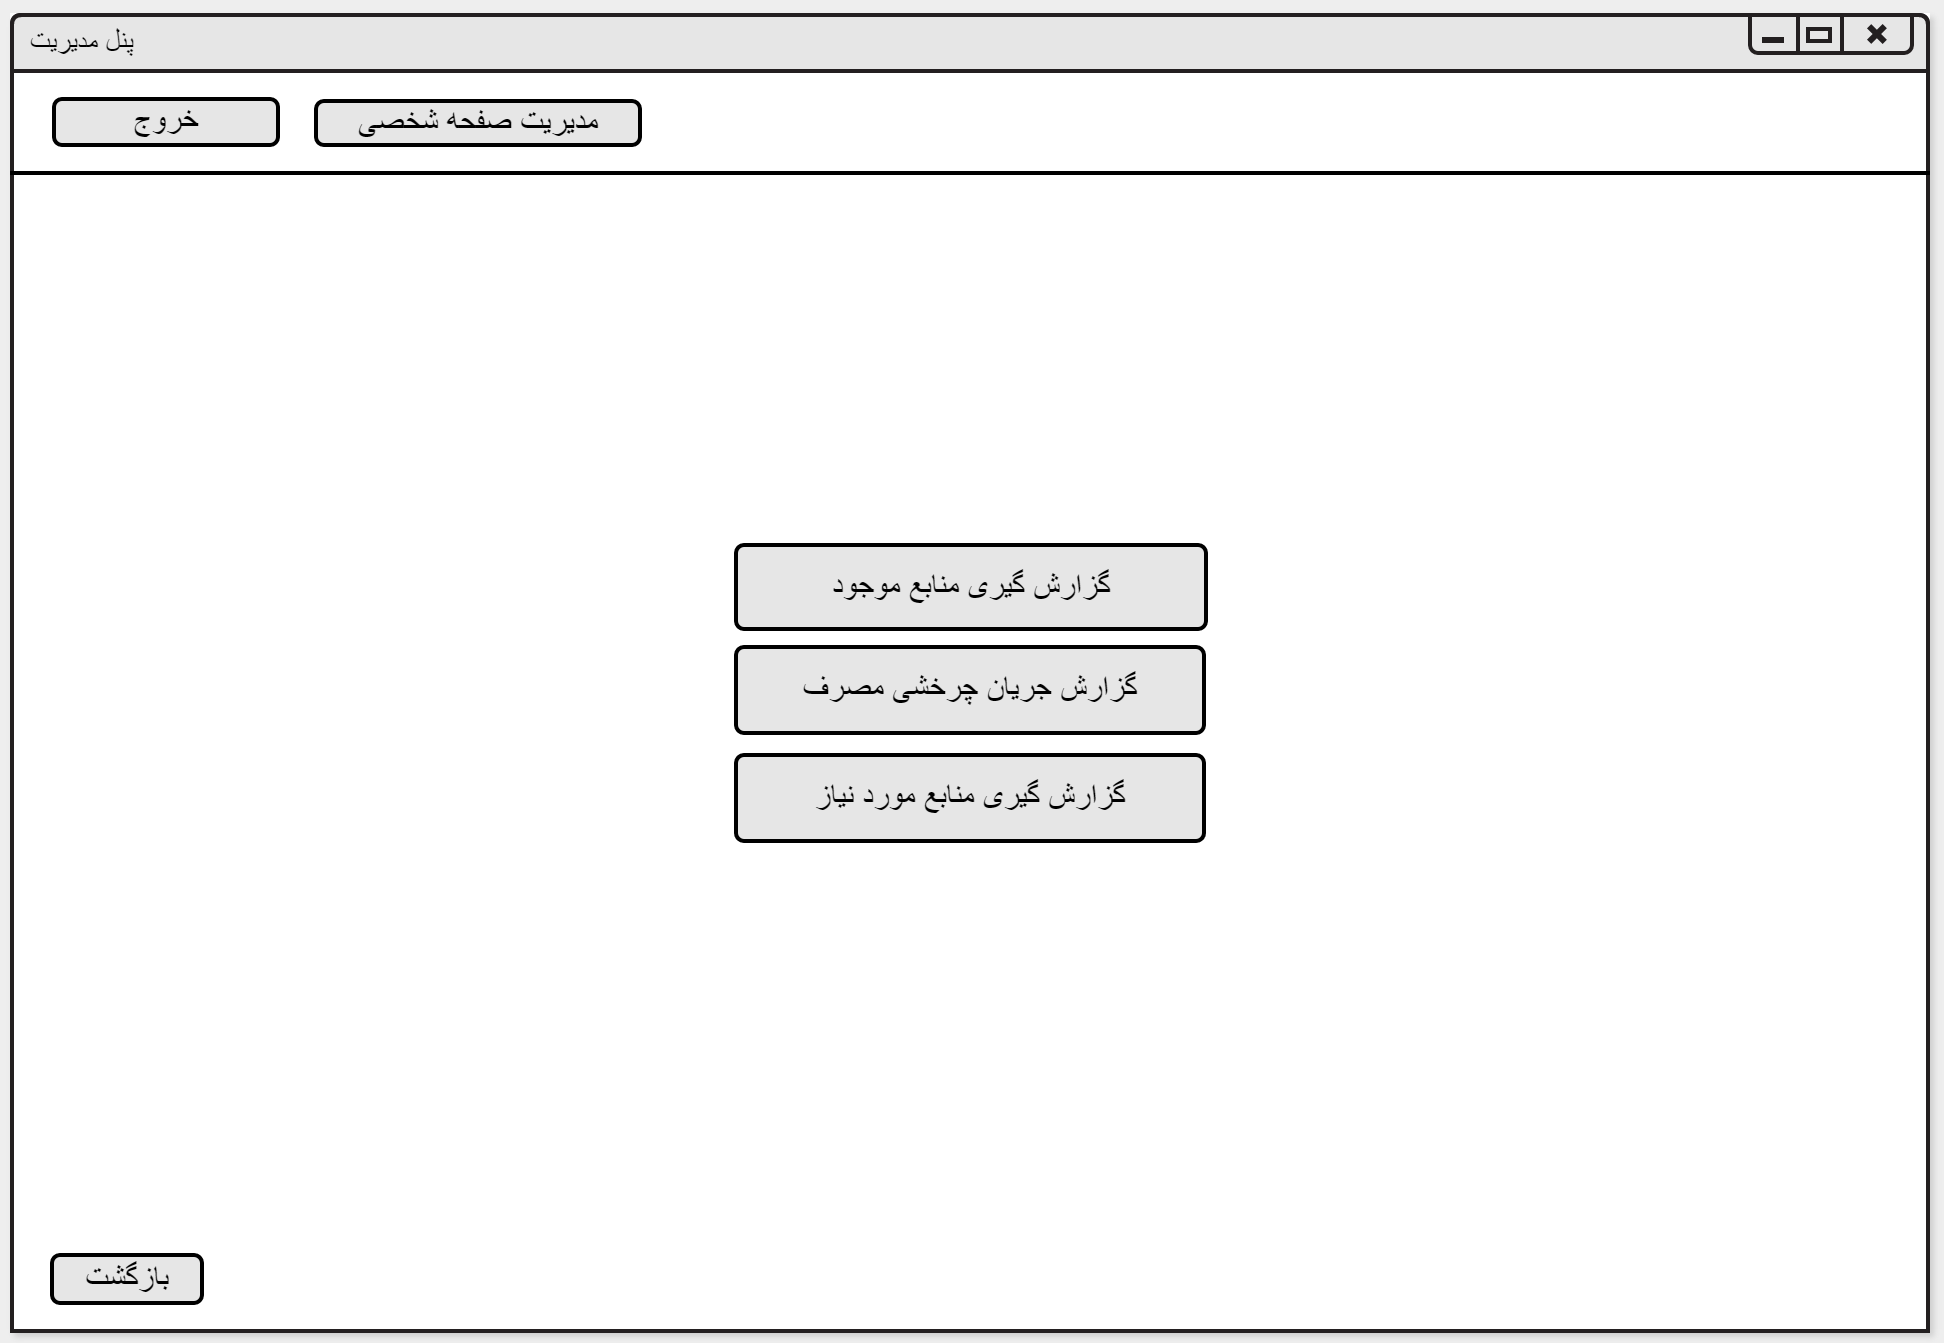
\includegraphics[width=\textwidth]{Prototype/Reporting/ReportHomePage.png}
\end{center}

\newpage
\vspace{1cm}
صفحه‌ی گزارش‌گیری منابع موجود
\begin{center}
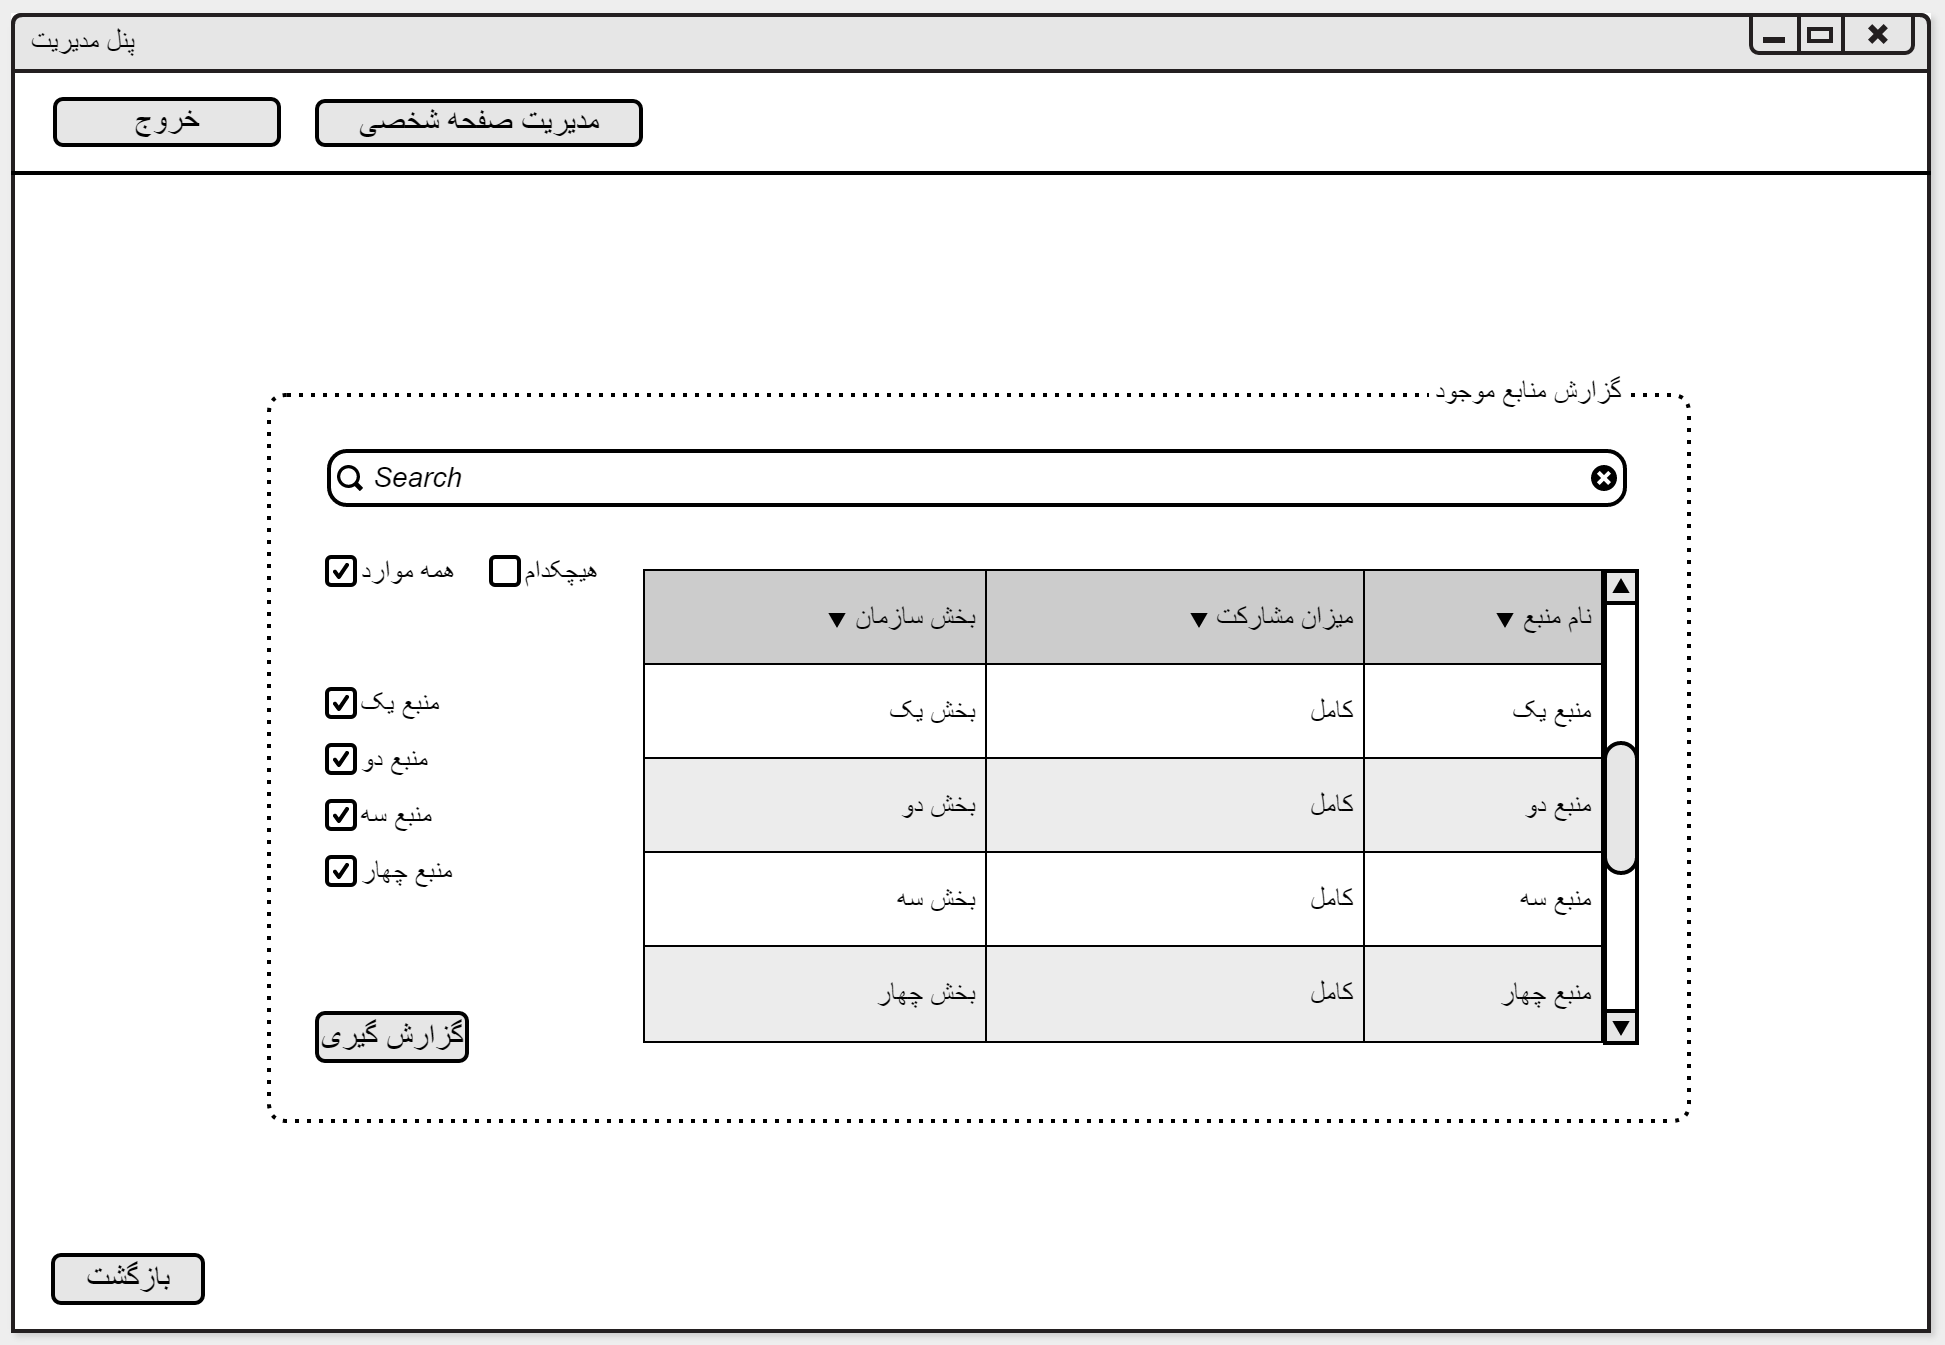
\includegraphics[width=\textwidth]{Prototype/Reporting/ResourceReport.png}
\end{center}

\vspace{1cm}
صفحه‌ی گزارش جریان چرخشی مصرف منابع
\begin{center}
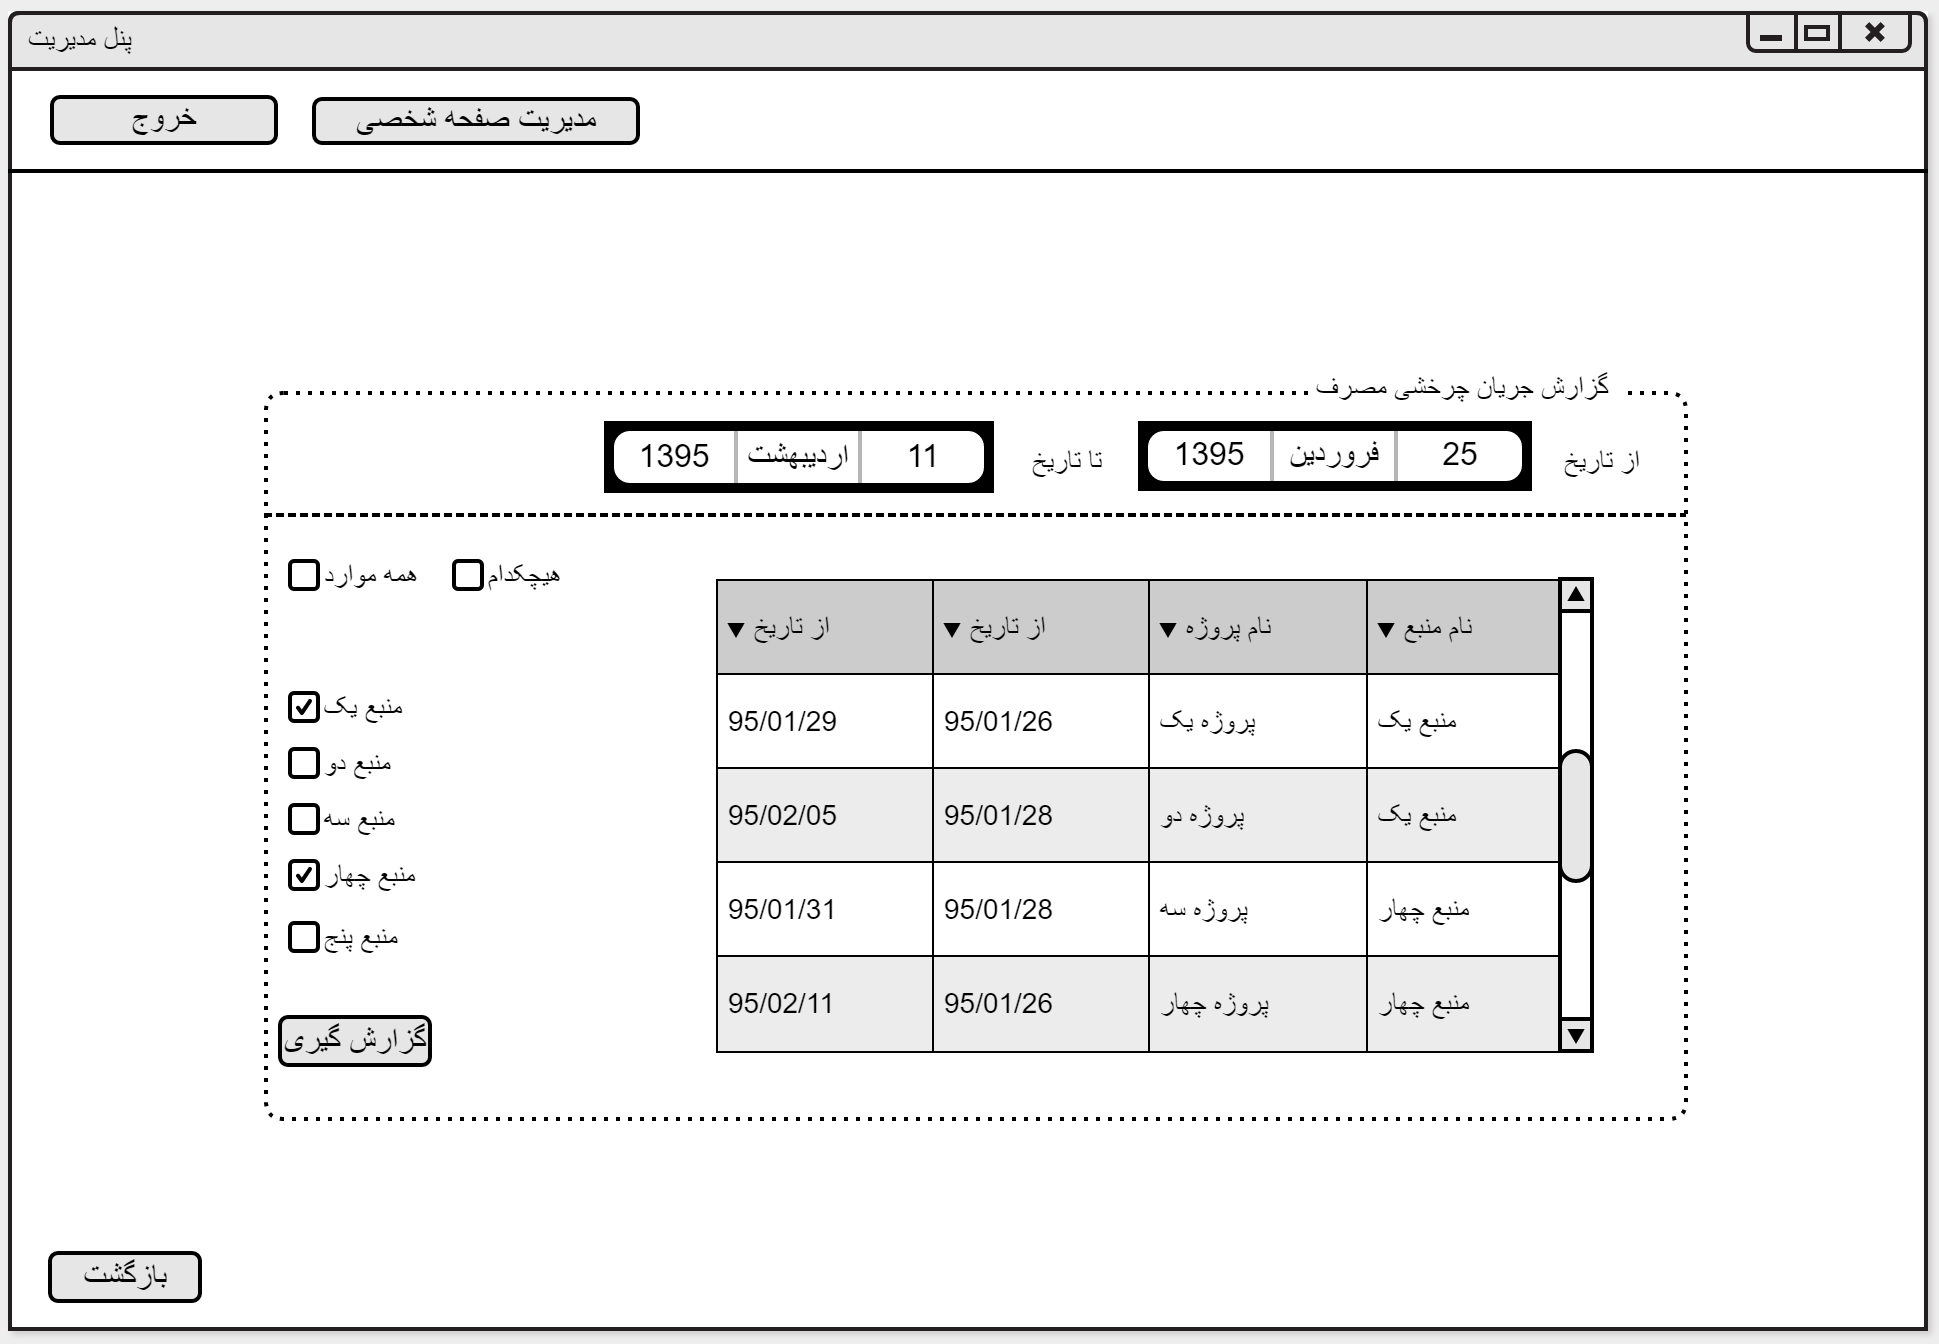
\includegraphics[width=\textwidth]{Prototype/Reporting/ResourceUsageReport.png}
\end{center}

\newpage
\vspace{1cm}
صفحه‌ی گزارش‌گیری منابع مورد نیاز
\begin{center}
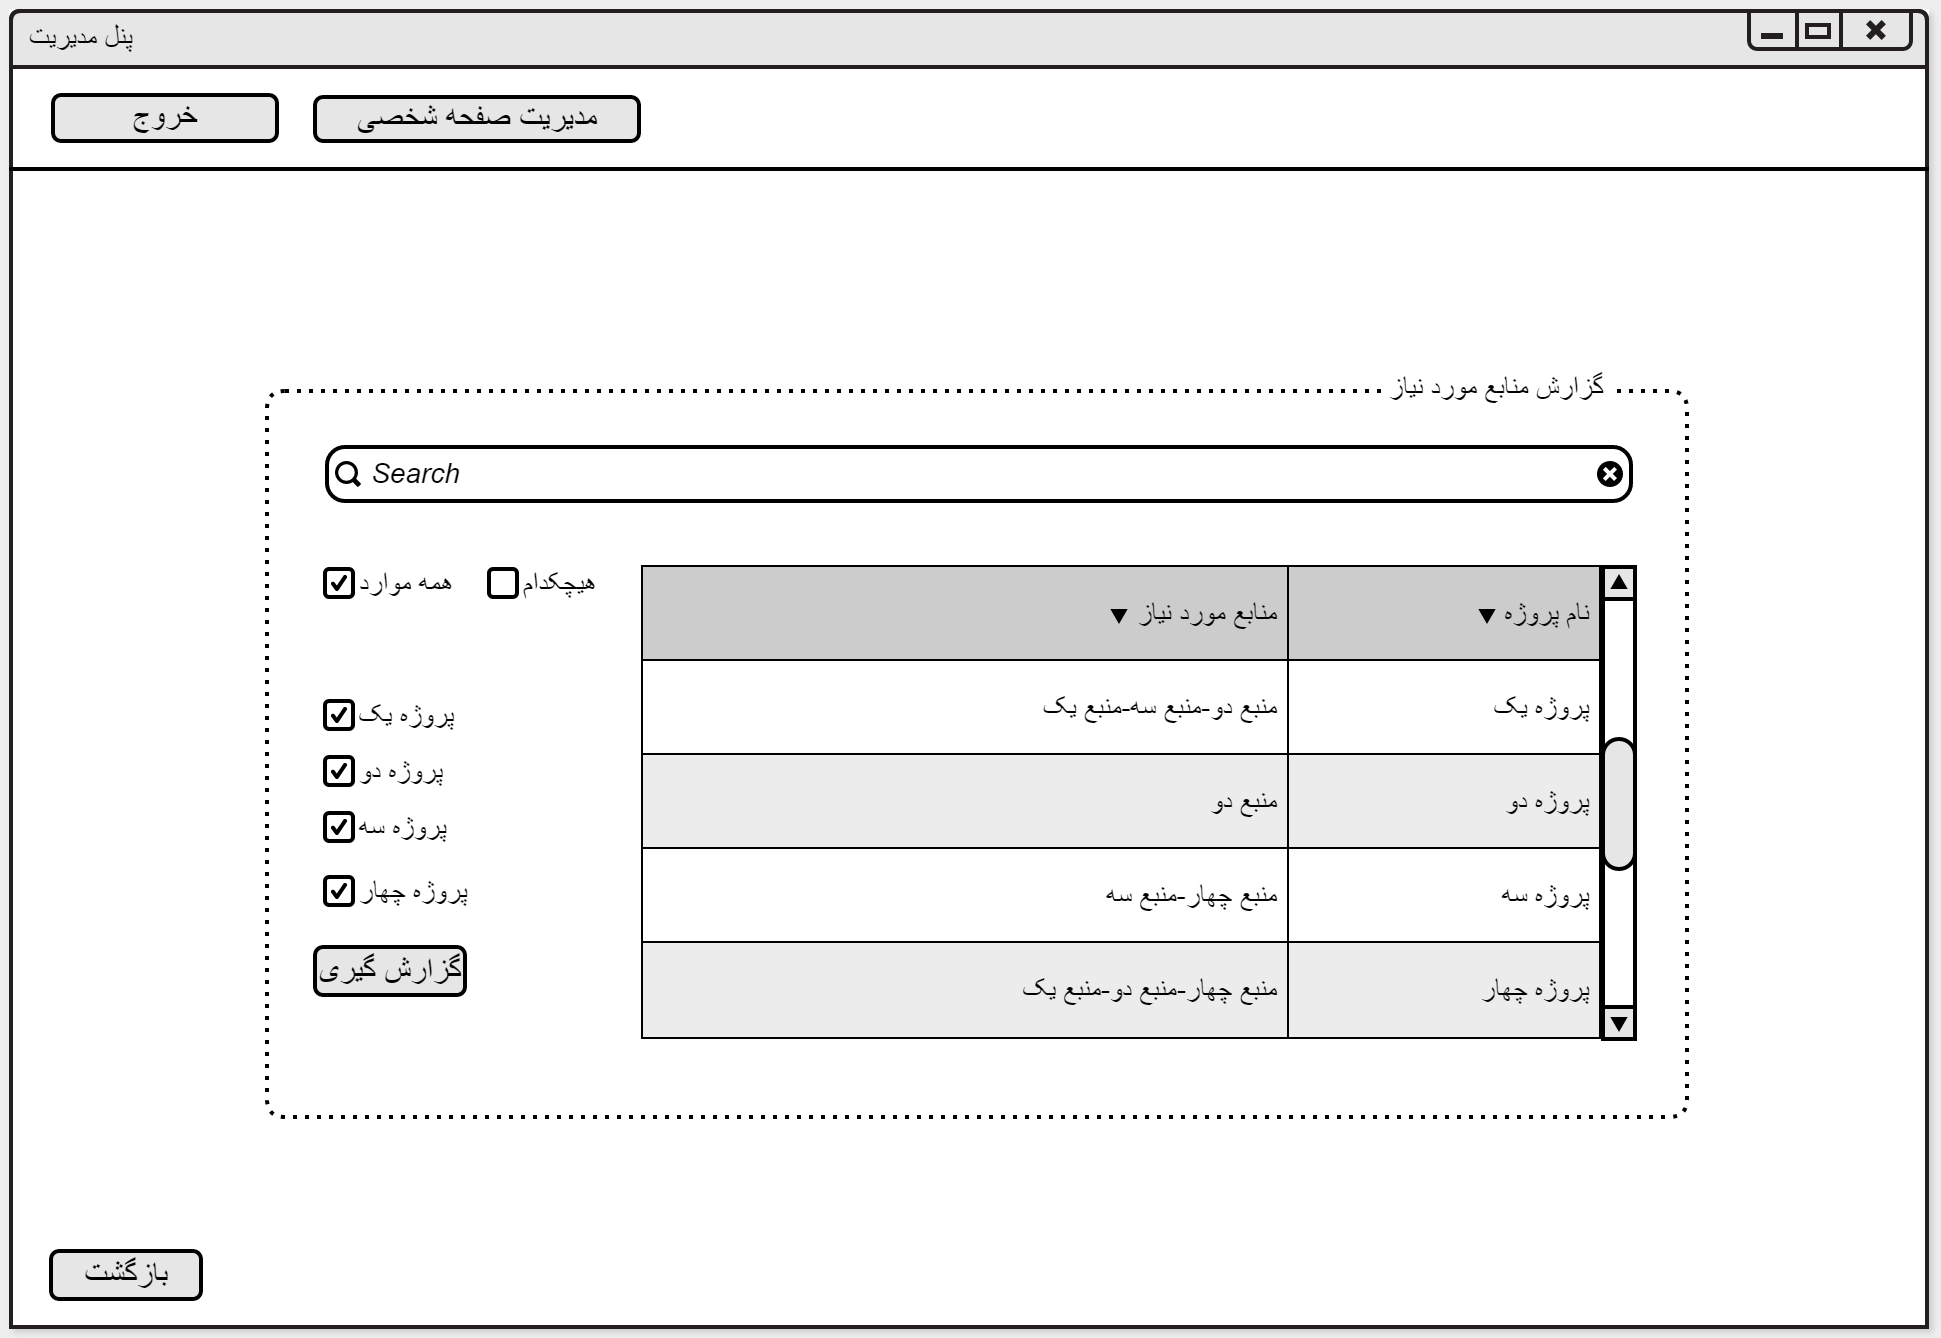
\includegraphics[width=\textwidth]{Prototype/Reporting/ResourceRequirementsReport.png}
\end{center}

\newpage
\subsection{صفحات ابزارپیش‌بینی }

\vspace{1cm}
صفحه‌ی پنل اصلی ابزار پیش‌بینی
\begin{center}
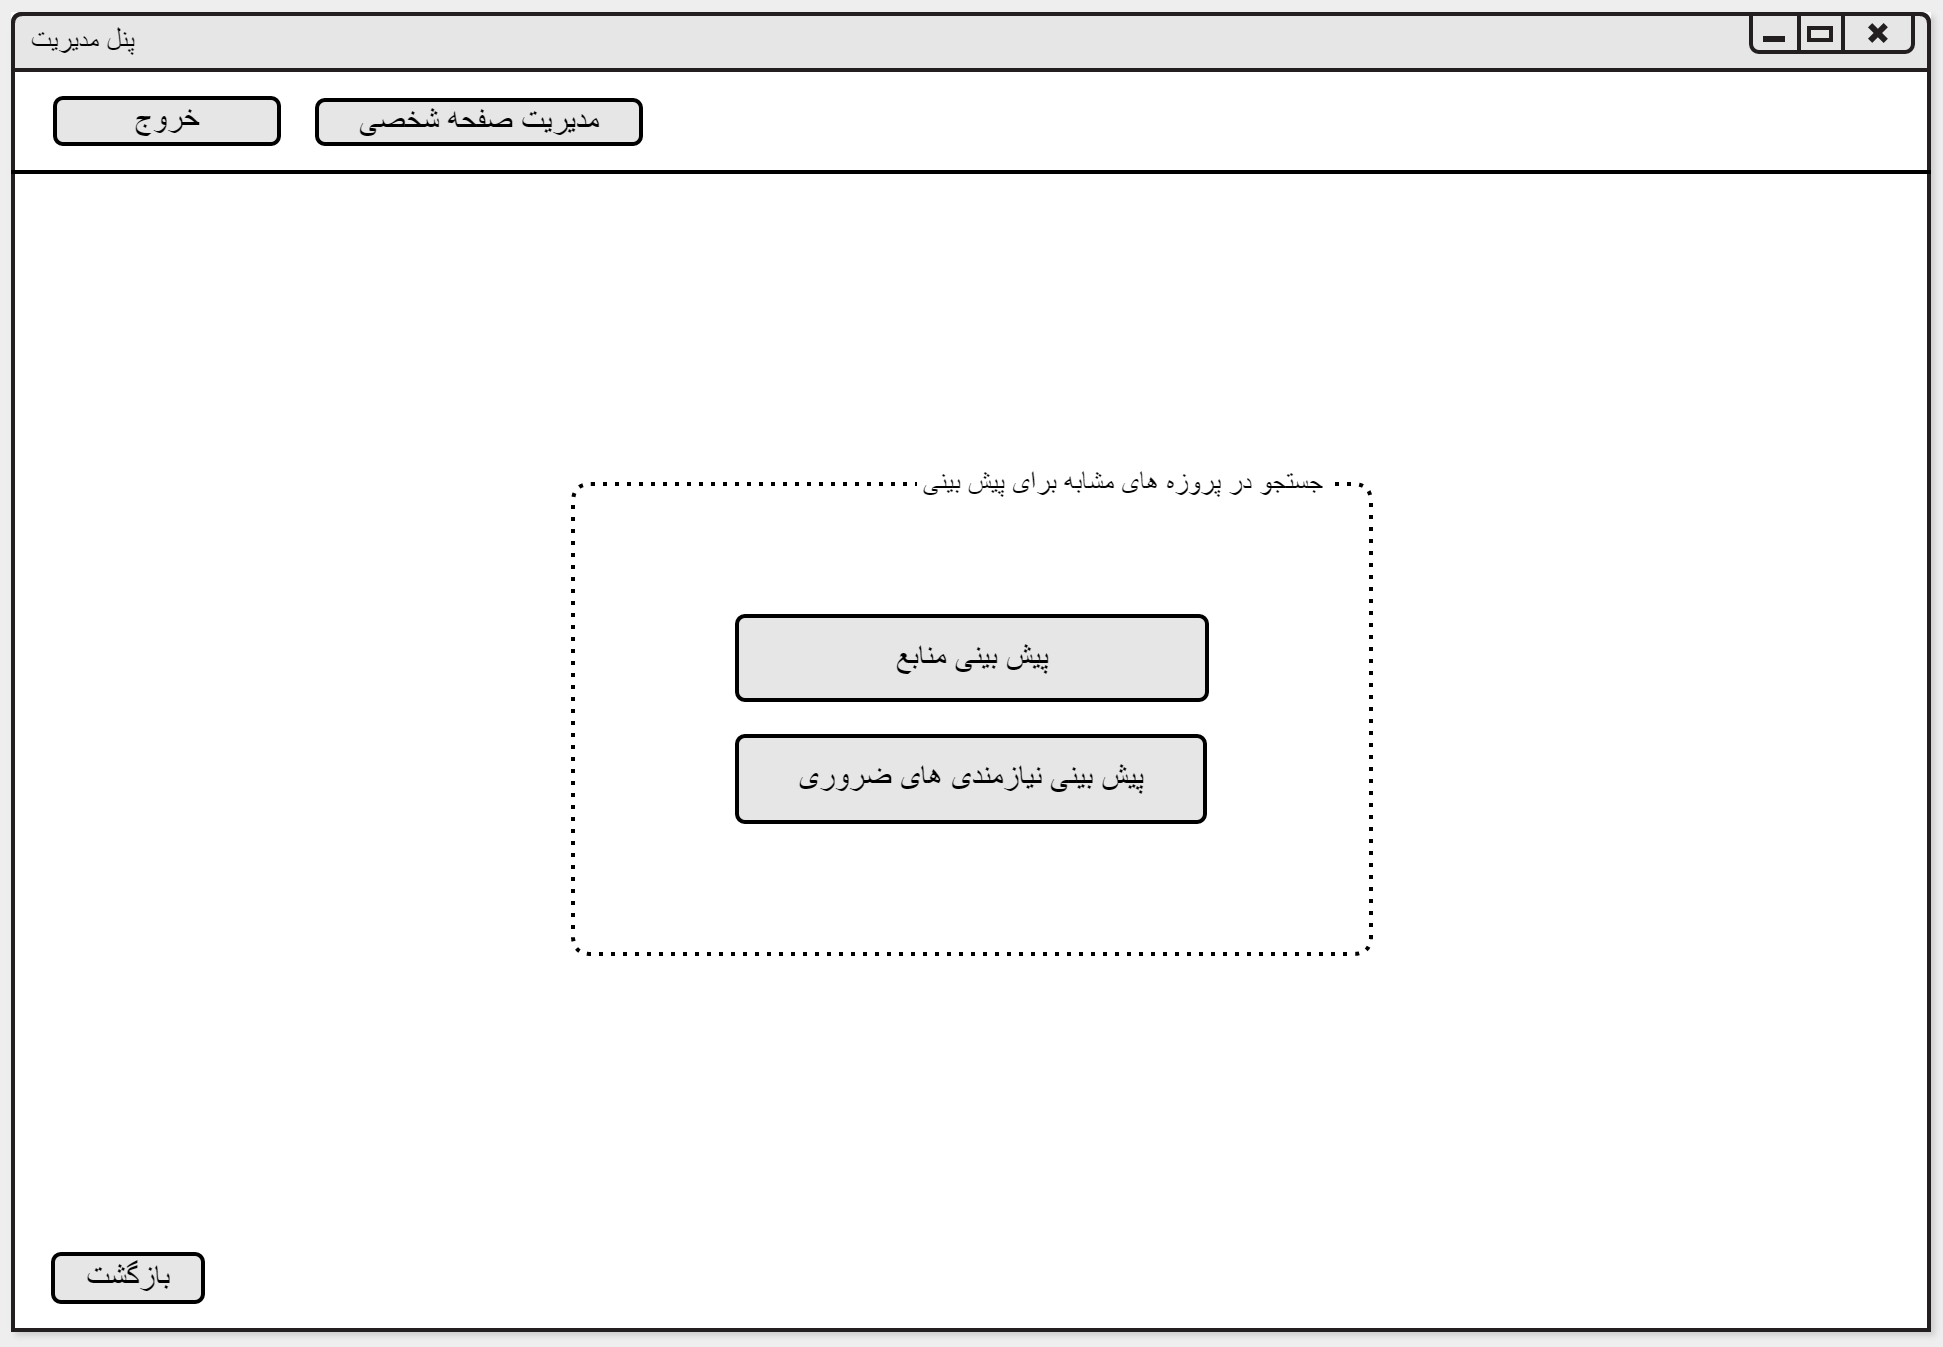
\includegraphics[width=\textwidth]{Prototype/Predict/PredictHomePage.png}
\end{center}

\newpage
\vspace{1cm}
صفحه‌ی پیش‌بینی منابع
\begin{center}
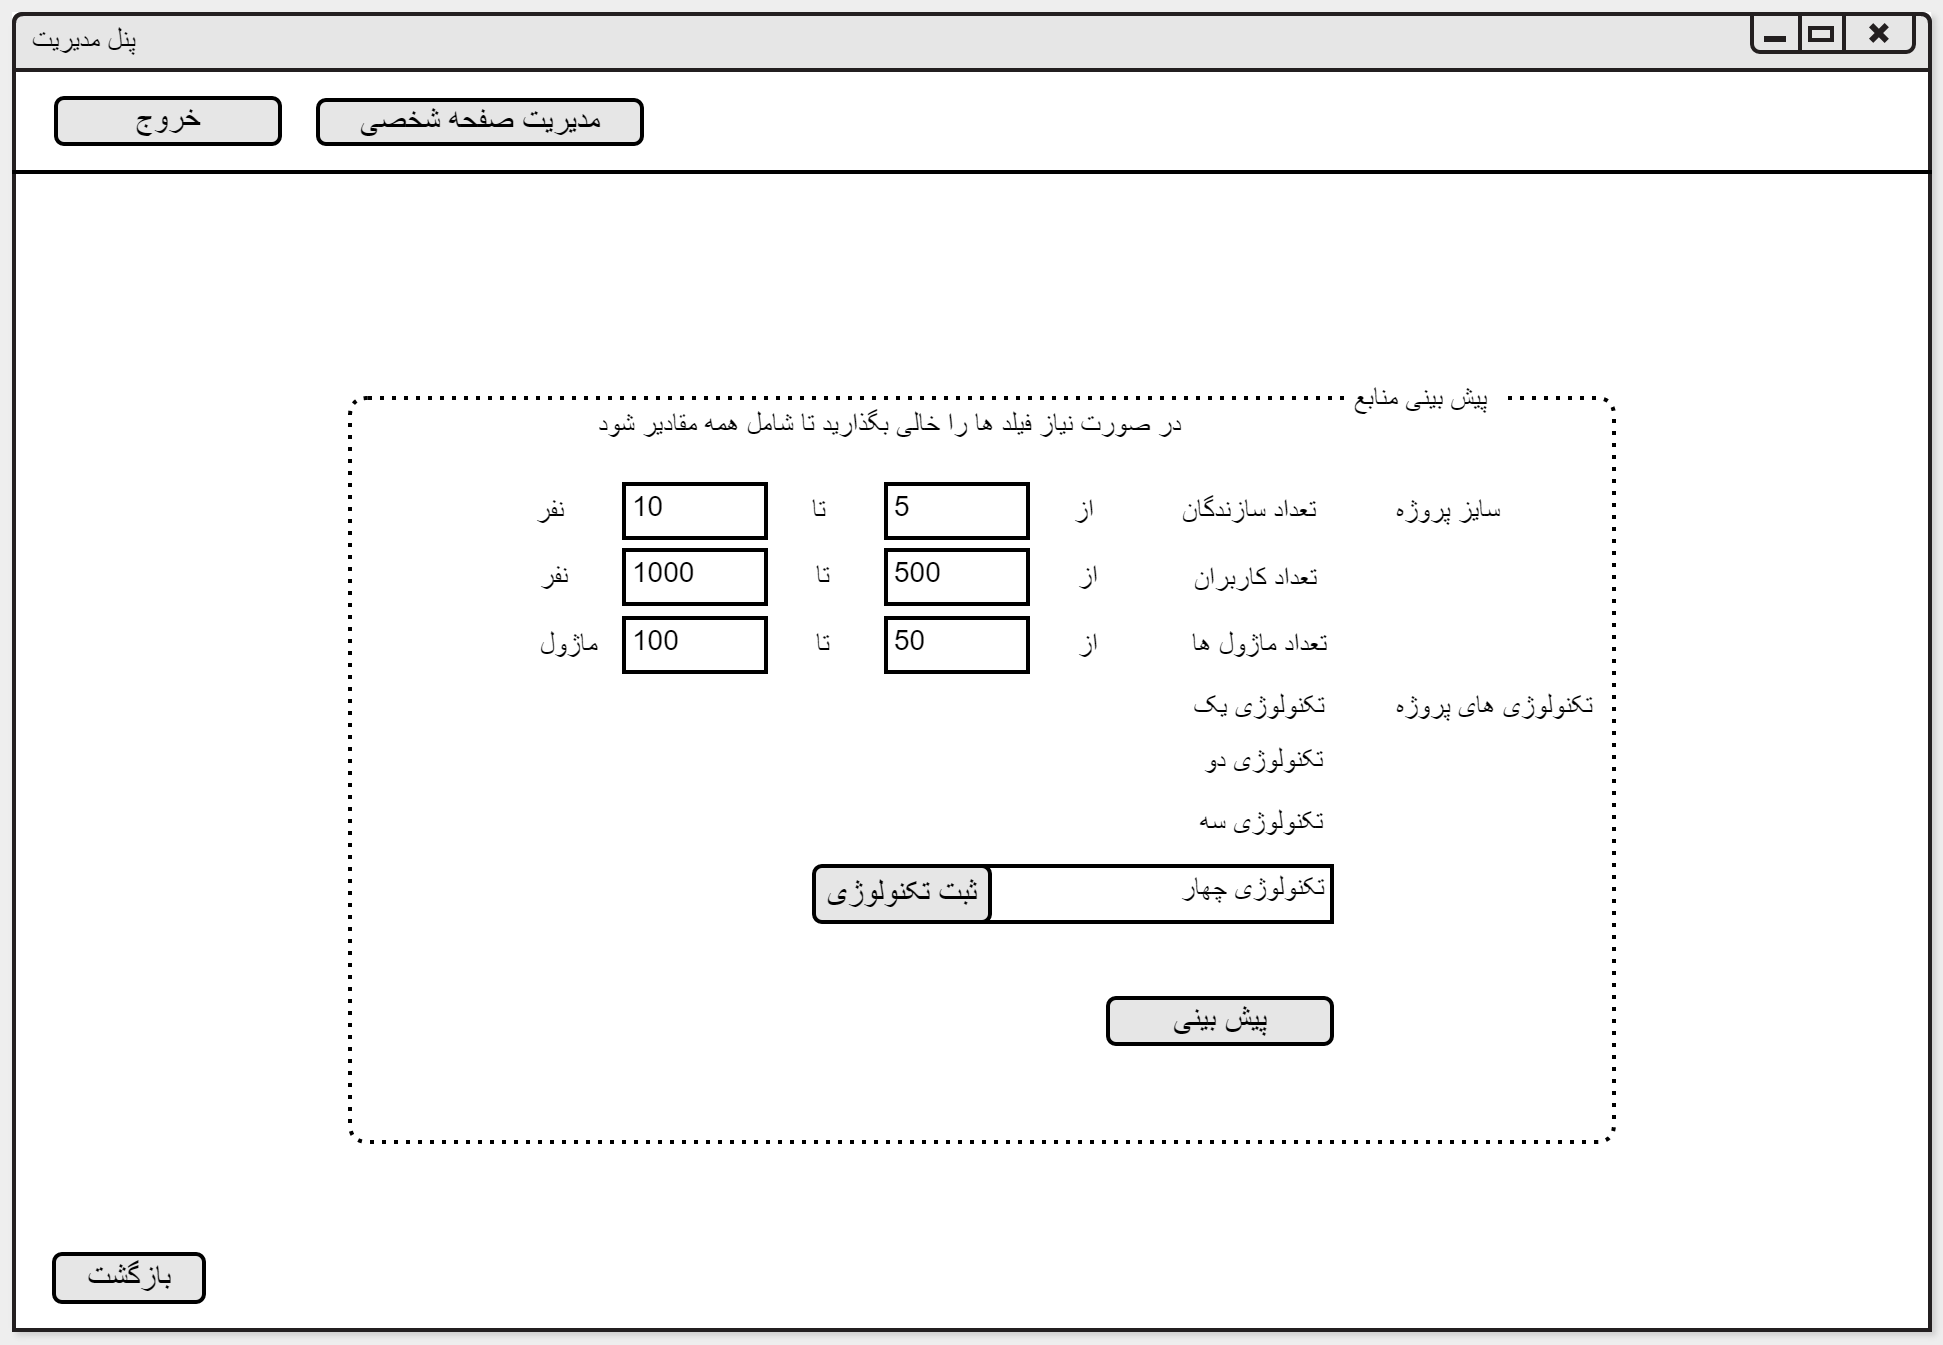
\includegraphics[width=\textwidth]{Prototype/Predict/ResourcePrediction.png}
\end{center}


\vspace{1cm}
صفحه‌ی پیش‌بینی نیازمندی‌های ضروری
\begin{center}
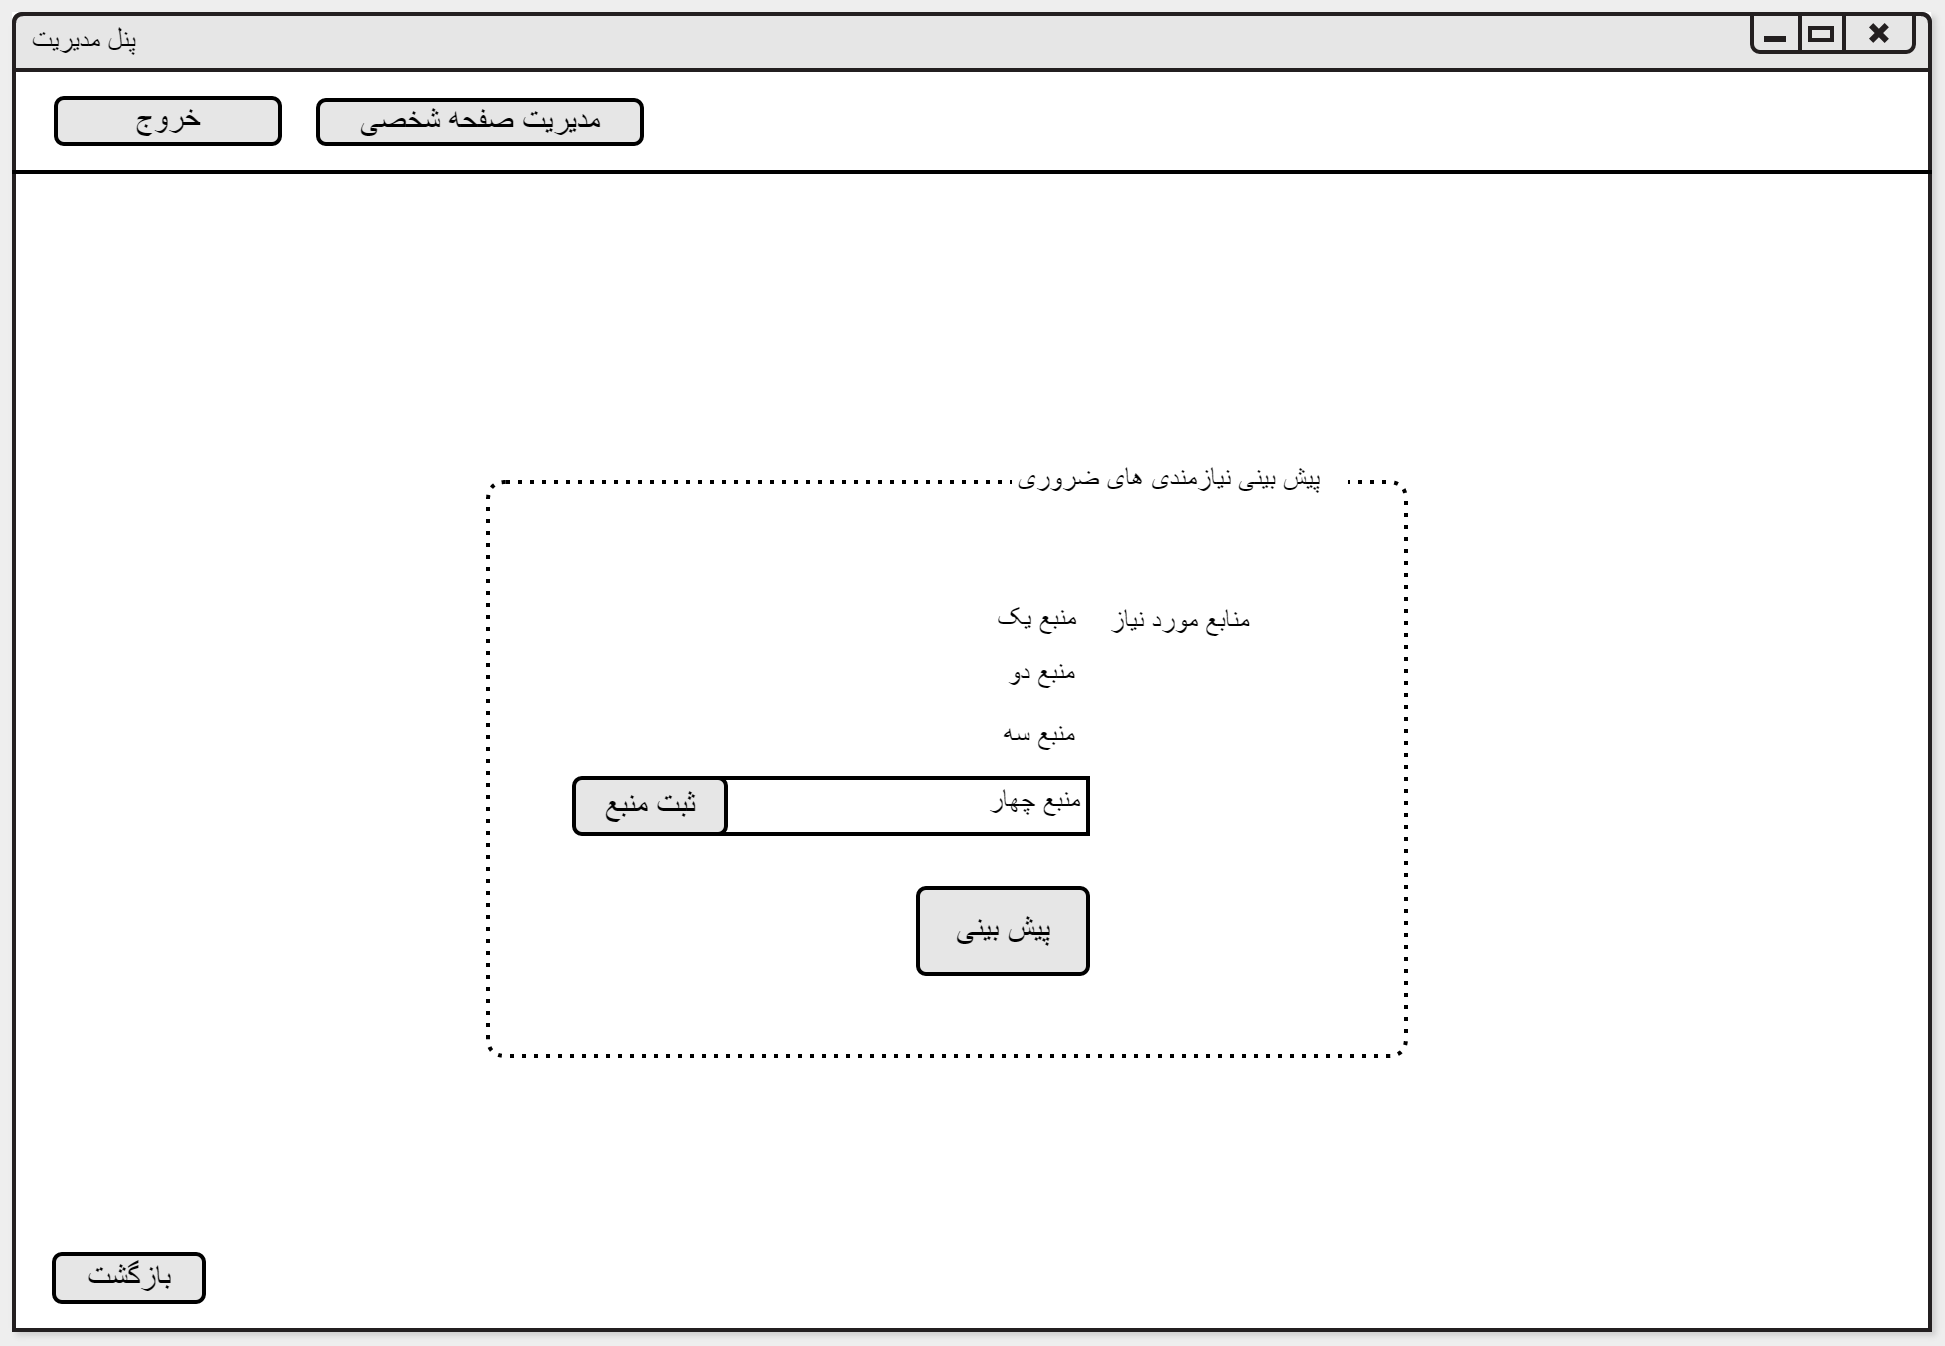
\includegraphics[width=\textwidth]{Prototype/Predict/RequirementsPrediction.png}
\end{center}

\newpage
\vspace{1cm}
صفحه‌ی نتایج پیش‌بینی
\begin{center}
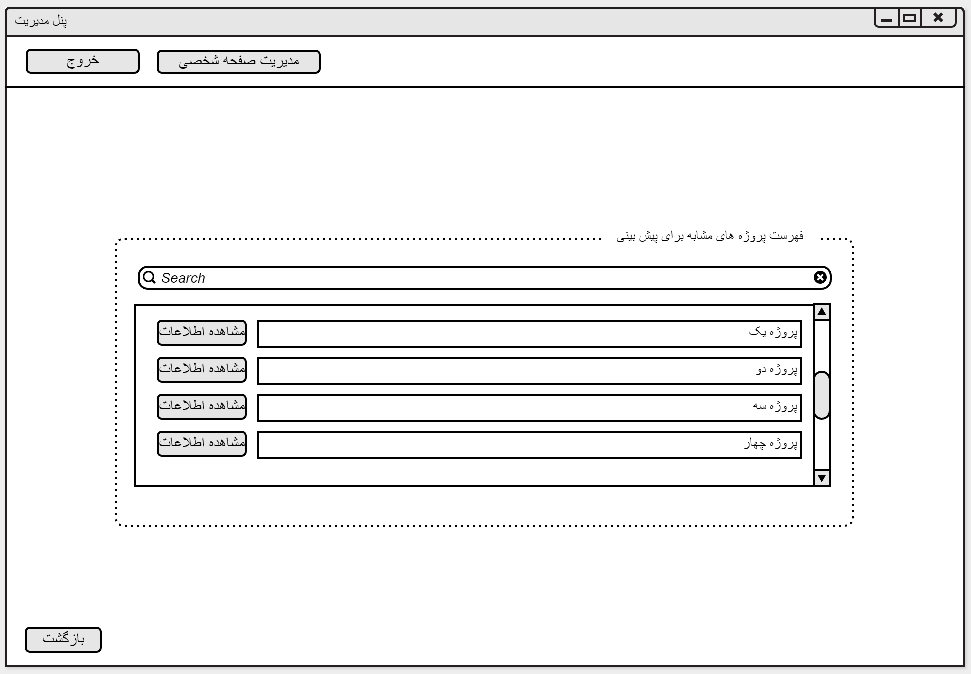
\includegraphics[width=\textwidth]{Prototype/Predict/Result.png}
\end{center}

\newpage
\section{فهرست اولویت‌بندی شده‌ی ریسک‌ها}

\subsection{درک نادرست از خواسته‌های پروژه}
\begin{itemize}
\item توصیف: این ریسک زمانی مطرح است که مشتری و سازندگان در فهم منظور یکدیگر با خطا مواجه شوند. ممکن است این اتفاق به دلیل واضح نبودن یا ابهام داشتن خواسته های مشتری، و یا ناشی از کمبود اطلاعات سازندگان از حوزه‌ی مسئله باشد. این بدین معنی است که هر دو طرف می‌توانند در این ریسک سهم داشته باشند. درک نادرست از خواسته‌های پروژه، در نهایت منجر به ارائه‌ی محصولی می‌شود که با محصول مورد نظر مشتری متفاوت است. به عنوان مثال، ممکن است سازندگان در مورد اولویت نیازمندی‌ها از طرف مشتری دچار اشتباه شوند و به جنبه‌های کم‌اهمیت‌تر بپردازند. اگر به اندازه‌ی کافی وقت و انرژی صرف کنترل این ریسک نشود، این ریسک می‌تواند مستقیما به شکست پروژه بیانجامد.
\item احتمال وقوع: بالا
\item احتمال شکست: بالا
\item راه حل: برای رفع این مشکل باید در ضمن قرارداد، تمامی نیازهای وظیفه‌مندی و غیروظیفه‌مندی را ذکر و اولویت آن‌ها را به صورت کامل مشخص کرد تا هرگونه ابهام برای طرفین رفع شود. همچنین می‌توان برای اطمینان از متوجه شدن منظور مشتری، یک نمونه پروتوتایپ به مشتری ارائه کرد و نظر او را در مورد بخش‌های مختلف و ارتباط زیربخش‌ها با یکدیگر پرسید.
\end{itemize}

\subsection{مشکل در برقراری ارتباط با مشتری}
\begin{itemize}
\item توصیف: در صورتی که راهی برای برقراری ارتباط مداوم با مشتری و پرسیدن سوالات در نظر گرفته نشده باشد، این ریسک مطرح می‌شود. از نتایج وقوع این ریسک می‌توان به دوباره‌کاری‌ها و اتلاف هزینه‌های مالی و زمانی اشاره کرد. چرا که عدم ارتباط مداوم موجب می‌شود که سازندگان با توجه به پیش‌فرض‌ها و برداشت‌های خود در مورد مسائل مختلف مرتبط به پروژه تصمیم‌گیری کنند.
\item احتمال وقوع: بالا
\item احتمال شکست: متوسط
\item راه حل: بهترین و مطمئن‌ترین راه‌حل برای کنترل این ریسک، حضور دائمی یک عضو از تیم مشتریان در تیم سازندگان است. در این صورت احتمال سوءبرداشت‌ها کاهش می‌یابد و اگر شبهه‌ای در مسیر انجام پروژه پیش بیاید، با صرف زمان حداقلی رفع می‌شود. اگر این راه میسر نبود، توصیه می‌شود که راهی برای ارتباط سریع و آسان در هنگام بروز مشکل وجود داشته باشد، و جلسات هفتگی یا ماهیانه برای بررسی مسیر پروژه برگزار شود.
\end{itemize}


\subsection{مقاومت کاربران}
\begin{itemize}
\item توصیف: عموما کاربران در مقابل هرگونه تغییر در روش انجام فعالیت‌ها از خود مقاومت نشان می‌دهند. کاربران این سامانه پس از اتمام مراحل راه‌اندازی، موظف می‌شوند که اطلاعات مربوطه را در سامانه وارد کنند. پس احتمال دارد که در ابتدای امر با مقاومت از سوی کاربران مواجه شویم و آزمون پذیرش نتیجه‌ی منفی داشته باشد. اما چون این یک ریسک معمول در میان پروژه‌هایی از این نوع است، احتمال شکست پروژه زیاد نیست.
\item احتمال وقوع: بالا
\item احتمال شکست پروژه: متوسط
\item راه حل: آموزش صحیح کاربران و تفهیم اهمیت انجام این پروژه و فوایدی که در پی خواهد داشت.
\end{itemize}

\subsection{اختلاف در معیارهای موفقیت پروژه}
\begin{itemize}
\item توصیف: ممکن است معیارهای ارزیابی موفقیت پروژه از دیدگاه مشتری و دیدگاه سازندگان پروژه متفاوت باشد. این امر می‌تواند زیان جبران‌ناپذیری را موجب شود؛ چرا که اگر در زمان انجام مراحل اولیه‌ی پروژه به اندازه‌ی کافی به این مسئله توجه نشود، جبران اشتباهات و تغییر مسیر در مراحل بعدی بسیار سخت و شاید غیرممکن خواهد بود.
\item احتمال وقوع: بالا
\item احتمال شکست پروژه: متوسط
\item راه حل: برای رفع این مشکل می‌توان در ضمن قرارداد همه‌ی معیارهای شکست و موفقیت را به درستی و بدون ابهام ذکر کرد. تعریف دقیق پروژه‌ی کامل و موفق، می‌تواند این ریسک را به خوبی کنترل کند. این تعریف باید شامل تمامی معیارهای نهایی ارزیابی پروژه باشد. توصیه می‌شود که در صورت امکان برای هریک از نیازمندی‌ها، معیار کمّی متناسب با آن ذکر شود. بدین ترتیب، احتمال وقوع این ریسک به حداقل می‌رسد.
\end{itemize}


\subsection{کمبود زمان}
\begin{itemize}
\item توصیف: به علت فشردگی زمان‌بندی برای انجام این پروژه و این که تیم سازنده نمی‌تواند به صورت تمام‌وقت به انجام پروژه بپردازد، ریسک نرسیدن به زمان‌بندی وجود دارد.
\item احتمال وقوع: کم
\item احتمال شکست: متوسط
\item راه حل: پرداختن به نیازمندی‌های ضروری پروژه و اولویت‌بندی دقیق آن‌ها، می‌تواند نقش قابل توجهی در راستای رفع این ریسک داشته باشد. همچنین به دلیل این که در زمان بندی پیش‌بینی شده، تیم سازنده در فاز پیاده‌سازی می تواند وقت بیشتری را به انجام این پروژه اختصاص دهد، این ریسک قابل کنترل است.
\end{itemize}

\subsection{تغییر نیازمندی‌ها}
\begin{itemize}
\item توصیف: ممکن است مشتری در طول انجام پروژه، به دلیل تغییر شرایط کاری، شناخت بهتر مسئله و یا دلایل دیگر، نیازمندی‌های خود را تغییر دهد. اگر این تغییرات محدود و در راستای مسیر کنونی پروژه باشد، مشکلی در ادامه‌ی پروژه رخ نخواهد داد. اما اگر نیازمندی‌های جدید با نیازمندی‌های کنونی مغایرت داشته باشد و یا مسیر اصلی پروژه را تغییر دهد، احتمال شکست پروژه و یا حداقل ایجاد هزینه‌های سنگین برای ادامه‌ی پروژه بالا می‌رود.
\item احتمال وقوع: متوسط
\item احتمال شکست:بالا
\item راه حل: می‌توان وظایف و چارچوب اصلی پروژه را در قرارداد ذکر کرد، تا در صورت بروز اختلاف، نیازمندی‌های جدید را با آن مطابقت داد. همچنین توصیه می‌شود در قرارداد سقفی برای تغییر نیازمندی‌ها و افزودن نیازمندی جدید در نظر گرفته شود. 
\end{itemize}


\subsection{کمبود منابع (تخمین نادرست از منابع مورد نیاز)}
\begin{itemize}
\item توصیف: عوامل مختلفی مانند درک نادرست از ابعاد پروژه و عدم پیش‌بینی موانع انجام پروژه، می‌تواند گروه سازنده را در تخمین منابع (اعم از منابع انسانی، فیزیکی و مالی) به اشتباه بیاندازد. نتیجه‌ی این اشتباه عموما در نرسیدن به زمان‌بندی پیش‌بینی شده نمایان می‌شود.
\item احتمال وقوع: متوسط
\item احتمال شکست: متوسط
\item راه حل: برای رفع این ریسک می‌توان دو رویکرد در نظر گرفت. رویکرد نخست این که زمان بیشتری را برای بررسی منابع مورد نیاز اختصاص بدهیم تا احتمال وقوع این ریسک کاهش یابد. برای تخمین دقیق‌تر، می توان از اطلاعات پروژه‌های مشابه استفاده کرد.
رویکرد دوم این است که در صورت وقوع این ریسک، برای رفع آن راه حل‌هایی را از قبل در نظر گرفته باشیم. برای مثال باید از قبل افرادی مناسب و لایق که شرایط همکاری در پروژه را دارند، شناسایی کرده باشیم تا اگر با کمبود منابع انسانی مواجه شدیم، از حضور آن‌ها بهره ببریم.
\end{itemize}

%\subsection{ریسک فنی}
%\begin{itemize}
%\item توصیف: اگر توسعه‌دهندگان توانایی و مهارت فنی لازم برای انجام پروژه با محدودیت ها و ابزارهای خواسته‌شده را نداشته باشند، و یا اگر دانش مورد نیاز برای نگهداری پروژه به خوبی به تیم نگهداری منتقل نشود، روند توسعه و نگهداری پروژه با مشکلات جدی روبه‌رو می‌شود. همچنین اگر مشکلات معمول پروژه‌ها که در نیازمندی‌های مشتری درج نشده‌اند در طراحی دیده نشوند، پروژه از لحاظ فنی کیفیت مطلوبی نخواهد داشت. برای مثال، اگر سامانه قابلیت تهیه‌ی نسخه ی پشتیبان و ریکاوری را نداشته باشد، ممکن است در صورت بروز خطا بخشی از اطلاعات موجود در سامانه از بین برود. پس لازم است به جز نیازمندی‌های درج شده در خواسته‌های مشتری، به نیازمندی‌های دیگر پروژه نیز پرداخته شود.این امر از وظایف تیم فنی است و نیاز به تجربه و تخصص دارد.
%\item احتمال وقوع: متوسط
%\item احتمال شکست: بالا
%\item راه حل: انتخاب تیم فنی قوی و با تجربه؛ و همچنین اختصاص دادن زمان و انرژی لازم برای تربیت تیم فنی و تیم نگهداری پروژه.
%\end{itemize}


\subsection{به روز رسانی شدن تکنولوژی مورد استفاده در پروژه}
\begin{itemize}
\item توصیف: ممکن است در فاز تولید و یا نگهداری پروژه، تکنولوژی مورد استفاده به روز رسانی شده و تغییر کند. در صورتی که این تغییر به گونه‌ای باشد که نسخه‌های پیشین دیگر پشتیبانی نشوند و یا مشتری بنا به دلایل دیگر اصرار داشته باشد که همواره پروژه را همگام با نسخه‌های جدید نگه دارد، پروژه نیز باید تغییر کند. در فاز تولید، این ریسک می تواند باعث اتفاقات زیر شود:
\begin{itemize}
\item نیاز به یادگیری فنی نسخه‌ی جدید توسط افراد تیم طراحی و پیاده‌سازی
\item نیاز به تغییر ساختار طراحی
\item  نیاز به تغییر موارد پیاده سازی شده تا اینجای کار
\end{itemize}
در فاز نگهداری، این ریسک می تواند باعث اتفاقات زیر شود:
\begin{itemize}
\item  نیاز به یادگیری فنی نسخه‌ی جدید توسط افراد تیم طراحی و پیاده‌سازی
\item نیاز به افرادی از تیم طراحی برای اعمال تغییرات در ساختار پروژه و ماژول‌های پیاده‌سازی شده
\item  نیاز به آموزش مجدد تیم نگهداری پروژه
\end{itemize}
\item احتمال وقوع: کم
\item احتمال شکست پروژه: کم
\item راه حل: رویکرد نخست: انتخاب تکنولوژی مناسب؛ تکنولوژی انتخاب شده بهتر است ویژگی‌های زیر را دارا باشد:
\begin{itemize}
\item از پشتیبانی خوبی برخوردار باشد. به این معنی که تغییرات تکنولوژی به گونه‌ای باشد که پشتیبانی از نسخه‌های قدیمی تر حفظ شود. (Backward Compatible)
\item  همراه نسخه‌های جدید، مستندات متناسب با تغییرات آن نسخه منتشر شود.
\item نسخه‌های به روز رسانی شده، بدون ایراد و قابل اعتماد باشند.
\end{itemize}
رویکرد دوم: انتخاب افرادی در تیم فنی که توانایی یادگیری و همگام شدن با تغییرات تکنولوژی‌ها را داشته باشند.
\end{itemize}


\newpage
\section{ریسک تکنیکی}

\begin{itemize}
\item توصیف: زبان مورد نظر برای پیاده سازی با توافق اعضای گروه زبان Java در نظر گرفته شده است، این زبان به صورت کامل شی گرا بوده و دارای فریم ورک های خوبی می باشد که احتمالا در ادامه تیم ایجاد به آنها نیاز پیدا خواهد کرد. اگرچه تمام اعضای گروه آشنایی خوبی با زبان جاوا دارند ولی استفاده از فریم ورکهای ناشناخته و عدم استفاده از تکنیک های refactoring  و شی گرایی صحیح می تواند خطری برای هماهنگی بین اعضا و تفهمیم و انتقال دانش مربوط به کد باشد. از طرفی فعلا کارها بدون استفاده از نرم افزارهای issue tracker و به صورت دستی بین اعضا توزیع میشود که در صورت بروز ناهماهنگی و هرگونه خللی ممکن است مشکلاتی را به همراه داشته باشد، چرا که اعضای تیم از نظر فیزیکی در هنگام پیاده سازی در یک مکان حضور ندارند و نرم افزاری هم جهت هماهنگی بین آنها فعلا در نظر گرفته نشده است.
به علاوه اگرچه تیم پیاده سازی تا حدی تجربه برنامه نویسی دارند ولی عدم تخصص و تجربه کافی در زمینه پیاده سازی سامانه ای در این ابعاد می تواند خطری باشد که رعایت نشدن نکاتی از قبیل عدم بررسی نیازمندی های غیرکاربردی و مسایل مربوط به پشتیبانی را در پی دارد.
\item احتمال وقوع: متوسط
\item احتمال شکست: بالا
\item راه حل: اختصاص زمان و انرژی لازم برای کسب تجربه، مشورت با دیگر اعضای گروه و استفاده از best practiceها در زمینه های مربوطه، مطالعه تکنیکها و روشهای صحیح کدزنی و همچنین استفاده از روشهایی برای افزایش هماهنگی بین اعضا.
\end{itemize}


\newpage
\section{فهرست اولویت‌بندی‌شده‌ی نیازمندی‌ها}

هدف اصلی این سیستم مدیریت منابع سازمان است. بدین معنی که ثبت اطلاعات مربوط به منابع برای استفاده‌ی بهینه از منابع در پروژه‌های آتی از اهمیت بالایی برخودار است. از این رو نیازمندی‌های سامانه به ترتیب اولویت به صورت زیر می‌باشند:

\begin{enumerate}
\item
امکان ایجاد و ثبت اطلاعات پروژه‌ها
\item
امکان تخصیص درست منابع به پروژه جدید با استفاده از زیرسیستم پیش‌بینی 
\item
امکان بررسی استفاده درست از منابع با استفاده از زیرسیستم گزارش‌گیری
\item
امکان یافتن نیازمندی‌های ضروری پروژه‌های سابق
\item
امکان ثبت اطلاعات تاریخچه تغییرات واحدهای مختلف
\item
امکان برقراری امینت داده‌ها با محدودیت دسترسی کاربران
\item
امکان دریافت گزارش جریان چرخشی منابع و منابع موجود
\item
امکان ثبت منابع و زمان مورد نیاز واحد های مختلف برای تخصیص منابع لازم به آن‌ها
\item
ثبت اندازه‌ی پروژه از بعد انسانی (سازنده و کاربر) و از بعد تعداد ماژول‌ها

\end{enumerate}

\newpage

\section{\lr{Architecturally Significant Requirements}}
\begin{enumerate}
\item سیستم باید امکان ایجاد و ثبت و نگهداری اطلاعات پروژه ها را داشته باشد.
\item سیستم باید بتواند به سادگی به اطلاعات مربوط به پروژه ها جهت گزارش گیری و پیش بینی دسترسی داشته باشد.
\item سیستم باید تحمل خطای بالایی داشته و با بروز یک خطا متوقف نشود.
\item سیستم باید بر روی device های سازمان نصب و راه اندازی شود.
\item باید در کمترین زمان کاربر بتواند به سیستم دسترسی داشته باشد.
\item داده ها باید به صورت امن در پایگاه داده قرار بگیرند، و انتقال آنها به صورت امن انجام شود.
\item سیستم باید توسط توسعه دهندگان قابل پیاده سازی باشد.
\item فریم ورک ها و لوازم مورد نیاز توسعه دهنده باید از نظر زمانی قابلیت پیاده سازی این سیستم در بازه زمانی مورد نظر را داشته باشد.
\end{enumerate}

\vspace{0.5cm}
\section{\lr{Executable Architectural Baseline}}
باتوجه به لیست \lr{Architecturally Significant Requirements} نیازی به پیاده سازی معماری اولیه سیستم وجود ندارد چرا که:

\begin{enumerate}
\item برای ثبت و ذخیره سازی امن داده ها، دسترسی سریع به آنها و همچنین افزودن و تغییر آنها SQL زبانی است که با نرم افزارهای مربوط به خود فضای امنی را برای پایگاه داده ایجاد می کند و با استفاده از زبان جاوا می توان ارتباطی امن را با پایگاه داده برقرار کرد، پس نگرانی مربوط به وجود محلی برای ذخیره داده ها و تضمین امنیت این محل با استفاده از نرم افزارهایی مانند SQLite حل میشود.

\item با استفاده از
\lr{Exception Handling}
در زبان جاوا ابزار قدرتمندی در اختیار تیم توسعه دهنده خواهد بود تا بتوانند تمام خطاهای ممکن در حین اجرای نرم افزار را پیش بینی کرده و برای رفع آن اقدام نمایند، به این ترتیب تقریبن هیچ خطایی نمی تواند سیستم را متوقف کند و فقط فعالیت بخشی که مورد خطا واقع شده تا زمان رفع آن مختل میشود، و نگرانی مربوط به تحمل پذیری خطا مرتفع می شود.

\item از آنجایی که سیستم های موجود در سازمان کامپیوترهای خانگی هستند، ابتدا تصمیم بر پیاده سازی سامانه تحت سیستم عامل اندروید بود که پس از بررسی این نکته بنا شد تا از جاوا و framework های قابل اجرا بر روی PC استفاده کنیم.

\item همانطور که در prototype نشان داده شده است، کاربر می توان با کمترین کلیک به مقصود خود برسد، با نصب این سامانه بر روی تمام کامپیوترهای سازمان، هرکسی برای رسیدن به خواسته خود از سامانه کافیست با نام کاربری و رمز عبور خود به یکی از کامپیوترهای سازمان دسترسی داشته باشد.

\item توسعه دهندگان توانایی لازم برای پیاده سازی این سامانه با زبان جاوا را تا حد زیادی دارند و تولید معماری نمی تواند جزییات تسلط افراد را نشان دهد. در صورت استفاده از فریم ورک، در فازهای بعد ریسکهای مربوط به آن شناسایی خواهد شد.
\end{enumerate}
\\

با توجه به توضیحات فوق نیازی به پیاده سازی معماری قابل اجرای سیستم جهت بررسی ریسکها در این فاز وجود ندارد.


\newpage
\section{کارت‌های CRC}

کارت‌های CRC که در تحلیل مشخص شده‌اند، در ادامه آمده است:

\vspace{1cm}
\begin{tabular}{|p{6cm}|p{6cm}|}
\hline
نام کلاس: User
&
نام پدر: -
\\
\hline
مسئولیت‌ها:
\newline
نگهداری اطلاعات شخصی و غیر شخصی کاربر (از قبیل نام، شماره پرسنلی و ... و زمان آزاد، پروژه های مشغول در هر زمان و ... )
\newline
مدیریت حساب کاربری
\newline
مدیریت نقش کاربر درسیستم
\newline
ورود و خروج از سیستم
&
همکاران:
\newline
Project
\newline
Task
\newline
Module
\\
\hline
\end{tabular}

\vspace{1cm}
\begin{tabular}{|p{6cm}|p{6cm}|}
\hline
نام کلاس: UserCatalogue
&
نام پدر: -
\\
\hline
مسئولیت‌ها:
\newline
مدیریت حسابهای کاربری
\newline
جستجو در بین کاربران
\newline
حذف و اضافه کردن کاربران
\newline
تغییر برخی اطلاعات کاربران
\newline
تایید کاربر
\newline
تشخیص کاربر
&
همکاران:
\newline
User
\\
\hline
\end{tabular}
\vspace{1cm}

\begin{tabular}{|p{6cm}|p{6cm}|}
\hline
نام کلاس: Module
&
نام پدر: -
\\
\hline
مسئولیت‌ها:
\newline
نگهداری اطلاعات ماژول
\newline
ثبت و نگهداری اطلاعات تغییر ماژول
\newline
نگهداری اطلاعات ارتباط ماژول با وظیفه ها
&
همکاران:
\newline
Task
\\
\hline
\end{tabular}
\vspace{1cm}

\begin{tabular}{|p{6cm}|p{6cm}|}
\hline
نام کلاس: ModuleCatalogue
&
نام پدر: -
\\
\hline
مسئولیت‌ها:
\newline
مدیریت ماژول ها
\newline
ایجاد یک ماژول
\newline
نگهداری لیست همه ماژول ها
&
همکاران:
\newline
Module
\\
\hline
\end{tabular}
\vspace{1cm}


\begin{tabular}{|p{6cm}|p{6cm}|}
\hline
نام کلاس: Task
&
نام پدر: -
\\
\hline
مسئولیت‌ها:
\newline
نگهداری و به روزرسانی مشخصات وظیفه
\newline
ویرایش محدود وظیفه
\newline
نگهداری اطلاعات ارتباط وظیفه با پروژه
&
همکاران:
\newline
Project
\\
\hline
\end{tabular}
\vspace{1cm}

\begin{tabular}{|p{6cm}|p{6cm}|}
\hline
نام کلاس: TaskCatalogue
&
نام پدر: -
\\
\hline
مسئولیت‌ها:
\newline
مدیریت وظیفه ها
\newline
لیست همه وظیفه ها
\newline
ایجاد و تخصیص وظیفه

&
همکاران:
\newline
Task
\\
\hline
\end{tabular}
\vspace{1cm}

\begin{tabular}{|p{6cm}|p{6cm}|}
\hline
نام کلاس: Project
&
نام پدر: -
\\
\hline
مسئولیت‌ها:
\newline
مدیریت پروژه
\newline
نگهداری اطلاعات پروژه
\newline
لیست وظایف مربوط به پروژه

&
همکاران:
\newline
 Task
\\
\hline
\end{tabular}
\vspace{1cm}


\begin{tabular}{|p{6cm}|p{6cm}|}
\hline
نام کلاس: ProjectCatalogue
&
نام پدر: -
\\
\hline
مسئولیت‌ها:
\newline
لیست پروژه ها
\newline
ایجاد پروژه
\newline
مدیریت پروژه ها 
&
همکاران:
\newline
 Project
\\
\hline
\end{tabular}
\vspace{1cm}


\begin{tabular}{|p{6cm}|p{6cm}|}
\hline
نام کلاس: ResourceCatalogue
&
نام پدر: -
\\
\hline
مسئولیت‌ها:
\newline
نگهداری لیست منابع
\newline
تخصیص منبع به پروژه
\newline
تخصیص منبع به وظیفه
\newline
جستجو در میان منابع

&
همکاران:
\newline
Project
\newline
Task
\newline
UserCatalogue
\newline
KnowledgeCatalogue
\newline
AssetCatalogue
\newline
Finance
\\
\hline
\end{tabular}
\vspace{1cm}

\begin{tabular}{|p{6cm}|p{6cm}|}
\hline
نام کلاس: Knowledge
&
نام پدر: -
\\
\hline
مسئولیت‌ها:
\newline
نگهداری مشخصات منبع دانشی ( نوع، توصیف و ... )
\newline
اعمال تغییرات منبع دانشی

&
همکاران:
\newline
ModuleCatalogue
\\
\hline
\end{tabular}
\vspace{1cm}

\begin{tabular}{|p{6cm}|p{6cm}|}
\hline
نام کلاس: KnowledgeCatalogue
&
نام پدر: -
\\
\hline
مسئولیت‌ها:
\newline
لیست منابع دانشی
\newline
ایجاد منبع دانشی 
\newline
حذف منبع دانشی
\newline
جستجو در میان منابع دانشی
&
همکاران:
\newline
Knowledge
\\
\hline
\end{tabular}
\vspace{1cm}

\begin{tabular}{|p{6cm}|p{6cm}|}
\hline
نام کلاس: Asset
&
نام پدر: - 
\\
\hline
مسئولیت‌ها:
\newline
نگهداری اطلاعات سخت افزارها از جمله (زمان آزاد، پروژه های مشغول در هر زمان و ... )
&
همکاران:
\\
\hline
\end{tabular}
\vspace{1cm}


\begin{tabular}{|p{6cm}|p{6cm}|}
\hline
نام کلاس: AssetCatalogue
&
نام پدر: - 
\\
\hline
مسئولیت‌ها:
\newline
لیست منابع سخت افزاری
\newline
ایجاد منبع سخت افزاری
\newline
حذف منبع سخت افزاری
\newline
جستجو در میان منابع سخت افزاری
&
همکاران:
\newline
Knowledge
\\
\hline
\end{tabular}
\vspace{1cm}

\begin{tabular}{|p{6cm}|p{6cm}|}
\hline
نام کلاس: Finance
&
نام پدر: -
\\
\hline
مسئولیت‌ها:
\newline
نگهداری اطلاعات منابع مالی
\newline
نگهداری اطلاعات پرداخت‌ها
&
همکاران: -
\\
\hline
\end{tabular}
\vspace{1cm}

\begin{tabular}{|p{6cm}|p{6cm}|}
\hline
نام کلاس: Report
&
نام پدر: -
\\
\hline
مسئولیت‌ها:
\newline
نگهداری تاریخچه گزارش ها
\newline
انجام گزارش گیری بر اساس معیار مشخص

&
همکاران:
\newline
ResourceCatalogue
\newline
ProjectCatalogue
\\
\hline
\end{tabular}

\vspace{1cm}

\begin{tabular}{|p{6cm}|p{6cm}|}
\hline
نام کلاس: Predict
&
نام پدر: -
\\
\hline
مسئولیت‌ها:
\newline
نگهداری تاریخچه جستجوها
\newline
جستجو پروژه ها بر اساس معیار مشخص (سایز پروژه، تکنولوژی، منابع مورد استفاده و ...)
&
همکاران:
\newline
ProjectCatalogue
\newline
ResourceCatalogue
\\
\hline
\end{tabular}

\newpage
\section{نمودار و مشخصات موارد کاربردساختاردهی‌شده}

\subsection{زیرسیستم کاربری}

\vspace{2cm}
\begin{center}
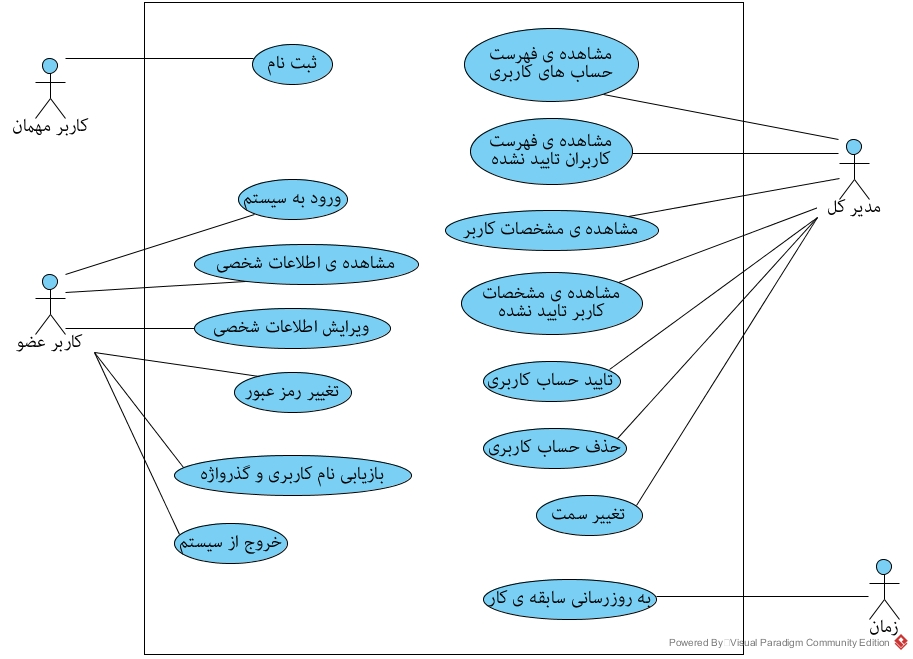
\includegraphics[width=\textwidth]{Diagrams/Accounting.jpg}
\end{center}

\newpage


\begin{tabular}{|p{2cm}|p{10cm}|}
\hline
نام
&
ثبت نام
\\
\hline
شناسه
&
1
\\
\hline
توصیف کوتاه
&
کاربر مهمان در سامانه یک حساب کاربری ایجاد می کند.
\\
\hline
اکتور اولیه
&
کاربر مهمان
\\
\hline
اکتور ثانویه
&

\\
\hline
شرایط ابتدایی
&

\\
\hline
سناریوی اصلی
&
1-	کاربر مهمان با انتخاب گزینه ثبت نام این مورد کاربرد را شروع می کند.
\newline
2-	کاربر مشخصات خود شامل نام، نام خانوادگی، کد ملی ، شماره تلفن، تاریخ تولد، مدرک تحصیلی ، وضعیت تاهل ، سابقه کار و... را وارد میکند.
\newline
3-	با انتخاب گزینه ثبت اطلاعات، مشخصات کاربر مهمان برای مدیر ارسال می شود.
\\
\hline
شرایط نهایی
&
سیستم اطلاعات حساب کاربری را برای مدیر ارسال می کند.
\\
\hline
سناریوی جایگزین
&

\\
\hline
\end{tabular}

\vspace{2cm}


\begin{tabular}{|p{2cm}|p{10cm}|}
\hline
نام
&
مشاهده فهرست حساب های کاربری
\\
\hline
شناسه
&
2
\\
\hline
توصیف کوتاه
&
مدیر فهرست حسابهای کاربری را مشاهد می کند.
\\
\hline
اکتور اولیه
&
مدیرکل
\\
\hline
اکتور ثانویه
&

\\
\hline
شرایط ابتدایی
&
مدیر در سیستم وارد شده باشد.
\\
\hline
سناریوی اصلی
&
1-	مدیر با انتخاب گزینه فهرست حسابهای کاربری، این مورد کاربرد را شروع می کند.
\newline
2-	سیستم حسابهای کاربری موجود را به ترتیب زمان ایجاد نمایش می دهد.
\\
\hline
شرایط نهایی
&
فهرست حسابهای کاربری نمایش داده می شود.
\\
\hline
سناریوی جایگزین
&

\\
\hline
\end{tabular}

\vspace{2cm}


\begin{tabular}{|p{2cm}|p{10cm}|}
\hline
نام
&
مشاهده فهرست کاربران تایید نشده
\\
\hline
شناسه
&
3
\\
\hline
توصیف کوتاه
&
مدیر فهرست حسابهای کاربران مهمان را مشاهد می کند.
\\
\hline
اکتور اولیه
&
مدیرکل
\\
\hline
اکتور ثانویه
&

\\
\hline
شرایط ابتدایی
&
مدیر در سیستم وارد شده باشد.
\\
\hline
سناریوی اصلی
&
1-	مدیر با انتخاب گزینه فهرست کاربران مهمان، این مورد کاربرد را شروع می کند.
\newline
2-	سیستم حسابهای کاربران مهمان موجود را به ترتیب زمان ایجاد نمایش می دهد.
\\
\hline
شرایط نهایی
&
فهرست کاربران مهمان نمایش داده می شود.
\\
\hline
سناریوی جایگزین
&

\\
\hline
\end{tabular}

\vspace{2cm}


\begin{tabular}{|p{2cm}|p{10cm}|}
\hline
نام
&
مشاهده مشخصات کاربر
\\
\hline
شناسه
&
4
\\
\hline
توصیف کوتاه
&
مدیر مشخصات کاربر را مشاهده می کند.
\\
\hline
اکتور اولیه
&
مدیرکل
\\
\hline
اکتور ثانویه
&

\\
\hline
شرایط ابتدایی
&
مدیر در سیستم وارد شده باشد.
\\
\hline
سناریوی اصلی
&
1-	مدیرکل با انتخاب کاربر از فهرست کاربران، این مورد کاربرد را شروع می کند.
\newline
2-	سیستم مشخصات کاربر را نمایش می دهد.
\\
\hline
شرایط نهایی
&
مشخصات کاربر نمایش داده می شود.
\\
\hline
سناریوی جایگزین
&

\\
\hline
\end{tabular}

\vspace{2cm}

\begin{tabular}{|p{2cm}|p{10cm}|}
\hline
نام
&
مشاهده مشخصات کاربر تاییدنشده
\\
\hline
شناسه
&
5
\\
\hline
توصیف کوتاه
&
مدیر مشخصات کاربر مهمان را مشاهده می کند.
\\
\hline
اکتور اولیه
&
مدیرکل
\\
\hline
اکتور ثانویه
&

\\
\hline
شرایط ابتدایی
&
مدیر در سیستم وارد شده باشد.
\\
\hline
سناریوی اصلی
&
1-	مدیرکل با انتخاب کاربر مهمان از فهرست کاربران مهمان، این مورد کاربرد را شروع می کند.
\newline
2-	سیستم مشخصات کاربر مهمان را نمایش می دهد.
\\
\hline
شرایط نهایی
&
مشخصات مهمان کاربر نمایش داده می شود.
\\
\hline
سناریوی جایگزین
&

\\
\hline
\end{tabular}

\vspace{2cm}

\begin{tabular}{|p{2cm}|p{10cm}|}
\hline
نام
&
تایید حساب کاربری
\\
\hline
شناسه
&
6
\\
\hline
توصیف کوتاه
&
مدیر کاربر مهمان را به عنوان یک عضو تایید می کند.
\\
\hline
اکتور اولیه
&
مدیرکل
\\
\hline
اکتور ثانویه
&

\\
\hline
شرایط ابتدایی
&
مدیر در سیستم وارد شده باشد.
\\
\hline
سناریوی اصلی
&
1-	مدیرکل با انتخاب گزینه تایید مهمان، این مورد کاربرد را شروع می کند.
\newline
2-	سیستم مشخصه عضویت کاربر را از مهمان به عضو تغییر می دهد.
\\
\hline
شرایط نهایی
&
مشخصه عضویت کاربر از مهمان به عضو تغییر کند.
\\
\hline
سناریوی جایگزین
&

\\
\hline
\end{tabular}

\vspace{2cm}


\begin{tabular}{|p{2cm}|p{10cm}|}
\hline
نام
&
حذف حساب کاربری
\\
\hline
شناسه
&
7
\\
\hline
توصیف کوتاه
&
مدیر حساب کاربری را از سیستم حذف می کند.
\\
\hline
اکتور اولیه
&
مدیر کل
\\
\hline
اکتور ثانویه
&

\\
\hline
شرایط ابتدایی
&
مدیر در سیستم وارد شده باشد.
\\
\hline
سناریوی اصلی
&
1-	مدیرکل با انتخاب گزینه حذف، این مورد کاربرد را شروع می کند.
\newline
2-	سیستم حساب کاربری را حذف می کند.
\\
\hline
شرایط نهایی
&
حذف حساب کاربری از سیستم
\\
\hline
سناریوی جایگزین
&

\\
\hline
\end{tabular}

\vspace{2cm}


\begin{tabular}{|p{2cm}|p{10cm}|}
\hline
نام
&
تغییر سمت
\\
\hline
شناسه
&
8
\\
\hline
توصیف کوتاه
&
مدیر سمت کاربر عضو را تغییر می دهد.
\\
\hline
اکتور اولیه
&
مدیر کل
\\
\hline
اکتور ثانویه
&

\\
\hline
شرایط ابتدایی
&
مدیر در سیستم وارد شده باشد.
\\
\hline
سناریوی اصلی
&
1-	مدیر با انتخاب یک سمت برای کاربر عضو، این مورد کاربرد را شروع می کند.
\newline
2-	سیستم سمت انتخاب شده را برای کاربر عضو ثبت می کند.
\\
\hline
شرایط نهایی
&
سمت کاربر عضو تغییر کند.
\\
\hline
سناریوی جایگزین
&

\\
\hline
\end{tabular}

\vspace{2cm}


\begin{tabular}{|p{2cm}|p{10cm}|}
\hline
نام
&
به روز رسانی سابقه‌کار
\\
\hline
شناسه
&
9
\\
\hline
توصیف کوتاه
&
پس از گذشت زمان معین، سابقه کار کاربر عضو به روز می شود.
\\
\hline
اکتور اولیه
&
مدیر کل
\\
\hline
اکتور ثانویه
&

\\
\hline
شرایط ابتدایی
&

\\
\hline
سناریوی اصلی
&
1-	پس از گذشت هر 6 ماه از زمان ساخت حساب کاربری، این مورد کاربرد شروع می شود.
\newline
2-	سیستم اطلاعات مربوط به سابقه کار را به علاوه ی 0.5 می کند.
\\
\hline
شرایط نهایی
&
اطلاعات مربوط به سابقه کار به علاوه 0.5 شود.
\\
\hline
سناریوی جایگزین
&

\\
\hline
\end{tabular}

\vspace{2cm}

\begin{tabular}{|p{2cm}|p{10cm}|}
\hline
نام
&
ورود به سیستم
\\
\hline
شناسه
&
10
\\
\hline
توصیف کوتاه
&
کاربر با وارد کردن نام و کلمه عبور وارد سیستم می شود.
\\
\hline
اکتور اولیه
&
کاربر عضو
\\
\hline
اکتور ثانویه
&

\\
\hline
شرایط ابتدایی
&

\\
\hline
سناریوی اصلی
&
1- کاربر با این انتخاب گزینه ورود به سیستم این مورد کاربرد را شروع می کند
\newline
2- کاربر نام کاربری و رمز عبور خود را وارد می کند.
\newline
3- با انتخاب گزینه ورود، کاربر اقدام به ورود می کند.
\newline
4- سیستم اطلاعات کاربر را بررسی می کند.
\newline
5- اگر نام کاربری و رمز عبور کاربر مطابقت داشتند:
\newline
5.1- کاربر وارد سیستم می شود.
\newline
در غیر اینصورت:
\newline
5.2- پیغام خطا جهت ورود صحیح اطلاعات داده می شود.
\\
\hline
شرایط نهایی
&
ورود کاربر و یا مشاهده پیغام خطا
\\
\hline
سناریوی جایگزین
&

\\
\hline
\end{tabular}

\vspace{2cm}


\begin{tabular}{|p{2cm}|p{10cm}|}
\hline
نام
&
ویرایش اطلاعات شخصی
\\
\hline
شناسه
&
11
\\
\hline
توصیف کوتاه
&
کاربر می تواند اطلاعات شخصی خود را تغییر دهد.
\\
\hline
اکتور اولیه
&
کاربر عضو
\\
\hline
اکتور ثانویه
&

\\
\hline
شرایط ابتدایی
&
کاربر به سیستم وارد شده باشد.
\\
\hline
سناریوی اصلی
&
1- کاربر با انتخاب گزینه ویرایش اطلاعات، مورد کاربرد را شروع می کند.
\newline
2- کاربر یک یا چند مورد از اطلاعات شخصی از جمله: نام، نام خانوادگی، کد ملی، شماره تلفن، تاریخ تولد، مدرک تحصیلی، وضعیت تاهل، سابقه کار و ... را تغییر می دهد.
\newline
3- با انتخاب گزینه ثبت اطلاعات، سیستم مشخصات تغییر کرده کاربر را ثبت می کند. 
\\
\hline
شرایط نهایی
&
ثبت مشخصات تغییر کرده کاربر
\\
\hline
سناریوی جایگزین
&

\\
\hline
\end{tabular}

\vspace{2cm}

\begin{tabular}{|p{2cm}|p{10cm}|}
\hline
نام
&
تغییر رمز عبور
\\
\hline
شناسه
&
12
\\
\hline
توصیف کوتاه
&
کاربر رمز عبور خود در سیستم را تغییر می دهد.
\\
\hline
اکتور اولیه
&
کاربر عضو
\\
\hline
اکتور ثانویه
&

\\
\hline
شرایط ابتدایی
&
کاربر به سیستم وارد شده باشد.
\\
\hline
سناریوی اصلی
&
1- کاربر عضو با انتخاب گزینه تغییر رمز عبور این مورد کاربرد را اجرا می کند.
\newline
2- کاربر رمز عبور قبل و رمز عبور جدید را وارد می کند.
\newline
3- با انتخاب گزینه تایید، کاربر عملیات تغییر رمز عبور را آغاز می کند.
\newline
4- اگر رمز عبور قبل با رمز عبور کاربر یکسان بود:
\newline
4.1- سیستم رمز عبور جدید را جایگزین رمز عبور قبلی می کند.
\newline
در غیر اینصورت:
\newline
4.2- سیستم پیغام خطایی مبنی بر درست نبودن رمز عبور قبلی نمایش می دهد.
\\
\hline
شرایط نهایی
&
جایگزین شدن رمز عبور جدید با رمز عبور قبلی و یا نمایش پیغاغم خطا
\\
\hline
سناریوی جایگزین
&

\\
\hline
\end{tabular}

\vspace{2cm}

\begin{tabular}{|p{2cm}|p{10cm}|}
\hline
نام
&
بازیابی نام کاربری و کلمه عبور
\\
\hline
شناسه
&
13
\\
\hline
توصیف کوتاه
&
در صورتی که کاربر نام کاربری یا رمز عبور خود را فراموش کرده باشد،  می تواند با وارد کردن ایمیل آنها را بازیابی می کند.
\\
\hline
اکتور اولیه
&
کاربر عضو
\\
\hline
اکتور ثانویه
&

\\
\hline
شرایط ابتدایی
&
کاربر به سیستم وارد شده باشد.
\\
\hline
سناریوی اصلی
&
1- کاربر با انتخاب گزینه بازیابی اطلاعات، این مورد کاربرد را شروع می کند.
\newline
2- کاربر آدرس پست الکترونیکی خود را در سیستم وارد می کند.
\newline
3- با انتخاب گزینه بازیابی، کاربر موافقت خود را با ارسال ایمیل بازیابی اعلام می کند.
\newline
4- اگر ایمیل داده شده در سیستم موجود باشد:
\newline
4.1- سیستم پیامی حاوی نام کاربری و کلمه عبور را به ایمیل داده شده ارسال می کند.
\newline
در غیر اینصورت:
\newline
4.2- سیستم پیغام خطایی مبنی بر اشتباه بودن ایمیل وارد شده نمایش می دهد.
\\
\hline
شرایط نهایی
&
ارسال ایمیل حاوی نام کاربری و کلمه عبور و یا نمایش پیغام خطا
\\
\hline
سناریوی جایگزین
&

\\
\hline
\end{tabular}

\vspace{2cm}

\begin{tabular}{|p{2cm}|p{10cm}|}
\hline
نام
&
خروج از سیستم
\\
\hline
شناسه
&
14
\\
\hline
توصیف کوتاه
&
کاربر از سیستم خارج می شود.
\\
\hline
اکتور اولیه
&
کاربر عضو
\\
\hline
اکتور ثانویه
&

\\
\hline
شرایط ابتدایی
&
کاربر وارد سیستم شده باشد.
\\
\hline
سناریوی اصلی
&
1- کاربر با انتخاب گزینه خروج، این مورد کاربرد را شروع می کند.
\newline
2- سیستم کاربر را از سیستم خارج می کند.
\\
\hline
شرایط نهایی
&
خروج کاربر از سیستم
\\
\hline
سناریوی جایگزین
&

\\
\hline
\end{tabular}

\vspace{2cm}

\begin{tabular}{|p{2cm}|p{10cm}|}
\hline
نام
&
مشاهده اطلاعات شخصی
\\
\hline
شناسه
&
15
\\
\hline
توصیف کوتاه
&
کاربر اطلاعات شخصی خود را در سیستم مشاهده می کند.
\\
\hline
اکتور اولیه
&
کاربر عضو
\\
\hline
اکتور ثانویه
&

\\
\hline
شرایط ابتدایی
&
کاربر وارد سیستم شده باشد.
\\
\hline
سناریوی اصلی
&
1- کاربر با انتخاب گزینه ی مشاهده پروفایل، این مورد کاربرد را شروع میکند.
\newline
2- سیستم مشخصات کاربر شامل نام، نام خانوادگی، کد ملی ، شماره تلفن، تاریخ تولد، مدرک تحصیلی ، وضعیت تاهل ، سابقه کار و... را نمایش می دهد. 
\\
\hline
شرایط نهایی
&
نمایش مشخصات کاربر
\\
\hline
سناریوی جایگزین
&

\\
\hline
\end{tabular}


\newpage
\subsection{زیرسیستم تولید و نگهداری}

\vspace{2cm}
\begin{center}
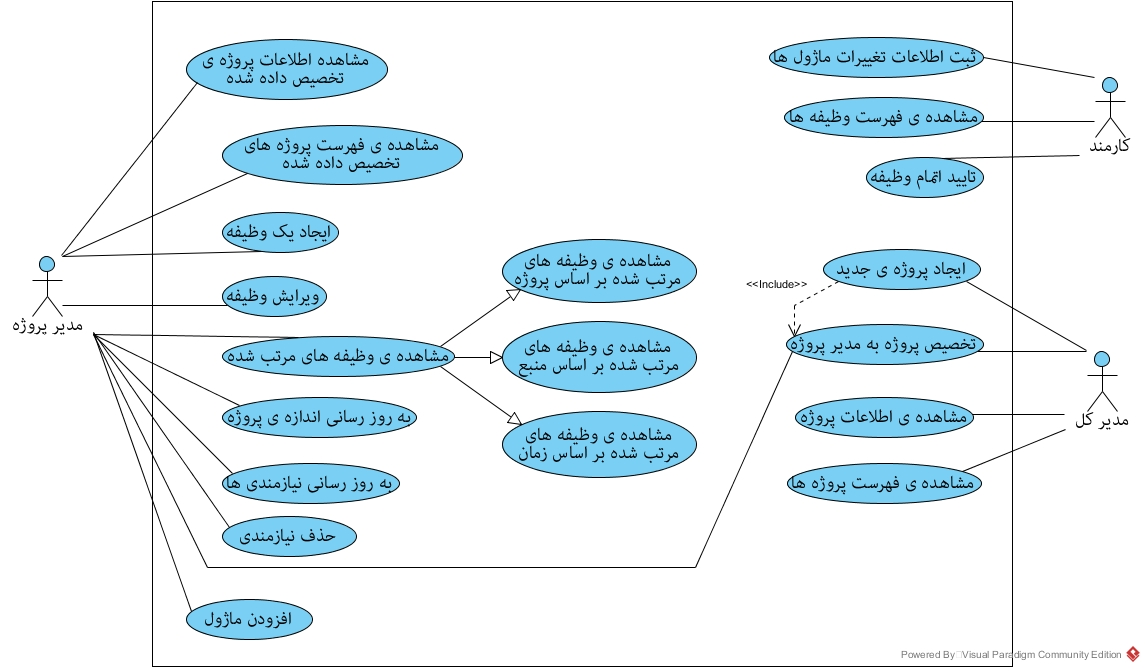
\includegraphics[width=\textwidth]{Diagrams/Development.jpg}
\end{center}

\newpage

\begin{tabular}{|p{2cm}|p{10cm}|}
\hline
نام
&
مشاهده  لیست پروژه های تخصیص داده شده
\\
\hline
شناسه
&
16
\\
\hline
توصیف کوتاه
&
لیستی از پروژه های تخصیص داده شده به یک مدیر پروژه، نمایش داده می شود.
\\
\hline
اکتور اولیه
&
مدیر پروژه
\\
\hline
اکتور ثانویه
&

\\
\hline
شرایط ابتدایی
&
مدیر پروژه وارد حساب کاربری خود شده باشد. 
\\
\hline
سناریوی اصلی
&
1-مدیر پروژه ، با انتخاب مشاهده  لیست پروژه های تخصیص داده شده  این مورد کاربرد را شروع می کند.
\newline
2-سیستم لیست پروژه های تخصیص داده شده به مدیر پروژه را نمایش می دهد
\\
\hline
شرایط نهایی
&
لیست پروژه های تخصیص داده شده به مدیر پروژه نمایش داده می شوند.
\\
\hline
سناریوی جایگزین
&

\\
\hline
\end{tabular}

\vspace{2cm}

\begin{tabular}{|p{2cm}|p{10cm}|}
\hline
نام
&
مشاهده اطلاعات پروژه تخصیص داده شده
\\
\hline
شناسه
&
17
\\
\hline
توصیف کوتاه
&
اطلاعات یک پروژه  تخصیص داده شده به مدیر پروژه نمایش داده می شود.
\\
\hline
اکتور اولیه
&
مدیر پروژه
\\
\hline
اکتور ثانویه
&

\\
\hline
شرایط ابتدایی
&
مدیر پروژه وارد حساب کاربری خود شده باشد
\\
\hline
سناریوی اصلی
&
1-مدیر پروژه ، با انتخاب مشاهده اطلاعات پروژه  تخصیص داده شده این مورد کاربرد را شروع می کند.
\newline
2-سیستم اطلاعات پروژه ی تخصیص داده شده انتخاب شده  توسط مدیر پروژه را نمایش می دهد

\\
\hline
شرایط نهایی
&
مدیر پروژه، اطلاعات پروژه ی تخصیص داده شده انتخاب شده  خود را مشاهده میکند.
\\
\hline
سناریوی جایگزین
&

\\
\hline
\end{tabular}

\vspace{2cm}

\begin{tabular}{|p{2cm}|p{10cm}|}
\hline
نام
&
ایجاد یک وظیفه
\\
\hline
شناسه
&
18
\\
\hline
توصیف کوتاه
&
مدیر پروژه براساس نیازمندی ها، یک وظیفه آماده تخصیص به کارمندان ایجاد میکند.
\\
\hline
اکتور اولیه
&
مدیر پروژه
\\
\hline
اکتور ثانویه
&

\\
\hline
شرایط ابتدایی
&
مدیر پروژه وارد حساب کاربری خود شده باشد. 
\\
\hline
سناریوی اصلی
&
1-مدیر پروژه ، با انتخاب ایجاد یک وظیفه  این مورد کاربرد را شروع می کند.
\newline
2- مدیر پروژه مشخصات وظیفه شامل : عنوان، زمان مورد نیاز و زمان پایان ، ماژول های درگیر و توضیحات لازم را وارد می کند. 
\newline
3-با انتخاب گزینه تایید توسط مدیر پروژه ، وظیفه ایجاد می شود.
\\
\hline
شرایط نهایی
&
ایجاد یک وظیفه
\\
\hline
سناریوی جایگزین
&

\\
\hline
\end{tabular}

\vspace{2cm}

\begin{tabular}{|p{2cm}|p{10cm}|}
\hline
نام
&
ویرایش وظیفه
\\
\hline
شناسه
&
19
\\
\hline
توصیف کوتاه
&
مدیر پروژه اطلاعات یک وظیفه ایجاد شده را ویرایش می کند. 
\\
\hline
اکتور اولیه
&
مدیر پروژه
\\
\hline
اکتور ثانویه
&

\\
\hline
شرایط ابتدایی
&
مدیر پروژه وارد حساب کاربری خود شده باشد. 
\\
\hline
سناریوی اصلی
&
1-مدیر پروژه ، با انتخاب ویرایش وظیفه  این مورد کاربرد را شروع می کند.
\newline
2- مدیر پروژه یک یا چند مورد از مشخصات وظیفه شامل : زمان مورد نیاز و زمان پایان ،وضعیت اتمام،کارمندان انجام دهنده،  ماژول های درگیر و توضیحات لازم را ویراش می کند. 
\newline
3-با انتخاب گزینه تایید توسط مدیر پروژه ، تغییرات دخیره می شوند.
\\
\hline
شرایط نهایی
&
تغییرات وظیفه دخیره می شوند.
\\
\hline
سناریوی جایگزین
&

\\
\hline
\end{tabular}

\vspace{2cm}

\begin{tabular}{|p{2cm}|p{10cm}|}
\hline
نام
&
مشاهده وظیفه های مرتب شده
\\
\hline
شناسه
&
20
\\
\hline
توصیف کوتاه
&
لیست مرتب شده وظیفه ها بر اساس معیار مورد نظر مدیر پروژه ، نمایش داده می شود.
\\
\hline
اکتور اولیه
&
مدیر پروژه
\\
\hline
اکتور ثانویه
&

\\
\hline
شرایط ابتدایی
&
مدیر پروژه وارد حساب کاربری خود شده باشد. 
\\
\hline
سناریوی اصلی
&
1-مدیر پروژه ، با انتخاب مشاهده وظیفه های مرتب شده، این مورد کاربرد را شروع می کند.
\newline
2- مدیر پروژه معیار مورد نظر خود برای مرتب سازی وظیفه ها را انتخاب می کند. 
\newline
3-سیستم لیست مرتب شده وظیفه ها را به مدیر پروژه نمایش می دهد.
\\
\hline
شرایط نهایی
&
لیست مرتب شده وظیفه ها به مدیر پروژه نمایش داده می شود.
\\
\hline
سناریوی جایگزین
&

\\
\hline
\end{tabular}

\vspace{2cm}

\begin{tabular}{|p{2cm}|p{10cm}|}
\hline
نام
&
مشاهده وظیفه های مرتب شده بر اساس پروژه
\\
\hline
شناسه
&
21
\\
\hline
شناسه پدر
&
20
\\
\hline
توصیف کوتاه  
&
لیست مرتب شده وظیفه ها بر اساس پروژه، نمایش داده می شود.
\\
\hline
اکتور اولیه
&
مدیر پروژه
\\
\hline
اکتور ثانویه
&

\\
\hline
شرایط ابتدایی
&
مدیر پروژه وارد حساب کاربری خود شده باشد. 
\\
\hline
سناریوی اصلی
&
1-مدیر پروژه ، با انتخاب مشاهده وظیفه های مرتب شده بر اساس پروژه، این مورد کاربرد را شروع می کند.
\newline
2-سیستم لیست مرتب شده وظیفه های هر پروژه  را به مدیر پروژه نمایش می دهد.
\\
\hline
شرایط نهایی
&
لیست مرتب شده وظیفه های هر پروژه به مدیر پروژه نمایش داده می شود.
\\
\hline
سناریوی جایگزین
&

\\
\hline
\end{tabular}

\vspace{2cm}

\begin{tabular}{|p{2cm}|p{10cm}|}
\hline
نام
&
مشاهده وظیفه های مرتب شده بر اساس منبع
\\
\hline
شناسه
&
22
\\
\hline
شناسه پدر
&
20
\\
\hline
توصیف کوتاه  
&
لیست مرتب شده وظیفه ها بر اساس منبع، نمایش داده می شود.
\\
\hline
اکتور اولیه
&
مدیر پروژه
\\
\hline
اکتور ثانویه
&

\\
\hline
شرایط ابتدایی
&
مدیر پروژه وارد حساب کاربری خود شده باشد. 
\\
\hline
سناریوی اصلی
&
1-مدیر پروژه ، با انتخاب مشاهده وظیفه های مرتب شده بر اساس منبع، این مورد کاربرد را شروع می کند.
\newline
2-سیستم لیست مرتب شده وظیفه های مربوط به هر منبع را به مدیر پروژه نمایش می دهد.
\\
\hline
شرایط نهایی
&
لیست مرتب شده وظیفه های مربوط به هر منبع به مدیر پروژه نمایش داده می شود.
\\
\hline
سناریوی جایگزین
&

\\
\hline
\end{tabular}

\vspace{2cm}

\begin{tabular}{|p{2cm}|p{10cm}|}
\hline
نام
&
مشاهده وظیفه های مرتب شده بر اساس زمان\\
\hline
شناسه
&
23
\\
\hline
شناسه پدر
&
20
\\
\hline
توصیف کوتاه  
&
لیست مرتب شده وظیفه ها بر اساس زمان، نمایش داده می شود.
\\
\hline
اکتور اولیه
&
مدیر پروژه
\\
\hline
اکتور ثانویه
&

\\
\hline
شرایط ابتدایی
&
مدیر پروژه وارد حساب کاربری خود شده باشد. 
\\
\hline
سناریوی اصلی
&
1-مدیر پروژه ، با انتخاب مشاهده وظیفه های مرتب شده بر اساس زمان، این مورد کاربرد را شروع می کند.
\newline
2-سیستم لیست مرتب شده وظیفه ها به ترتیب زمان پایان  آن ها  را به مدیر پروژه نمایش می دهد.
\\
\hline
شرایط نهایی
&
لیست مرتب شده وظیفه ها به ترتیب زمان پایان به مدیر پروژه نمایش داده می شود.
\\
\hline
سناریوی جایگزین
&

\\
\hline
\end{tabular}

\vspace{2cm}

\begin{tabular}{|p{2cm}|p{10cm}|}
\hline
نام
&
به روز رسانی نیازمندی ها
\\
\hline
شناسه
&
24
\\
\hline
توصیف کوتاه
&
مدیر پروژه منابع مورد نیاز پروژه را به روز می کند. 
\\
\hline
اکتور اولیه
&
مدیر پروژه
\\
\hline
اکتور ثانویه
&

\\
\hline
شرایط ابتدایی
&
مدیر پروژه در سیستم وارد شده باشد.
\\
\hline
سناریوی اصلی
&
1-مدیر پروژه با انتخاب گزینه به روزرسانی منابع، این مورد کاربرد را شروع می کند.
\newline
2-سیستم اطلاعات نیازمندی های قبلی پروژه را بازیابی می کند
\newline
3-سیستم فهرست نیازمندی های بازیابی شده را نمایش می دهد
\newline
4-سیستم فیلدهای مربوط به نیازمندی جدید را نمایش می دهد
\newline
5-کاربر فیلدهای داده شده را تکمیل می کند
\newline
6-با انتخاب گزینه افزودن تایید خود را مبنی بر اضافه شدن نیازمندی نشان می دهد
\\
\hline
شرایط نهایی
&
نیازمندی به روز رسانی می‌شود.
\\
\hline
سناریوی جایگزین
&

\\
\hline
\end{tabular}

\vspace{2cm}

\begin{tabular}{|p{2cm}|p{10cm}|}
\hline
نام
&
حذف نیازمندی
\\
\hline
شناسه
&
25
\\
\hline
توصیف کوتاه
&
مدیر پروژه منابع مورد نیاز پروژه را به روز می کند. 
\\
\hline
اکتور اولیه
&
مدیر پروژه
\\
\hline
اکتور ثانویه
&

\\
\hline
شرایط ابتدایی
&
مدیر پروژه در سیستم وارد شده باشد.
\\
\hline
سناریوی اصلی
&
1-مدیر پروژه با انتخاب گزینه حذف نیازمندی، این مورد کاربرد را شروع می کند.
\newline
2-سیستم اطلاعات نیازمندی را از لیست نیازمندی های قبلی پروژه حذف می کند
\\
\hline
شرایط نهایی
&
حذف نیازمندی از نیازمندی های پروژه
\\
\hline
سناریوی جایگزین
&

\\
\hline
\end{tabular}

\vspace{2cm}

\begin{tabular}{|p{2cm}|p{10cm}|}
\hline
نام
&
به روز رسانی اندازه پروژه
\\
\hline
شناسه
&
26
\\
\hline
توصیف کوتاه
&
مدیر پروژه اندازه پروژه را به روز می کند. 
\\
\hline
اکتور اولیه
&
مدیر پروژه
\\
\hline
اکتور ثانویه
&

\\
\hline
شرایط ابتدایی
&
مدیر پروژه در سیستم وارد شده باشد.
\\
\hline
سناریوی اصلی
&
1-مدیر پروژه با انتخاب گزینه به روزرسانی اندازه پروژه، این مورد کاربرد را شروع می کند.
\newline
2-سیستم اطلاعات اندازه فعلی پروژه را بازیابی می کند
\newline
3-سیستم اطلاعات اندازه فعلی پروژه را نمایش می دهد
\newline
4-سیستم فیلدهای مربوط به  تغییرات جدید اندازه را نمایش می دهد
\newline
5-کاربر فیلدهای داده شده را تکمیل می کند
\newline
6-با انتخاب گزینه افزودن تایید خود را مبنی بر اضافه شدن بخش مورد نظر نشان می دهد
\\
\hline
شرایط نهایی
&
اضافه شدن یک بخش مربوط به اندازه پروژه در سیستم
\\
\hline
سناریوی جایگزین
&

\\
\hline
\end{tabular}


\vspace{2cm}


\begin{tabular}{|p{2cm}|p{10cm}|}
\hline
نام
&
ایجاد ماژول
\\
\hline
شناسه
&
27
\\
\hline
توصیف کوتاه
&
مدیر پروژه یک ماژول جدید ایجاد می کند. 
\\
\hline
اکتور اولیه
&
مدیر پروژه
\\
\hline
اکتور ثانویه
&

\\
\hline
شرایط ابتدایی
&
مدیر پروژه در سیستم وارد شده باشد.
\\
\hline
سناریوی اصلی
&
1-مدیر پروژه با انتخاب گزینه ایجاد ماژول، این مورد کاربرد را شروع می کند.
\newline
2-سیستم فیلدهای مربوط به ماژول جدید(شامل: نام، هدف، پروژه مربوط، تسک مربوط و ... ) را نمایش می دهد
\newline
3-کاربر فیلدهای داده شده را تکمیل می کند
\newline
4-با انتخاب گزینه افزودن تایید خود را مبنی بر اضافه شدن ماژول نشان می دهد
\newline
5-ماژول جدید در سیستم ثبت می شود.
\\
\hline
شرایط نهایی
&
اضافه شدن ماژول
\\
\hline
سناریوی جایگزین
&

\\
\hline
\end{tabular}

\vspace{2cm}

\begin{tabular}{|p{2cm}|p{10cm}|}
\hline
نام
&
ثبت اطلاعات تغییر ماژول ها
\\
\hline
شناسه
&
28
\\
\hline
توصیف کوتاه  
&
تغییرات ماژول ها و اطلاعات مربوط به این تغییرات ثبت و نگهداری می شوند.
\\
\hline
اکتور اولیه
&
کارمند
\\
\hline
اکتور ثانویه
&

\\
\hline
شرایط ابتدایی
&
 کارمند وارد حساب کاربری خود شده باشد. 
 \newline
 کاربر به ماژول دسترسی داشته باشد

\\
\hline
سناریوی اصلی
&
1-کارمند، با انتخاب ثبت اطلاعات تغییر ماژول ها، این مورد کاربرد را شروع می کند.
\newline
2-کارمند اطلاعات مربوط به تغییر شامل: فرد/افراد تغییر دهنده،نوع تغییر ، میزان زمان تغییر و منابع مورد استفاده در تغییر را وارد می کند.
\newline
3-با انتخاب گزینه تایید، اطلاعات مربوط به تغییرات ذخیره می شود.
\\
\hline
شرایط نهایی
&
اطلاعات مربوط به تغییرات ماژول ثبت شود.
\\
\hline
سناریوی جایگزین
&

\\
\hline
\end{tabular}

\vspace{2cm}

\begin{tabular}{|p{2cm}|p{10cm}|}
\hline
نام
&
مشاهده لیست وظیفه ها
\\
\hline
شناسه
&
29
\\
\hline
توصیف کوتاه  
&
کارمندان لیست وظیفه های محوله به آن ها را مشاهده می کنند.
\\
\hline
اکتور اولیه
&
کارمند
\\
\hline
اکتور ثانویه
&

\\
\hline
شرایط ابتدایی
&
 کارمند وارد حساب کاربری خود شده باشد. 
\\
\hline
سناریوی اصلی
&
1-کارمند، با انتخاب مشاهده لیست وظیفه ها، این مورد کاربرد را شروع می کند.
\newline
2-سیستم وظیفه های تخصیص داده شده به کارمند را نمایش می دهد.
\\
\hline
شرایط نهایی
&
نمایش وظیفه های تخصیص داده شده به کارمند
\\
\hline
سناریوی جایگزین
&

\\
\hline
\end{tabular}

\vspace{2cm}

\begin{tabular}{|p{2cm}|p{10cm}|}
\hline
نام
&
تایید اتمام وظیفه
\\
\hline
شناسه
&
30
\\
\hline
توصیف کوتاه  
&
کارمند اعلام میکند که وظیفه محول شده به او به پایان رسیده است.
\\
\hline
اکتور اولیه
&
کارمند
\\
\hline
اکتور ثانویه
&

\\
\hline
شرایط ابتدایی
&
 کارمند وارد حساب کاربری خود شده باشد. 
\\
\hline
سناریوی اصلی
&
1-کارمند، با انتخاب تایید اتمام وظیفه، این مورد کاربرد را شروع می کند.
\newline
2-کارمند اتمام انچام وظیفه را در سیستم ثبت می کند.
\\
\hline
شرایط نهایی
&
اتمام وظیفه محول شده به کارمند ثبت می شود.
\\
\hline
سناریوی جایگزین
&

\\
\hline
\end{tabular}

\vspace{2cm}

\begin{tabular}{|p{2cm}|p{10cm}|}
\hline
نام
&
مشاهده  اطلاعات پروژه
\\
\hline
شناسه
&
31
\\
\hline
توصیف کوتاه
&
اطلاعات پروژه به منظور تخصیص منابع به آن، توسط مدیر کل مشاهده می شود.
\\
\hline
اکتور اولیه
&
مدیر کل
\\
\hline
اکتور ثانویه
&

\\
\hline
شرایط ابتدایی
&
مدیر کل وارد سیستم شده باشد. 
\\
\hline
سناریوی اصلی
&
1-مدیر کل ، با انتخاب مشاهده  اطلاعات پروژه، این مورد کاربرد را شروع می کند.
\newline
2-مدیر کل، پروژه مورد نظر خود را انتخاب میکند.
\newline
3-سیستم اطلاعات پروژه را برای مدیر کل نمایش می دهد
\\
\hline
شرایط نهایی
&
اطلاعات پروژه  انتخاب شده توسط مدیر کل مشاهده می شود.
\\
\hline
سناریوی جایگزین
&

\\
\hline
\end{tabular}

\vspace{2cm}

\begin{tabular}{|p{2cm}|p{10cm}|}
\hline
نام
&
 مشاهده  فهرست پروژه ها
\\
\hline
شناسه
&
32
\\
\hline
توصیف کوتاه
&
لیست پروژه ها توسط مدیر کل مشاهده می شود.
\\
\hline
اکتور اولیه
&
مدیر کل
\\
\hline
اکتور ثانویه
&

\\
\hline
شرایط ابتدایی
&
مدیر کل وارد سیستم شده باشد. 
\\
\hline
سناریوی اصلی
&
1-مدیر کل ، با انتخاب مشاهده  فهرست پروژه ها، این مورد کاربرد را شروع می کند.
\newline
2-سیستم فهرست پروژه ها را برای مدیر کل نمایش می دهد
\\
\hline
شرایط نهایی
&
 فهرست پروژه ها توسط مدیر کل مشاهده می شود.
\\
\hline
سناریوی جایگزین
&

\\
\hline
\end{tabular}

\vspace{2cm}


\begin{tabular}{|p{2cm}|p{10cm}|}
\hline
نام
&
ایجاد پروژه ی جدید
\\
\hline
شناسه
&
33
\\
\hline
توصیف کوتاه
&
مدیر کل یک پروژه جدید ایجاد می کند
\\
\hline
اکتور اولیه
&
مدیر کل
\\
\hline
اکتور ثانویه
&

\\
\hline
شرایط ابتدایی
&
مدیر در سیستم وارد شده باشد.
\\
\hline
سناریوی اصلی
&
1-مدیر با انتخاب گزینه ایجاد پروژه جدید، این مورد کاربرد را شروع می کند.
\newline
2-مدیر اطلاعات اولیه پروژه شامل عنوان و توضیحات مربوط به پروژه را وارد می کند.
\newline
3-شامل "تخصیص پروژه به مدیر پروژه"
\newline
3-سیستم پروژه ای جدید با این مشخصات ایجاد می کند. 
\\
\hline
شرایط نهایی
&
ایجاد پروژه جدید
\\
\hline
سناریوی جایگزین
&

\\
\hline
\end{tabular}

\vspace{2cm}

\begin{tabular}{|p{2cm}|p{10cm}|}
\hline
نام
&
تخصیص پروژه به مدیر پروژه
\\
\hline
شناسه
&
34
\\
\hline
توصیف کوتاه
&
مدیر کل یک پروژه را به یک مدیر پروژه تخصیص می دهد
\\
\hline
اکتور اولیه
&
مدیر کل
\\
\hline
اکتور ثانویه
&
مدیر پروژه
\\
\hline
شرایط ابتدایی
&
مدیر در سیستم وارد شده باشد.
\\
\hline
سناریوی اصلی
&
1-مدیر با انتخاب گزینه تخصیص، این مورد کاربرد را شروع می کند.
\newline
2-مدیر از فهرست پروژه های بدون مدیرپروژه یک مورد را انتخاب میکند.
\newline
3-مدیر از فهرست مدیرپروژه های سازمان یک مورد را انتخاب می کند.
\newline
4-با انتخاب گزینه تایید، مدیر، انجام پروژه توسط مدیرپروژه را تایید میکند. 
\newline
5-سیستم اطلاعات مربوط به پروژه و مدیرپروژه را به روزرسانی کرده و پروژه را به مدیر پروژه تخصیص می دهد.
\\
\hline
شرایط نهایی
&
یک پروژه به یک مدیر پروژه تخصیص پیدا کند.
\\
\hline
سناریوی جایگزین
&

\\
\hline
\end{tabular}



\newpage
\subsection{زیرسیستم توزیع}

\vspace{2cm}
\begin{center}
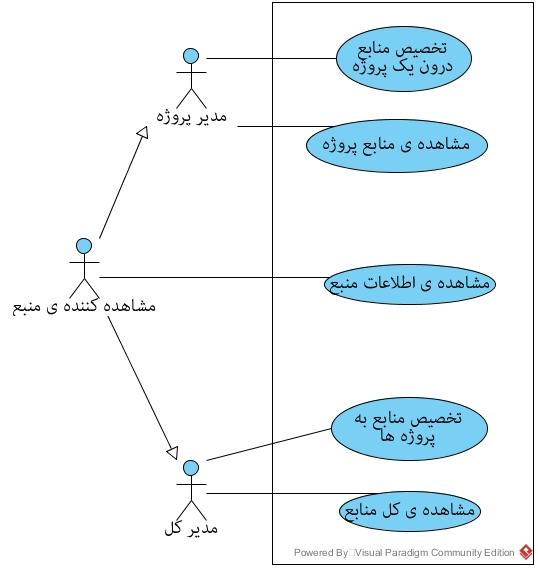
\includegraphics[width=0.7\textwidth]{Diagrams/Resources.jpg}
\end{center}

\newpage

\begin{tabular}{|p{2cm}|p{10cm}|}
\hline
نام
&
مشاهده کل منابع
\\
\hline
شناسه
&
35
\\
\hline
توصیف کوتاه
&
مدیر کل فهرستی از منابع موجود در کل سازمان را مشاهده می کند.
\\
\hline
اکتور اولیه
&
مدیر کل
\\
\hline
اکتور ثانویه
&

\\
\hline
شرایط ابتدایی
&
مدیر در سیستم وارد شده باشد.
\\
\hline
سناریوی اصلی
&
1-مدیر با انتخاب گزینه مشاهده کل منابع، این مورد کاربرد را شروع می کند.
\newline
2-سیستم فهرستی شامل تمامی منابع موجود در سیستم را نمایش می دهد.
\\
\hline
شرایط نهایی
&
نمایش فهرستی منابع موجود
\\
\hline
سناریوی جایگزین
&

\\
\hline
\end{tabular}

\vspace{2cm}

\begin{tabular}{|p{2cm}|p{10cm}|}
\hline
نام
&
مشاهده اطلاعات منبع
\\
\hline
شناسه
&
36
\\
\hline
توصیف کوتاه
&
مشاهده کننده منبع، اطلاعات مربوط به هر منبع و مشغله آن در بازه های زمانی متفاوت را نشان میدهد.
\\
\hline
اکتور اولیه
&
مشاهده کننده ی منبع
\\
\hline
اکتور ثانویه
&

\\
\hline
شرایط ابتدایی
&
مشاهده کننده منبع وارد سیستم شده باشد.
\\
\hline
سناریوی اصلی
&
1-مشاهده کننده منبع با انتخاب گزینه اطلاعات منبع، این مورد کاربرد را شروع می کند.
\newline
2- سیستم تمام پروژه هایی که شامل این منبع بوده اند را برمیگرداند.
\newline
3- پروژه های برگردانده شده به صورت مرتب بر اساس زمان به کاربر نشان داده می شوند.
\\
\hline
شرایط نهایی
&
نمایش مرتب شده پروژه های شامل منبع
\\
\hline
سناریوی جایگزین
&

\\
\hline
\end{tabular}

\vspace{2cm}

\begin{tabular}{|p{2cm}|p{10cm}|}
\hline
نام
&
ویرایش نحوه تخصیص منبع
\\
\hline
شناسه
&
37
\\
\hline
توصیف کوتاه
&
مدیرکل می تواند نحوه تخصیص منبع مورد نظر را ویرایش کند. 
\\
\hline
اکتور اولیه
&
مدیر کل
\\
\hline
اکتور ثانویه
&

\\
\hline
شرایط ابتدایی
&
مدیر کل وارد سیستم شده باشد.
\\
\hline
سناریوی اصلی
&
1-مدیر کل گزینه ویرایش نحوه تخصیص منبع را انتخاب می کند.
\newline
2-مدیر با انتخاب هریک از بازه های زمانی پروژه ای را تغییر داده یا اضافه و یا حذف می کند.
\newline
3- مدیرکل با انتخاب گزینه تایید ویرایش، موافقت خود با ثبت تغییرات را اعلام می کند.
\newline
4- سیستم اطلاعات مربوط به تغییر، حذف یا اضافه شدن منبع به پروژه های مختلف را ذخیره می کند.  
\\
\hline
شرایط نهایی
&
ثبت اطلاعات مربوط به تغییر منابع اختصاص شده به پروژه های مختلف.
\\
\hline
سناریوی جایگزین
&

\\
\hline
\end{tabular}

\vspace{2cm}

\begin{tabular}{|p{2cm}|p{10cm}|}
\hline
نام
&
مشاهده نحوه تخصیص منبع یک پروژه
\\
\hline
شناسه
&
38
\\
\hline
توصیف کوتاه
&
مدیر پروژه فهرستی از منابع موجود در پروژه را مشاهده می کند.
\\
\hline
اکتور اولیه
&
مدیر کل
\\
\hline
اکتور ثانویه
&

\\
\hline
شرایط ابتدایی
&
مدیرپروژه در سیستم وارد شده باشد.
\\
\hline
سناریوی اصلی
&
1-مدیرپروژه با انتخاب گزینه مشاهده منابع، این مورد کاربرد را شروع می کند.
\newline
2-مدیر پروژه پروژه مورد نظر را انتخاب می کند.
\newline
3-مدیر پروژه با انتخاب گزینه تایید، موافقت خود را با پروژه انتخابی نشان می دهد.
\newline
4-سیستم فهرستی شامل منابع مربوط به پروژه انتخاب شده نمایش می دهد.
\\
\hline
شرایط نهایی
&
نمایش فهرستی منابع مربوط به پروژه
\\
\hline
سناریوی جایگزین
&

\\
\hline
\end{tabular}

\vspace{2cm}

\begin{tabular}{|p{2cm}|p{10cm}|}
\hline
نام
&
ویرایش نحوه تخصیص منبع یک پروژه
\\
\hline
شناسه
&
39
\\
\hline
توصیف کوتاه
&
مدیر پروژه می تواند نحوه تخصیص منبع مورد نظر را ویرایش کند. 
\\
\hline
اکتور اولیه
&
مدیر پروژه
\\
\hline
اکتور ثانویه
&

\\
\hline
شرایط ابتدایی
&
مدیر پروژه وارد سیستم شده باشد.
\\
\hline
سناریوی اصلی
&
1-مدیر پروژه گزینه ویرایش نحوه تخصیص منبع را انتخاب می کند.
\newline
2-مدیر با انتخاب هریک از بازه های زمانی ماژولی را تغییر داده یا اضافه و یا حذف می کند.
\newline
3- مدیر پروژه با انتخاب گزینه تایید ویرایش، موافقت خود با ثبت تغییرات را اعلام می کند.
\newline
4- سیستم اطلاعات مربوط به تغییر، حذف یا اضافه شدن منبع به ماژولهای مختلف را ذخیره می کند.  
\\
\hline
شرایط نهایی
&
ثبت اطلاعات مربوط به تغییر منابع اختصاص شده به ماژول‌های مختلف.
\\
\hline
سناریوی جایگزین
&

\\
\hline
\end{tabular}


\newpage
\subsection{زیرسیستم گزارش‌گیری}

\vspace{2cm}
\begin{center}
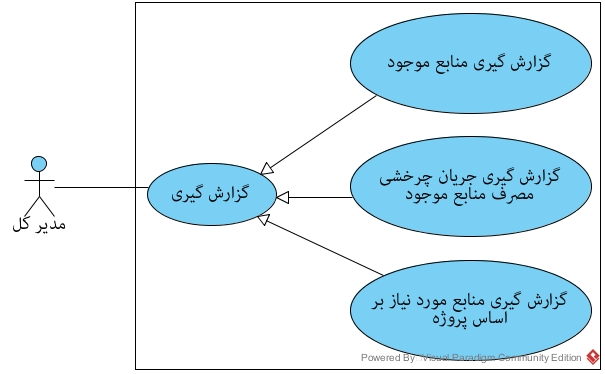
\includegraphics[width=\textwidth]{Diagrams/Reporting.jpg}
\end{center}

\newpage

\begin{tabular}{|p{2cm}|p{10cm}|}
\hline
نام
&
گزارش گیری منابع موجود
\\
\hline
شناسه
&
40
\\
\hline
شناسه پدر
&
43
\\
\hline
توصیف کوتاه
&
گزارشی از اینکه هر منبع به چه میزان و در کدام قسمت موجود است نمایش داده می شود
\\
\hline
اکتور اولیه
&
مدیر کل
\\
\hline
اکتور ثانویه
&

\\
\hline
شرایط ابتدایی
&

\\
\hline
سناریوی اصلی
&
1-مدیر با انتخاب گزارش گیری منابع موجود  این مورد کاربرد را شروع می کند.
\newline
2-مدیر پروژه یا پروژه های مورد نظر خود را مشخص میکند.
\newline
3-با انتخاب گزینه دریافت گزارش ، سیستم منابع موجود در هر قسمت در پروژه/پروژه های مورد نظر را نمایش می دهد. 
\\
\hline
شرایط نهایی
&

\\
\hline
سناریوی جایگزین
&

\\
\hline
\end{tabular}

\vspace{2cm}

\begin{tabular}{|p{2cm}|p{10cm}|}
\hline
نام
&
گزارش گیری جریان چرخشی مصرف منابع موجود
\\
\hline
شناسه
&
41
\\
\hline
شناسه پدر
&
43
\\
\hline
توصیف کوتاه
&
گزارشی حاوی میزان استفاده از منابع تحت عنوان گزارش جریان چرخشی منابع نمایش داده می شود.
\\
\hline
اکتور اولیه
&
مدیر کل
\\
\hline
اکتور ثانویه
&

\\
\hline
شرایط ابتدایی
&

\\
\hline
سناریوی اصلی
&
1-مدیر با انتخاب گزارش گیری جریان چرخشی مصرف منابع موجود این مورد کاربرد را شروع می کند.
\newline
2-مدیر بازه زمانی مورد نظر خود را وارد میکند.
\newline
3-با انتخاب گزینه دریافت گزارش، سیستم میزان استفاده از منابع موجود در هر قسمت در بازه زمانی مورد نظر را نمایش می دهد. 
\\
\hline
شرایط نهایی
&

\\
\hline
سناریوی جایگزین
&

\\
\hline
\end{tabular}

\vspace{2cm}

\begin{tabular}{|p{2cm}|p{10cm}|}
\hline
نام
&
گزارش گیری منابع مورد نیاز براساس پروژه
\\
\hline
شناسه
&
42
\\
\hline
شناسه پدر
&
43
\\
\hline
توصیف کوتاه
&
گزارش حاوی منابع موجود در هر پروژه نمایش داده می شود.
\\
\hline
اکتور اولیه
&
مدیر کل
\\
\hline
اکتور ثانویه
&

\\
\hline
شرایط ابتدایی
&

\\
\hline
سناریوی اصلی
&
1-مدیر با انتخاب گزارش گیری منابع مورد نیاز براساس پروژه این مورد کاربرد را شروع می کند.
\newline
2-مدیر پروژه یا پروژه های مورد نظر خود را مشخص میکند. 
\newline
3-با انتخاب گزینه دریافت گزارش، سیستم  منابع مورد استفاده در پروژه/پروژه های مورد نظر را نمایش می دهد. 

\\
\hline
شرایط نهایی
&

\\
\hline
سناریوی جایگزین
&

\\
\hline
\end{tabular}

\vspace{2cm}

\begin{tabular}{|p{2cm}|p{10cm}|}
\hline
نام
&
گزارش گیری
\\
\hline
شناسه
&
43
\\
\hline
توصیف کوتاه
&
گزارشی از منابع توسط مدیر دریافت می شود.
\\
\hline
اکتور اولیه
&
مدیر کل 
\\
\hline
اکتور ثانویه
&

\\
\hline
شرایط ابتدایی
&
مدیر وارد حساب کاربری خود شده باشد
\\
\hline
سناریوی اصلی
&

\\
\hline
شرایط نهایی
&
گزارش از سیستم گرفته می شود.
\\
\hline
سناریوی جایگزین
&

\\
\hline
\end{tabular}



\newpage
\subsection{زیرسیستم پیش‌بینی}

\vspace{2cm}
\begin{center}
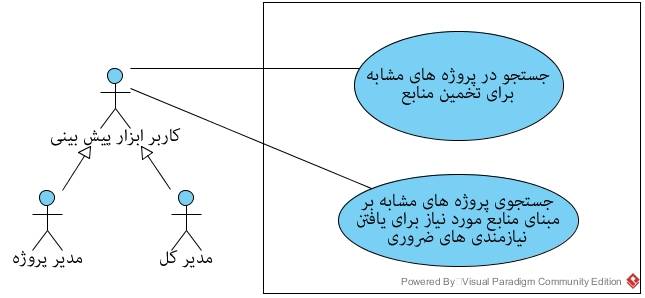
\includegraphics[width=\textwidth]{Diagrams/Anticipating.jpg}
\end{center}


\newpage
\begin{tabular}{|p{2cm}|p{10cm}|}
\hline
نام
&
جستجو در پروژه های مشابه برای تخمین منابع
\\
\hline
شناسه
&
44
\\
\hline
توصیف کوتاه
&
کاربر ابزار پیش‌بینی در میان پروژه‌های موجود بر اساس ویژگی‌های مختلف جستجو می‌کند.
\\
\hline
اکتور اولیه
&
کاربر ابزار پیش‌بینی
\\
\hline
اکتور ثانویه
&

\\
\hline
شرایط ابتدایی
&
کاربر ابزار پیش‌بینی در سیستم وارد شده باشد.
\\
\hline
سناریوی اصلی
&
1- کاربر ابزار پیش‌بینی با انتخاب گزینه‌ی جستجوی پروژه، این مورد کاربرد را شروع می‌کند.
\newline
2- کاربر ابزار پیش‌بینی بازه‌ی سایز و تکنولوژی مورد نظرش را وارد می‌کند.
\newline
3- سیستم فهرستی از پروژه‌ها با ویژگی‌های مورد نظر را نمایش می‌دهد.
\\
\hline
شرایط نهایی
&
فهرستی از پروژه‌ها با ویژگی‌های مورد نظر نمایش داده می‌شود.
\\
\hline
سناریوی جایگزین
&

\\
\hline
\end{tabular}

\vspace{2cm}

\begin{tabular}{|p{2cm}|p{10cm}|}
\hline
نام
&
جستجوی پروژه های مشابه بر مبنای منابع مورد نیاز برای یافتن نیازمندی های ضروری
\\
\hline
شناسه
&
45
\\
\hline
توصیف کوتاه
&
کاربر ابزار پیش‌بینی در میان پروژه‌های موجود بر اساس منابع مورد نیاز، جستجو می‌کند.
\\
\hline
اکتور اولیه
&
کاربر ابزار پیش‌بینی
\\
\hline
اکتور ثانویه
&

\\
\hline
شرایط ابتدایی
&
کاربر ابزار پیش‌بینی در سیستم وارد شده باشد.
\\
\hline
سناریوی اصلی
&
1- کاربر ابزار پیش‌بینی با انتخاب گزینه‌ی جستجو بر اساس منابع، این مورد کاربرد را شروع می‌کند.
\newline
2- کاربر ابزار پیش‌بینی منابع مورد نیاز را وارد می‌کند.
\newline
3- سیستم فهرستی از پروژه‌ها با منابع مشابه و نیازمندی‌های ضروری این پروژه‌ها را نمایش می‌دهد.
\\
\hline
شرایط نهایی
&
فهرستی از پروژه‌ها با منابع مشابه و نیازمندی‌های ضروری آن‌ها نشان داده می‌شود.
\\
\hline
سناریوی جایگزین
&

\\
\hline
\end{tabular}


\newpage
\section{نمودارهای فعالیت}

نکته‌ای در مورد نمودارهای فعالیت:
\\
در همه‌ی فعالیت‌ها امکان انصراف از انجام فعالیت وجود دارد.

\vspace{1cm}
\subsection{زیرسیستم کاربری}

\vspace{1cm}
\subsection*{مورد کاربرد ثبت نام}
\vspace{2cm}
\begin{center}
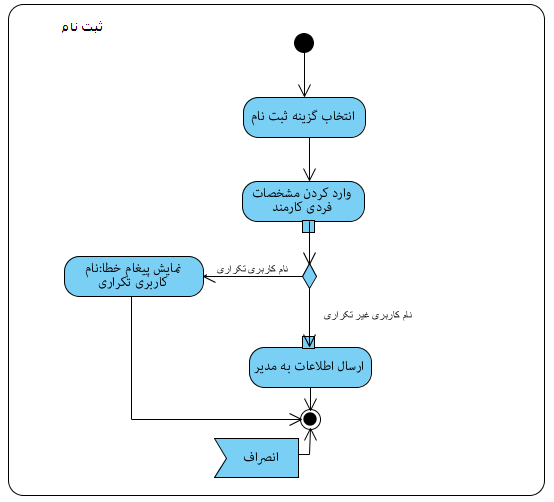
\includegraphics[width=\textwidth]{ActivityDiagrams/1.png}
\end{center}

\newpage
\vspace{2cm}
\subsection*{مورد کاربرد مشاهده فهرست حساب‌های کاربری}
\vspace{2cm}
\begin{center}
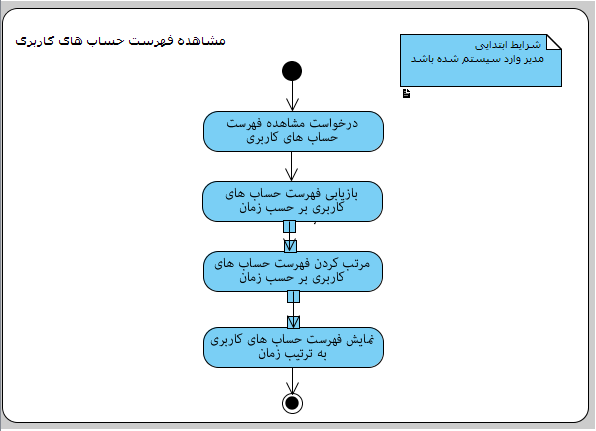
\includegraphics[width=\textwidth]{ActivityDiagrams/2.png}
\end{center}

\newpage
\vspace{2cm}
\subsection*{مورد کاربرد مشاهده فهرست کاربران تایید نشده}
\vspace{2cm}
\begin{center}
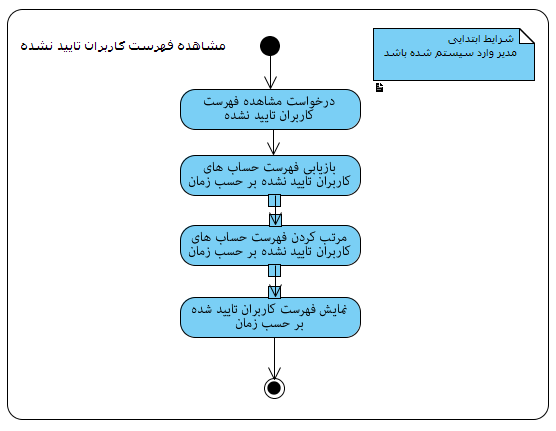
\includegraphics[width=\textwidth]{ActivityDiagrams/3.png}
\end{center}

\newpage
\vspace{2cm}
\subsection*{مورد کاربرد مشاهده مشخصات کاربر}
\vspace{2cm}
\begin{center}
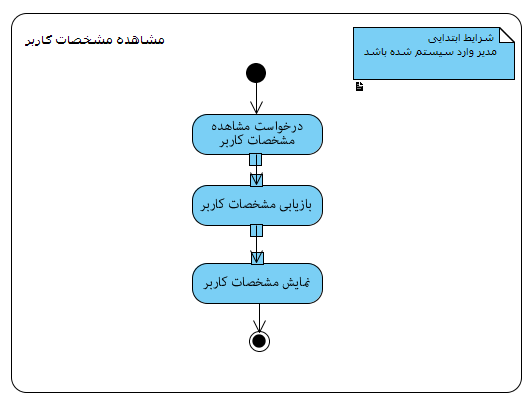
\includegraphics[width=\textwidth]{ActivityDiagrams/4.png}
\end{center}

\newpage
\vspace{2cm}
\subsection*{مورد کاربرد مشخصات کاربر تایید نشده}
\vspace{2cm}
\begin{center}
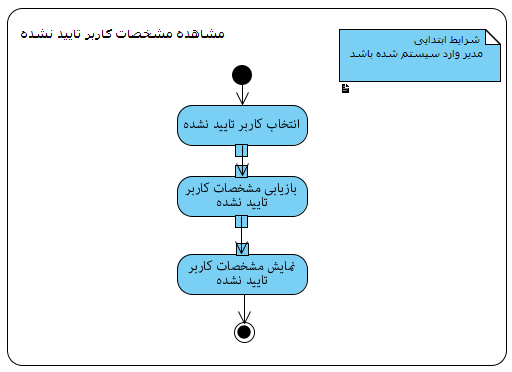
\includegraphics[width=\textwidth]{ActivityDiagrams/5.png}
\end{center}

\newpage
\vspace{2cm}
\subsection*{مورد کاربرد تایید حساب کاربری}
\vspace{2cm}
\begin{center}
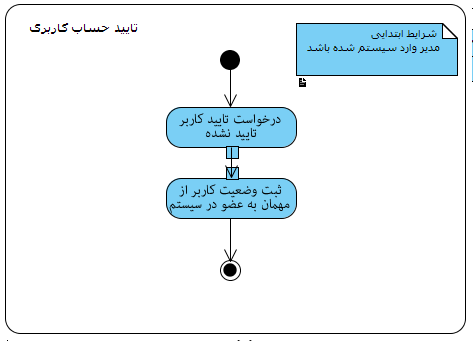
\includegraphics[width=\textwidth]{ActivityDiagrams/6.png}
\end{center}

\newpage
\vspace{2cm}
\subsection*{مورد کاربرد حذف حساب کاربری}
\vspace{2cm}
\begin{center}
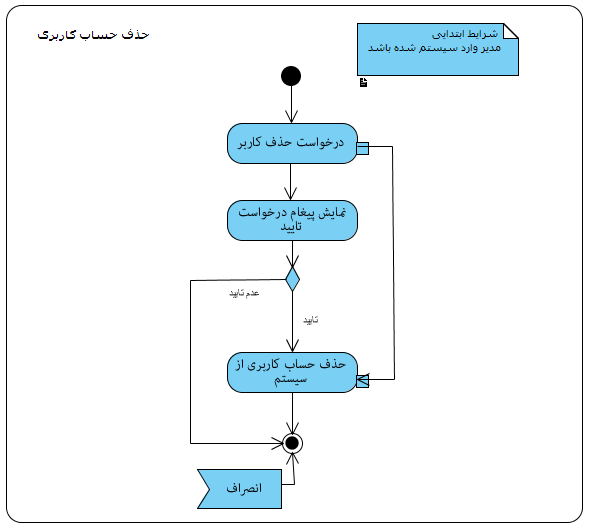
\includegraphics[width=\textwidth]{ActivityDiagrams/7.png}
\end{center}

\newpage
\vspace{2cm}
\subsection*{مورد کاربرد تغییر سمت}
\vspace{2cm}
\begin{center}
\includegraphics[width=\textwidth]{ActivityDiagrams/8.png}
\end{center}

\newpage
\vspace{2cm}
\subsection*{مورد کاربرد به روزرسانی سابقه کار}
\vspace{2cm}
\begin{center}
\includegraphics[width=\textwidth]{ActivityDiagrams/9.png}
\end{center}

\newpage
\vspace{2cm}
\subsection*{مورد کاربرد ورود به سیستم}
\vspace{2cm}
\begin{center}
\includegraphics[width=\textwidth]{ActivityDiagrams/10.png}
\end{center}

\newpage
\vspace{2cm}
\subsection*{مورد کاربرد ویرایش اطلاعات شخصی}
\vspace{2cm}
\begin{center}
\includegraphics[width=\textwidth]{ActivityDiagrams/11.png}
\end{center}

\newpage
\vspace{2cm}
\subsection*{مورد کاربرد تغییر رمز عبور}
\vspace{2cm}
\begin{center}
\includegraphics[width=\textwidth]{ActivityDiagrams/12.png}
\end{center}

\newpage
\vspace{2cm}
\subsection*{مورد کاربرد بازیابی نام کاربری و کلمه عبور}
\vspace{2cm}
\begin{center}
\includegraphics[width=\textwidth]{ActivityDiagrams/13.png}
\end{center}

\newpage
\vspace{2cm}
\subsection*{مورد کاربرد خروج از سیستم}
\vspace{2cm}
\begin{center}
\includegraphics[width=\textwidth]{ActivityDiagrams/14.png}
\end{center}

\newpage
\vspace{2cm}
\subsection*{مورد کاربرد مشاهده اطلاعات شخصی}
\vspace{2cm}
\begin{center}
\includegraphics[width=\textwidth]{ActivityDiagrams/15.png}
\end{center}

\newpage
\subsection{زیرسیستم تولید و نگهداری}

\vspace{2cm}
\subsection*{مورد کاربرد مشاهده لیست پروژه های تخصیص داده شده}
\vspace{2cm}
\begin{center}
\includegraphics[width=\textwidth]{ActivityDiagrams/16.jpg}
\end{center}


\newpage
\vspace{2cm}
\subsection*{مورد کاربرد مشاهده اطلاعات پروژه تخصیص داده شده}
\vspace{2cm}
\begin{center}
\includegraphics[width=\textwidth]{ActivityDiagrams/17.jpg}
\end{center}

\newpage
\vspace{2cm}
\subsection*{مورد کاربرد ایجاد یک وظیفه}
\vspace{2cm}
\begin{center}
\includegraphics[width=\textwidth]{ActivityDiagrams/18.jpg}
\end{center}

\newpage
\vspace{2cm}
\subsection*{مورد کاربرد ویرایش وظیفه}
\vspace{2cm}
\begin{center}
\includegraphics[width=\textwidth]{ActivityDiagrams/19.jpg}
\end{center}

\newpage
\vspace{2cm}
\subsection*{مورد کاربرد مشاهده وظیفه‌های مرتب‌شده}
\vspace{2cm}
\begin{center}
\includegraphics[width=\textwidth]{ActivityDiagrams/20.jpg}
\end{center}

\newpage
\vspace{2cm}
\subsection*{مورد کاربرد به روز رسانی نیازمندی‌ها}
\vspace{2cm}
\begin{center}
\includegraphics[width=\textwidth]{ActivityDiagrams/24.jpg}
\end{center}

\newpage
\vspace{2cm}
\subsection*{مورد کاربرد حذف نیازمندی}
\vspace{2cm}
\begin{center}
\includegraphics[width=\textwidth]{ActivityDiagrams/25.jpg}
\end{center}

\newpage
\vspace{2cm}
\subsection*{مورد کاربرد به روز رسانی اندازه‌ی پروژه}
\vspace{2cm}
\begin{center}
\includegraphics[width=\textwidth]{ActivityDiagrams/26.jpg}
\end{center}

\newpage
\vspace{2cm}
\subsection*{مورد کاربرد ایجاد ماژول}
\vspace{2cm}
\begin{center}
\includegraphics[width=\textwidth]{ActivityDiagrams/27.jpg}
\end{center}


\newpage
\vspace{2cm}
\subsection*{مورد کاربرد ثبت اطلاعات تغییر ماژول‌ها}
\vspace{2cm}
\begin{center}
\includegraphics[width=\textwidth]{ActivityDiagrams/28.jpg}
\end{center}

\newpage
\vspace{2cm}
\subsection*{مورد کاربرد مشاهده لیست وظیفه‌ها}
\vspace{2cm}
\begin{center}
\includegraphics[width=\textwidth]{ActivityDiagrams/29.jpg}
\end{center}

\newpage
\vspace{2cm}
\subsection*{مورد کاربرد تایید اتمام وظیفه}
\vspace{2cm}
\begin{center}
\includegraphics[width=\textwidth]{ActivityDiagrams/30.jpg}
\end{center}

\newpage
\vspace{2cm}
\subsection*{مورد کاربرد مشاهده اطلاعات پروژه}
\vspace{2cm}
\begin{center}
\includegraphics[width=\textwidth]{ActivityDiagrams/31.jpg}
\end{center}
\newpage
\vspace{2cm}
\subsection*{مورد کاربرد مشاهده فهرست پروژه‌ها}
\vspace{2cm}
\begin{center}
\includegraphics[width=\textwidth]{ActivityDiagrams/32.jpg}
\end{center}

\newpage
\vspace{2cm}
\subsection*{مورد کاربرد ایجاد پروژه جدید}
\vspace{2cm}
\begin{center}
\includegraphics[width=\textwidth]{ActivityDiagrams/33.jpg}
\end{center}

\newpage
\vspace{1cm}
\subsection*{مورد کاربرد تخصیص پروژه به مدیر پروژه}
\vspace{1cm}
\begin{center}
\includegraphics[width=0.8\textwidth]{ActivityDiagrams/34.jpg}
\end{center}


\subsection{زیرسیستم توزیع}
\vspace{1cm}
\subsection*{مورد کاربرد مشاهده کل منابع}
\vspace{1cm}
\begin{center}
\includegraphics[width=\textwidth]{ActivityDiagrams/35.jpg}
\end{center}

\newpage
\vspace{1cm}
\subsection*{مورد کاربرد مشاهده اطلاعات منابع}
\vspace{2cm}
\begin{center}
\includegraphics[width=\textwidth]{ActivityDiagrams/36.jpg}
\end{center}

\newpage
\vspace{2cm}
\subsection*{مورد کاربرد ویرایش نحوه تخصیص منبع}
\vspace{2cm}
\begin{center}
\includegraphics[width=\textwidth]{ActivityDiagrams/37.jpg}
\end{center}

\newpage
\vspace{2cm}
\subsection*{مورد کاربرد مشاهده نحوه تخصیص منبع یک پروژه}
\vspace{2cm}
\begin{center}
\includegraphics[width=\textwidth]{ActivityDiagrams/38.jpg}
\end{center}

\newpage
\vspace{2cm}
\subsection*{مورد کاربرد ویرایش نحوه تخصیص منبع یک پروژه}
\vspace{2cm}
\begin{center}
\includegraphics[width=\textwidth]{ActivityDiagrams/39.jpg}
\end{center}



\newpage
\subsection{زیرسیستم گزارش‌گیری}

\vspace{2cm}
\subsection*{مورد کاربرد گزارش‌گیری منابع موجود}
\vspace{2cm}
\begin{center}
\includegraphics[width=\textwidth]{ActivityDiagrams/40.jpg}
\end{center}

\newpage
\vspace{2cm}
\subsection*{مورد کاربرد گزارش‌گیری جریان چرخشی منابع موجود}
\vspace{2cm}
\begin{center}
\includegraphics[width=\textwidth]{ActivityDiagrams/41.jpg}
\end{center}

\newpage
\vspace{2cm}
\subsection*{مورد کاربرد گزارش‌گیری منابع موردنیاز بر اساس پروژه}
\vspace{2cm}
\begin{center}
\includegraphics[width=\textwidth]{ActivityDiagrams/42.jpg}
\end{center}


\newpage
\subsection{زیرسیستم پیش‌بینی}

\vspace{2cm}
\subsection*{مورد کاربرد جستجو در پروژه‌های مشابه برای تخمین منابع}
\vspace{2cm}
\begin{center}
\includegraphics[width=\textwidth]{ActivityDiagrams/44.jpg}
\end{center}

\newpage
\vspace{2cm}
\subsection*{مورد کاربرد جستجوی پروژه‌های مشابه بر مبنای منابع مورد نیاز برای یافتن نیازمندی‌های ضروری}
\vspace{2cm}
\begin{center}
\includegraphics[width=\textwidth]{ActivityDiagrams/45.jpg}
\end{center}


\newpage
\section{نمودارهای فعالیت غنی‌شده}

نکته‌ای در مورد نمودارهای فعالیت:
\\
در همه‌ی فعالیت‌ها امکان انصراف از انجام فعالیت وجود دارد.

\vspace{1cm}
\subsection{زیرسیستم کاربری}

\vspace{1cm}
\subsection*{مورد کاربرد ثبت نام}
\vspace{2cm}
\begin{center}
\includegraphics[width=\textwidth]{ActivityDiagramsWithSwimlanes/1.png}
\end{center}

\newpage
\vspace{2cm}
\subsection*{مورد کاربرد مشاهده فهرست حساب‌های کاربری}
\vspace{2cm}
\begin{center}
\includegraphics[width=\textwidth]{ActivityDiagramsWithSwimlanes/2.png}
\end{center}

\newpage
\vspace{2cm}
\subsection*{مورد کاربرد مشاهده فهرست کاربران تایید نشده}
\vspace{2cm}
\begin{center}
\includegraphics[width=\textwidth]{ActivityDiagramsWithSwimlanes/3.png}
\end{center}

\newpage
\vspace{2cm}
\subsection*{مورد کاربرد مشاهده مشخصات کاربر}
\vspace{2cm}
\begin{center}
\includegraphics[width=\textwidth]{ActivityDiagramsWithSwimlanes/4.png}
\end{center}

\newpage
\vspace{2cm}
\subsection*{مورد کاربرد مشخصات کاربر تایید نشده}
\vspace{2cm}
\begin{center}
\includegraphics[width=\textwidth]{ActivityDiagramsWithSwimlanes/5.png}
\end{center}

\newpage
\vspace{2cm}
\subsection*{مورد کاربرد تایید حساب کاربری}
\vspace{2cm}
\begin{center}
\includegraphics[width=\textwidth]{ActivityDiagramsWithSwimlanes/6.png}
\end{center}

\newpage
\vspace{2cm}
\subsection*{مورد کاربرد حذف حساب کاربری}
\vspace{2cm}
\begin{center}
\includegraphics[width=\textwidth]{ActivityDiagramsWithSwimlanes/7.png}
\end{center}

\newpage
\vspace{2cm}
\subsection*{مورد کاربرد تغییر سمت}
\vspace{2cm}
\begin{center}
\includegraphics[width=\textwidth]{ActivityDiagramsWithSwimlanes/8.png}
\end{center}

\newpage
\vspace{2cm}
\subsection*{مورد کاربرد به روزرسانی سابقه کار}
\vspace{2cm}
\begin{center}
\includegraphics[width=\textwidth]{ActivityDiagramsWithSwimlanes/9.png}
\end{center}

\newpage
\vspace{2cm}
\subsection*{مورد کاربرد ورود به سیستم}
\vspace{2cm}
\begin{center}
\includegraphics[width=\textwidth]{ActivityDiagramsWithSwimlanes/10.png}
\end{center}

\newpage
\vspace{2cm}
\subsection*{مورد کاربرد ویرایش اطلاعات شخصی}
\vspace{2cm}
\begin{center}
\includegraphics[width=\textwidth]{ActivityDiagramsWithSwimlanes/11.png}
\end{center}

\newpage
\vspace{2cm}
\subsection*{مورد کاربرد تغییر رمز عبور}
\vspace{2cm}
\begin{center}
\includegraphics[width=\textwidth]{ActivityDiagramsWithSwimlanes/12.png}
\end{center}

\newpage
\vspace{2cm}
\subsection*{مورد کاربرد بازیابی نام کاربری و کلمه عبور}
\vspace{2cm}
\begin{center}
\includegraphics[width=\textwidth]{ActivityDiagramsWithSwimlanes/13.png}
\end{center}

\newpage
\vspace{2cm}
\subsection*{مورد کاربرد خروج از سیستم}
\vspace{2cm}
\begin{center}
\includegraphics[width=\textwidth]{ActivityDiagramsWithSwimlanes/14.png}
\end{center}

\newpage
\vspace{2cm}
\subsection*{مورد کاربرد مشاهده اطلاعات شخصی}
\vspace{2cm}
\begin{center}
\includegraphics[width=\textwidth]{ActivityDiagramsWithSwimlanes/15.png}
\end{center}

\newpage
\subsection{زیرسیستم تولید و نگهداری}

\vspace{2cm}
\subsection*{مورد کاربرد مشاهده لیست پروژه های تخصیص داده شده}
\vspace{2cm}
\begin{center}
\includegraphics[width=\textwidth]{ActivityDiagramsWithSwimlanes/16.jpg}
\end{center}


\newpage
\vspace{2cm}
\subsection*{مورد کاربرد مشاهده اطلاعات پروژه تخصیص داده شده}
\vspace{2cm}
\begin{center}
\includegraphics[width=\textwidth]{ActivityDiagramsWithSwimlanes/17.jpg}
\end{center}

\newpage
\vspace{2cm}
\subsection*{مورد کاربرد ایجاد یک وظیفه}
\vspace{2cm}
\begin{center}
\includegraphics[width=\textwidth]{ActivityDiagramsWithSwimlanes/18.jpg}
\end{center}

\newpage
\vspace{2cm}
\subsection*{مورد کاربرد ویرایش وظیفه}
\vspace{2cm}
\begin{center}
\includegraphics[width=\textwidth]{ActivityDiagramsWithSwimlanes/19.jpg}
\end{center}

\newpage
\vspace{2cm}
\subsection*{مورد کاربرد مشاهده وظیفه‌های مرتب‌شده}
\vspace{2cm}
\begin{center}
\includegraphics[width=\textwidth]{ActivityDiagramsWithSwimlanes/20.jpg}
\end{center}

\newpage
\vspace{2cm}
\subsection*{مورد کاربرد به روز رسانی نیازمندی‌ها}
\vspace{2cm}
\begin{center}
\includegraphics[width=\textwidth]{ActivityDiagramsWithSwimlanes/24.jpg}
\end{center}

\newpage
\vspace{2cm}
\subsection*{مورد کاربرد حذف نیازمندی}
\vspace{2cm}
\begin{center}
\includegraphics[width=\textwidth]{ActivityDiagramsWithSwimlanes/25.jpg}
\end{center}

\newpage
\vspace{2cm}
\subsection*{مورد کاربرد به روز رسانی اندازه‌ی پروژه}
\vspace{2cm}
\begin{center}
\includegraphics[width=\textwidth]{ActivityDiagramsWithSwimlanes/26.jpg}
\end{center}

\newpage
\vspace{2cm}
\subsection*{مورد کاربرد ایجاد ماژول}
\vspace{2cm}
\begin{center}
\includegraphics[width=\textwidth]{ActivityDiagramsWithSwimlanes/27.jpg}
\end{center}


\newpage
\vspace{2cm}
\subsection*{مورد کاربرد ثبت اطلاعات تغییر ماژول‌ها}
\vspace{2cm}
\begin{center}
\includegraphics[width=\textwidth]{ActivityDiagramsWithSwimlanes/28.jpg}
\end{center}

\newpage
\vspace{2cm}
\subsection*{مورد کاربرد مشاهده لیست وظیفه‌ها}
\vspace{2cm}
\begin{center}
\includegraphics[width=\textwidth]{ActivityDiagramsWithSwimlanes/29.jpg}
\end{center}

\newpage
\vspace{2cm}
\subsection*{مورد کاربرد تایید اتمام وظیفه}
\vspace{2cm}
\begin{center}
\includegraphics[width=\textwidth]{ActivityDiagramsWithSwimlanes/30.jpg}
\end{center}

\newpage
\vspace{2cm}
\subsection*{مورد کاربرد مشاهده اطلاعات پروژه}
\vspace{2cm}
\begin{center}
\includegraphics[width=\textwidth]{ActivityDiagramsWithSwimlanes/31.jpg}
\end{center}
\newpage
\vspace{2cm}
\subsection*{مورد کاربرد مشاهده فهرست پروژه‌ها}
\vspace{2cm}
\begin{center}
\includegraphics[width=\textwidth]{ActivityDiagramsWithSwimlanes/32.jpg}
\end{center}

\newpage
\vspace{2cm}
\subsection*{مورد کاربرد ایجاد پروژه جدید}
\vspace{2cm}
\begin{center}
\includegraphics[width=\textwidth]{ActivityDiagramsWithSwimlanes/33.jpg}
\end{center}

\newpage
\vspace{1cm}
\subsection*{مورد کاربرد تخصیص پروژه به مدیر پروژه}
\vspace{1cm}
\begin{center}
\includegraphics[width=\textwidth]{ActivityDiagramsWithSwimlanes/34.jpg}
\end{center}


\subsection{زیرسیستم توزیع}
\vspace{1cm}
\subsection*{مورد کاربرد مشاهده کل منابع}
\vspace{1cm}
\begin{center}
\includegraphics[width=\textwidth]{ActivityDiagramsWithSwimlanes/35.jpg}
\end{center}

\newpage
\vspace{1cm}
\subsection*{مورد کاربرد مشاهده اطلاعات منابع}
\vspace{2cm}
\begin{center}
\includegraphics[width=\textwidth]{ActivityDiagramsWithSwimlanes/36.jpg}
\end{center}

\newpage
\vspace{2cm}
\subsection*{مورد کاربرد ویرایش نحوه تخصیص منبع}
\vspace{2cm}
\begin{center}
\includegraphics[width=\textwidth]{ActivityDiagramsWithSwimlanes/37.jpg}
\end{center}

\newpage
\vspace{2cm}
\subsection*{مورد کاربرد مشاهده نحوه تخصیص منبع یک پروژه}
\vspace{2cm}
\begin{center}
\includegraphics[width=\textwidth]{ActivityDiagramsWithSwimlanes/38.jpg}
\end{center}

\newpage
\vspace{2cm}
\subsection*{مورد کاربرد ویرایش نحوه تخصیص منبع یک پروژه}
\vspace{2cm}
\begin{center}
\includegraphics[width=\textwidth]{ActivityDiagramsWithSwimlanes/39.jpg}
\end{center}



\newpage
\subsection{زیرسیستم گزارش‌گیری}

\vspace{2cm}
\subsection*{مورد کاربرد گزارش‌گیری منابع موجود}
\vspace{2cm}
\begin{center}
\includegraphics[width=\textwidth]{ActivityDiagramsWithSwimlanes/40.jpg}
\end{center}

\newpage
\vspace{2cm}
\subsection*{مورد کاربرد گزارش‌گیری جریان چرخشی منابع موجود}
\vspace{2cm}
\begin{center}
\includegraphics[width=\textwidth]{ActivityDiagramsWithSwimlanes/41.jpg}
\end{center}

\newpage
\vspace{2cm}
\subsection*{مورد کاربرد گزارش‌گیری منابع موردنیاز بر اساس پروژه}
\vspace{2cm}
\begin{center}
\includegraphics[width=\textwidth]{ActivityDiagramsWithSwimlanes/42.jpg}
\end{center}


\newpage
\subsection{زیرسیستم پیش‌بینی}

\vspace{2cm}
\subsection*{مورد کاربرد جستجو در پروژه‌های مشابه برای تخمین منابع}
\vspace{2cm}
\begin{center}
\includegraphics[width=\textwidth]{ActivityDiagramsWithSwimlanes/44.jpg}
\end{center}


\newpage
\vspace{2cm}
\subsection*{مورد کاربرد جستجوی پروژه‌های مشابه بر مبنای منابع مورد نیاز برای یافتن نیازمندی‌های ضروری}
\vspace{2cm}
\begin{center}
\includegraphics[width=\textwidth]{ActivityDiagramsWithSwimlanes/45.jpg}
\end{center}


\newpage
\section{نمودارهای توالی تحلیل و تحقق موارد کاربرد}

\vspace{1cm}
\subsection{زیرسیستم کاربری}

\vspace{1cm}
\subsection*{مورد کاربرد ثبت نام}
\vspace{2cm}
\begin{center}
\includegraphics[width=\textwidth]{SequenceDiagrams/1.png}
\end{center}

\newpage
\vspace{2cm}
\begin{center}
\includegraphics[width=0.4\textwidth]{SequenceClasses/1.png}
\end{center}

\newpage
\vspace{1cm}
\subsection*{انتخاب کاربر}
\vspace{2cm}
\begin{center}
\includegraphics[width=0.4\textwidth]{SequenceDiagrams/extra.png}
\end{center}

\newpage
\vspace{2cm}
\subsection*{مورد کاربرد مشاهده فهرست حساب‌های کاربری}
\vspace{2cm}
\begin{center}
\includegraphics[width=\textwidth]{SequenceDiagrams/2.png}
\end{center}

\newpage
\vspace{2cm}
\begin{center}
\includegraphics[width=0.4\textwidth]{SequenceClasses/2.png}
\end{center}

\newpage
\vspace{2cm}
\subsection*{مورد کاربرد مشاهده فهرست کاربران تایید نشده}
\vspace{2cm}
\begin{center}
\includegraphics[width=\textwidth]{SequenceDiagrams/3.png}
\end{center}

\newpage
\vspace{2cm}
\begin{center}
\includegraphics[width=0.4\textwidth]{SequenceClasses/3.png}
\end{center}

\newpage
\vspace{2cm}
\subsection*{مورد کاربرد مشاهده مشخصات کاربر}
\vspace{2cm}
\begin{center}
\includegraphics[width=\textwidth]{SequenceDiagrams/4.png}
\end{center}

\newpage
\vspace{2cm}
\begin{center}
\includegraphics[width=0.4\textwidth]{SequenceClasses/4.png}
\end{center}

\newpage
\vspace{2cm}
\subsection*{مورد کاربرد مشخصات کاربر تایید نشده}
\vspace{2cm}
\begin{center}
\includegraphics[width=\textwidth]{SequenceDiagrams/5.png}
\end{center}

\newpage
\vspace{2cm}
\begin{center}
\includegraphics[width=0.4\textwidth]{SequenceClasses/5.png}
\end{center}

\newpage
\vspace{2cm}
\subsection*{مورد کاربرد تایید حساب کاربری}
\vspace{2cm}
\begin{center}
\includegraphics[width=\textwidth]{SequenceDiagrams/6.png}
\end{center}

\newpage
\vspace{2cm}
\begin{center}
\includegraphics[width=0.4\textwidth]{SequenceClasses/6.png}
\end{center}

\newpage
\vspace{2cm}
\subsection*{مورد کاربرد حذف حساب کاربری}
\vspace{2cm}
\begin{center}
\includegraphics[width=\textwidth]{SequenceDiagrams/7.png}
\end{center}

\newpage
\vspace{2cm}
\begin{center}
\includegraphics[width=\textwidth]{SequenceClasses/7.png}
\end{center}

\newpage
\vspace{2cm}
\subsection*{مورد کاربرد تغییر سمت}
\vspace{2cm}
\begin{center}
\includegraphics[width=\textwidth]{SequenceDiagrams/8.png}
\end{center}

\newpage
\vspace{2cm}
\begin{center}
\includegraphics[width=0.4\textwidth]{SequenceClasses/8.png}
\end{center}

\newpage
\vspace{2cm}
\subsection*{مورد کاربرد به روزرسانی سابقه کار}
\vspace{2cm}
\begin{center}
\includegraphics[width=\textwidth]{SequenceDiagrams/9.png}
\end{center}

\newpage
\vspace{2cm}
\begin{center}
\includegraphics[width=\textwidth]{SequenceClasses/9.png}
\end{center}

\newpage
\vspace{2cm}
\subsection*{مورد کاربرد ورود به سیستم}
\vspace{2cm}
\begin{center}
\includegraphics[width=\textwidth]{SequenceDiagrams/10.png}
\end{center}

\newpage
\vspace{2cm}
\begin{center}
\includegraphics[width=0.4\textwidth]{SequenceClasses/10.png}
\end{center}

\newpage
\vspace{2cm}
\subsection*{مورد کاربرد ویرایش اطلاعات شخصی}
\vspace{2cm}
\begin{center}
\includegraphics[width=\textwidth]{SequenceDiagrams/11.png}
\end{center}

\newpage
\vspace{2cm}
\begin{center}
\includegraphics[width=0.4\textwidth]{SequenceClasses/11.png}
\end{center}

\newpage
\vspace{2cm}
\subsection*{مورد کاربرد تغییر رمز عبور}
\vspace{2cm}
\begin{center}
\includegraphics[width=\textwidth]{SequenceDiagrams/12.png}
\end{center}

\newpage
\vspace{2cm}
\begin{center}
\includegraphics[width=0.4\textwidth]{SequenceClasses/12.png}
\end{center}

\newpage
\vspace{2cm}
\subsection*{مورد کاربرد بازیابی نام کاربری و کلمه عبور}
\vspace{2cm}
\begin{center}
\includegraphics[width=\textwidth]{SequenceDiagrams/13.png}
\end{center}

\newpage
\vspace{2cm}
\begin{center}
\includegraphics[width=\textwidth]{SequenceClasses/13.png}
\end{center}

\newpage
\vspace{2cm}
\subsection*{مورد کاربرد خروج از سیستم}
\vspace{2cm}
\begin{center}
\includegraphics[width=\textwidth]{SequenceDiagrams/14.png}
\end{center}

\newpage
\vspace{2cm}
\begin{center}
\includegraphics[width=0.4\textwidth]{SequenceClasses/14.png}
\end{center}

\newpage
\vspace{2cm}
\subsection*{مورد کاربرد مشاهده اطلاعات شخصی}
\vspace{2cm}
\begin{center}
\includegraphics[width=\textwidth]{SequenceDiagrams/15.png}
\end{center}

\newpage
\vspace{2cm}
\begin{center}
\includegraphics[width=0.4\textwidth]{SequenceClasses/15.png}
\end{center}

\newpage
\subsection{زیرسیستم تولید و نگهداری}

\vspace{2cm}
\subsection*{مورد کاربرد مشاهده لیست پروژه های تخصیص داده شده}
\vspace{2cm}
\begin{center}
\includegraphics[width=\textwidth]{SequenceDiagrams/16.jpg}
\end{center}

\newpage
\vspace{2cm}
\begin{center}
\includegraphics[width=\textwidth]{SequenceClasses/16.png}
\end{center}


\newpage
\vspace{2cm}
\subsection*{مورد کاربرد مشاهده اطلاعات پروژه تخصیص داده شده}
\vspace{2cm}
\begin{center}
\includegraphics[width=\textwidth]{SequenceDiagrams/17.jpg}
\end{center}

\newpage
\vspace{2cm}
\begin{center}
\includegraphics[width=\textwidth]{SequenceClasses/17.png}
\end{center}

\newpage
\vspace{2cm}
\subsection*{مورد کاربرد ایجاد یک وظیفه}
\vspace{2cm}
\begin{center}
\includegraphics[width=\textwidth]{SequenceDiagrams/18.jpg}
\end{center}

\newpage
\vspace{2cm}
\begin{center}
\includegraphics[width=\textwidth]{SequenceClasses/18.png}
\end{center}

\newpage
\vspace{2cm}
\subsection*{مورد کاربرد ویرایش وظیفه}
\vspace{2cm}
\begin{center}
\includegraphics[width=\textwidth]{SequenceDiagrams/19.jpg}
\end{center}

\newpage
\vspace{2cm}
\begin{center}
\includegraphics[width=\textwidth]{SequenceClasses/19.png}
\end{center}

\newpage
\vspace{2cm}
\subsection*{مورد کاربرد مشاهده وظیفه‌های مرتب‌شده}
\vspace{2cm}
\begin{center}
\includegraphics[width=\textwidth]{SequenceDiagrams/20.jpg}
\end{center}

\newpage
\vspace{2cm}
\begin{center}
\includegraphics[width=\textwidth]{SequenceClasses/20.png}
\end{center}

\newpage
\vspace{2cm}
\subsection*{مورد کاربرد به روز رسانی نیازمندی‌ها}
\vspace{2cm}
\begin{center}
\includegraphics[width=\textwidth]{SequenceDiagrams/24.jpg}
\end{center}


\newpage
\vspace{2cm}
\begin{center}
\includegraphics[width=\textwidth]{SequenceClasses/24.png}
\end{center}

\newpage
\vspace{2cm}
\subsection*{مورد کاربرد حذف نیازمندی}
\vspace{2cm}
\begin{center}
\includegraphics[width=\textwidth]{SequenceDiagrams/25.jpg}
\end{center}

\newpage
\vspace{2cm}
\begin{center}
\includegraphics[width=\textwidth]{SequenceClasses/25.png}
\end{center}

\newpage
\vspace{2cm}
\subsection*{مورد کاربرد به روز رسانی اندازه‌ی پروژه}
\vspace{2cm}
\begin{center}
\includegraphics[width=\textwidth]{SequenceDiagrams/26.jpg}
\end{center}

\newpage
\vspace{2cm}
\begin{center}
\includegraphics[width=\textwidth]{SequenceClasses/26.png}
\end{center}

\newpage
\vspace{2cm}
\subsection*{مورد کاربرد ایجاد ماژول}
\vspace{2cm}
\begin{center}
\includegraphics[width=\textwidth]{SequenceDiagrams/27.jpg}
\end{center}

\newpage
\vspace{2cm}
\begin{center}
\includegraphics[width=\textwidth]{SequenceClasses/27.png}
\end{center}


\newpage
\vspace{2cm}
\subsection*{مورد کاربرد ثبت اطلاعات تغییر ماژول‌ها}
\vspace{2cm}
\begin{center}
\includegraphics[width=\textwidth]{SequenceDiagrams/28.jpg}
\end{center}

\newpage
\vspace{2cm}
\begin{center}
\includegraphics[width=\textwidth]{SequenceClasses/28.png}
\end{center}

\newpage
\vspace{2cm}
\subsection*{مورد کاربرد مشاهده لیست وظیفه‌ها}
\vspace{2cm}
\begin{center}
\includegraphics[width=\textwidth]{SequenceDiagrams/29.jpg}
\end{center}

\newpage
\vspace{2cm}
\begin{center}
\includegraphics[width=\textwidth]{SequenceClasses/29.png}
\end{center}

\newpage
\vspace{2cm}
\subsection*{مورد کاربرد تایید اتمام وظیفه}
\vspace{2cm}
\begin{center}
\includegraphics[width=\textwidth]{SequenceDiagrams/30.jpg}
\end{center}

\newpage
\vspace{2cm}
\begin{center}
\includegraphics[width=\textwidth]{SequenceClasses/30.png}
\end{center}

\newpage
\vspace{2cm}
\subsection*{مورد کاربرد مشاهده اطلاعات پروژه}
\vspace{2cm}
\begin{center}
\includegraphics[width=\textwidth]{SequenceDiagrams/31.jpg}
\end{center}

\newpage
\vspace{2cm}
\begin{center}
\includegraphics[width=\textwidth]{SequenceClasses/31.png}
\end{center}

\newpage
\vspace{2cm}
\subsection*{مورد کاربرد مشاهده فهرست پروژه‌ها}
\vspace{2cm}
\begin{center}
\includegraphics[width=\textwidth]{SequenceDiagrams/32.jpg}
\end{center}

\newpage
\vspace{2cm}
\begin{center}
\includegraphics[width=\textwidth]{SequenceClasses/32.png}
\end{center}

\newpage
\vspace{2cm}
\subsection*{مورد کاربرد ایجاد پروژه جدید}
\vspace{2cm}
\begin{center}
\includegraphics[width=\textwidth]{SequenceDiagrams/33.jpg}
\end{center}

\newpage
\vspace{2cm}
\begin{center}
\includegraphics[width=\textwidth]{SequenceClasses/33.png}
\end{center}

\newpage
\vspace{1cm}
\subsection*{مورد کاربرد تخصیص پروژه به مدیر پروژه}
\vspace{1cm}
\begin{center}
\includegraphics[width=\textwidth]{SequenceDiagrams/34.jpg}
\end{center}

\newpage
\vspace{2cm}
\begin{center}
\includegraphics[width=\textwidth]{SequenceClasses/34.png}
\end{center}

\newpage
\subsection{زیرسیستم توزیع}
\vspace{1cm}
\subsection*{مورد کاربرد مشاهده کل منابع}
\vspace{1cm}
\begin{center}
\includegraphics[width=\textwidth]{SequenceDiagrams/35.jpg}
\end{center}

\newpage
\vspace{2cm}
\begin{center}
\includegraphics[width=\textwidth]{SequenceClasses/35.png}
\end{center}

\newpage
\vspace{1cm}
\subsection*{مورد کاربرد مشاهده اطلاعات منابع}
\vspace{2cm}
\begin{center}
\includegraphics[width=\textwidth]{SequenceDiagrams/36.jpg}
\end{center}

\newpage
\vspace{2cm}
\begin{center}
\includegraphics[width=\textwidth]{SequenceClasses/36.png}
\end{center}

\newpage
\vspace{2cm}
\subsection*{مورد کاربرد ویرایش نحوه تخصیص منبع}
\vspace{2cm}
\begin{center}
\includegraphics[width=\textwidth]{SequenceDiagrams/37.jpg}
\end{center}

\newpage
\vspace{2cm}
\begin{center}
\includegraphics[width=\textwidth]{SequenceClasses/37.png}
\end{center}

\newpage
\vspace{2cm}
\subsection*{مورد کاربرد مشاهده نحوه تخصیص منبع یک پروژه}
\vspace{2cm}
\begin{center}
\includegraphics[width=\textwidth]{SequenceDiagrams/38.jpg}
\end{center}

\newpage
\vspace{2cm}
\begin{center}
\includegraphics[width=\textwidth]{SequenceClasses/38.png}
\end{center}



\newpage
\vspace{2cm}
\subsection*{مورد کاربرد ویرایش نحوه تخصیص منبع یک پروژه}
\vspace{2cm}
\begin{center}
\includegraphics[width=\textwidth]{SequenceDiagrams/39.jpg}
\end{center}

\newpage
\vspace{2cm}
\begin{center}
\includegraphics[width=\textwidth]{SequenceClasses/39.png}
\end{center}


\newpage
\vspace{2cm}
\subsection*{انتخاب پروژه}
\vspace{2cm}
\begin{center}
\includegraphics[width=\textwidth]{SequenceDiagrams/Extera_1.jpg}
\end{center}



\newpage
\subsection{زیرسیستم گزارش‌گیری}

\vspace{2cm}
\subsection*{مورد کاربرد گزارش‌گیری منابع موجود}
\vspace{2cm}
\begin{center}
\includegraphics[width=\textwidth]{SequenceDiagrams/40.jpg}
\end{center}

\newpage
\vspace{2cm}
\begin{center}
\includegraphics[width=\textwidth]{SequenceClasses/40.png}
\end{center}

\newpage
\vspace{2cm}
\subsection*{مورد کاربرد گزارش‌گیری جریان چرخشی منابع موجود}
\vspace{2cm}
\begin{center}
\includegraphics[width=\textwidth]{SequenceDiagrams/41.jpg}
\end{center}

\newpage
\vspace{2cm}
\begin{center}
\includegraphics[width=\textwidth]{SequenceClasses/41.png}
\end{center}

\newpage
\vspace{2cm}
\subsection*{مورد کاربرد گزارش‌گیری منابع موردنیاز بر اساس پروژه}
\vspace{2cm}
\begin{center}
\includegraphics[width=\textwidth]{SequenceDiagrams/42.jpg}
\end{center}

\newpage
\vspace{2cm}
\begin{center}
\includegraphics[width=\textwidth]{SequenceClasses/42.png}
\end{center}


\newpage
\subsection{زیرسیستم پیش‌بینی}

\vspace{2cm}
\subsection*{مورد کاربرد جستجو در پروژه‌های مشابه برای تخمین منابع}
\vspace{2cm}
\begin{center}
\includegraphics[width=\textwidth]{SequenceDiagrams/44.jpg}
\end{center}

\newpage
\vspace{2cm}
\begin{center}
\includegraphics[width=\textwidth]{SequenceClasses/44.png}
\end{center}


\newpage
\vspace{2cm}
\subsection*{مورد کاربرد جستجوی پروژه‌های مشابه بر مبنای منابع مورد نیاز برای یافتن نیازمندی‌های ضروری}
\vspace{2cm}
\begin{center}
\includegraphics[width=\textwidth]{SequenceDiagrams/45.jpg}
\end{center}

\newpage
\vspace{2cm}
\begin{center}
\includegraphics[width=\textwidth]{SequenceClasses/45.png}
\end{center}

\newpage
\section{نمودار کلاس‌های تحلیل}

\vspace{2cm}
\begin{center}
\includegraphics[width=\textwidth]{PackageDiagram/ClassDiagram.jpg}
\end{center}



\newpage
\section{نمودارهای بسته}

\vspace{1cm}
\subsection{نمودار بسته کلی}

\vspace{2cm}
\begin{center}
\includegraphics[width=\textwidth]{PackageDiagram/PackageDiagram.jpg}
\end{center}


\newpage
\vspace{1cm}
\subsection{نمودار بسته مدیریت پروژه}

\vspace{2cm}
\begin{center}
\includegraphics[width=\textwidth]{PackageDiagram/ProjectManagementPackage.jpg}
\end{center}

\newpage
\vspace{1cm}
\subsection{نمودار بسته مدیریت منابع}

\vspace{2cm}
\begin{center}
\includegraphics[width=\textwidth]{PackageDiagram/ResourcePackage.jpg}
\end{center}


\newpage
\vspace{1cm}
\subsection{نمودار بسته ابزار پیش‌بینی}

\vspace{2cm}
\begin{center}
\includegraphics[width=\textwidth]{PackageDiagram/PredictPackage.jpg}
\end{center}


\newpage
\vspace{1cm}
\subsection{نمودار بسته ابزار گزارش‌گیری}

\vspace{2cm}
\begin{center}
\includegraphics[width=\textwidth]{PackageDiagram/ReportPackage.jpg}
\end{center}

\section{چک لیست فاز دوم پروژه}
\subsection*{ریسک‌های تکنیکی}
از آنجایی که ریسکهای تکنیکی در این فاز اهمیت زیادی دارند و باید در نظر گرفته شوند با جزییات این ریسکها نوشته شده است و بررسی شده که زبان و فریم ورک پیاده سازی تا چه حد حایز اهمیت است. به طور کلی می توان ریسکهای تکنیکی مربوط به افراد و تکنولوژی دانست که در محصول ارایه شده اطلاعات مربوط به آنها گزارش شده است.
\subsection*{\lr{Architecturally Significant Requirement}}
مجموعه ای از نیازها و ریسکهای پروژه که می تواند محدود کننده ای برای تکنولوژی مورد استفاده به حساب بیاید. این مجموعه نیازها موجب می شوند تا با طراحی و پیاده سازی مختصر معماری در این بخش از مرتفع شدن این خطرات مطمین شویم. این نیازها همانطور که مشاهده می شود از عمده ترین نیازهای سیستم و به نوعی از اهداف اصلی سیستم هستند که به خوبی تشخیص داده شده و بیان شده اند.
\subsection*{\lr{Usecase Realization}}
در این بخش تنها به پیاده سازی Activity Diagram برای هر کدام از Use case هایی که به این نمودار نیاز دارند، محدود می شود، نمودار های فعالیت با نام مربوط به مورد کاربرد مربوطه مشخص شده اند.
\subsection*{نمونه‌ی اولیه‌ی واسط کاربری}
واسط کاربری در این مرحله، نیازی نیست که دقیقن و به طور کامل همان واسط کاربری نهایی باشد و می تواند تا حدی متفاوت با آن باشد، چراکه هنوز تکنولوژی های مورد استفاده در حال مشخص شدن هستند، به همین منظور با استفاده از نرم افزارهای تولید prototype، یک نمونه اولیه از ظاهر نرم افزار ارایه شده، که ظاهر پنجره ای آن و محل قرار گیری کامپوننت ها در آن تا حد زیادی با خروجی نهایی مطابق خواهد بود. همچنین در این واسط نحوه انتقال بین پنجره ها و چگونگی پر کردن فیلدها و درخواست ها را می توان مشاهده کرد. هدف از این محصول، ارایه اولیه به کاربر به منظور دریافت حس مشترک از کل سامانه و گرفتن تاییدیه محصول نهایی در ابتدای کار است و در صورتی که مغایرتی با فضای فکری مشتری از سامانه داشته باشد، باید در مرحله بعد اصلاح شود.
\subsection*{کارتهای CRC}
کلاس بندی اولیه مورد نظر برای سیستم، مسئولیتها و همکاران در این کارتها نشان داده شده است. همانطور که در مفاهیم شی گرا مطرح است، تلاش بر این است تا داده های مربوط به اعمال آنها در یک کلاس قرار بگیرد، به عنوان مثال می توانستیم، داده های مربوط به منبع مورد استفاده هر پروژه را در کلاس پروژه با جزییات ذخیره کنیم ولی این داده ها در کلاس منبع موجودند و انتساب آنها به پروژه تنها اطلاعی است که به نحوی در کلاس پروژه قرار می گیرد. همچنین در این کارتها سعی شده از ایجاد کلاسهای بزرگ و یا کلاسهایی که تنها حاوی داده هستند خودداری شود. کلاسها با توجه به مفاهیم refactoring ایجاد شده اند و در صورتی که کلاسی نقش زایدی مثل اختصاص منبع به پروژه و یا از این قبیل واسطه گری ها را داشته حذف شده و تنها کلاسهای مهم که نقش اساسی در سیستم دارند و در صورت حذف آنها کلاس دیگری به سادگی نمی تواند اعمال آنها را انجام دهد، باقی مانده اند.
\subsection*{نمودارهای فعالیت}
نمودارهای فعالیت مربوط به موارد کاربرد رسم شده است، برای موارد کاربردی که تکراری بوده اند، مثل موارد کاربردی که برای مرتب سازی بر اساس معیارهای متفاوت بود، تنها یک نمودار فعالیت رسم شده و از تکرار زاید نمودارها خودداری شده است. در هر نمودار فعالیت سعی شده تا پیش شرطها و اتفاقات ممکن در طول پروسه فعالیت نیز در نظر گرفته شود و بخش هایی که داده یا شی منتقل می کنند با مربع مخصوصی مشخص شده است. نمودار های فعالیت به عنوان یکی از محصولات این فاز هنوز به کمال نرسیده و در فازهای بعد تکمیل می شود.
\subsection*{\lr{Executable Architectural Baseline}}
معماری قابل اجرا در این بخش با توجه به توضیحات داده شده نیاز نبود و تمام ریسکها و نیازمندی هایی که منجر به نیاز به این معماری بودند (همانطور که در توضیحات مربوطه گفته شده) مرتفع شدند.
\subsection*{زمان بندی}
زمان بندی و اختصاص کارها به اعضای گروه با توجه به فاز قبل و تغییرات ددلاین ها تغییر کرد و به عنوان خروجی این فاز در نظر گرفته شده است. این زمان بندی تا حدودی، مشغله اعضای گروه و تمایل انجام کار را با توجه به زمان در آنها بررسی می کند.





\newpage
\section{واژه‌نامه}

\begin{tabular}{|p{2cm}|p{10cm}|}

\hline
نیازمندی‌های ضروری
&
نیازهایی که در پروژه اولویت بالاتری دارند و باید زودتر تامین شوند.
\newline
			 مترادف: ندارد
			 \newline
				متشابه: ندارد
\\
\hline
منابع ضروری
&
منابعی که برای تامین نیازمندی های ضروری استفاده می شوند.
\newline
				مترادف: ندارد
				\newline
				متشابه: ندارد
\\
\hline
تولید پروژه 
&
	مراحل شروع کردن پروژه تا تحویل به مشتری.
\newline
				مترادف: ایجاد پروژه
				\newline
				متشابه: ندارد
\\
\hline
اندازه‌ی پروژه 
&
تعداد منابع مورد استفاده در پروژه شامل منابع انسانی(تعداد افراد ایجاد کننده و
کاربران )، تعداد ماژول ها و تعداد و انواع تکنولوژی مورد استفاده.
\newline
				مترادف: سایز پروژه
				\newline
				متشابه: ندارد
\\
\hline
پروتوتایپ	
&
یک نمونه کوچک از عملکرد سیستم برای نمایش ارتباط های زیربخش های سیستم به 
منظور اراده اولیه به مشتری برای اطمینان از فهم مشترک از صورت مسئله.
\newline
				مترادف: نمونه اولیه
				\newline
				متشابه: ندارد
\\
\hline
مدیر کل
&
        مدیریت کل یا بخشی از سازمان را بر عهده دارد. در معنی مورد نظر ما، قابلیت گرفتن 
گزارش و تخصیص سمت به افراد را دارد.
\newline
				مترادف: مدیر، مدیر سامانه
				\newline
				متشابه: ندارد
\\
\hline
کاربر مهمان
&
 کاربری که اطلاعات پروفایل خود را ثبت کرده ولی هنوز توسط مدیرسامانه تایید نشده
				است. یعنی هنوز کاربر عضو محسوب نمی شود.
				\newline
				مترادف: کاربر تایید نشده
				\newline
				متشابه: ندارد
\\
\hline
کاربر عضو
&
کاربری که عضویت او توسط مدیر تایید شده است و توانایی ورود به سیستم را دارد.
\newline
				مترادف: کاربر
				\newline
				متشابه: ندارد
\\
\hline
نیازمندی پروژه
&
تمامی منابع مورد نیاز و واستفاده شده در پروژه (منابع مورد نیاز در دسترس و
 درخواستی)
 \newline
				مترادف: ندارد
				\newline
				متشابه: ندارد
\\
\hline
وظیفه	
&
کاری که به کارمند تخصیص داده می شود.معادل فارسی لغت task می باشد.
\newline
				مترادف: task
				\newline
				متشابه: ندارد
\\
\hline
پروفایل
&
صفحه مشخصات کاربری.
\newline
				مترادف: ندارد
				\newline
				متشابه: ندارد
				\\
\hline

\end{tabular}


\newpage
\section{برنامه‌ی زمان‌بندی‌شده‌ی گروه‌}

\begin{tabular}{ | r | r | }
\hline
	مسئولیت & مسئول \\ \hline
	Activity Diagram &قوسیان - کاکاوند - کریمی \\ \hline
	CRC cards & قوسیان \\ \hline
	نمونه اولیه واسط کاربری قابل اجرا & کاکاوند - کریمی \\ \hline
	Use Case Realizations & قوسیان - کاکاوند - کریمی \\ \hline
	به روزرسانی لیست خطرات و نیازها & قوسیان \\ \hline
	ارزیابی تکرار اول Elaboration  & قوسیان \\ \hline
	به روز رسانی برنامه زمان بندی  & قوسیان \\ \hline
	نمودارهای فعالیت با خطوط شنا & قوسیان - کاکاوند - کریمی \\ \hline
	نمودار کلاس‌های تحلیل &قوسیان - کاکاوند  \\ \hline
	نمودارهای توالی تحلیل & قوسیان - کاکاوند - کریمی \\ \hline
	نمودار بسته & کریمی \\ \hline
	نمودار کلاس‌های طراحی & کاکاوند - کریمی \\ \hline
	نمودار مولفه & قوسیان \\ \hline
	نمودار توالی طراحی & کاکاوند - کریمی \\ \hline
	تکمیل واسط کاربری قابل اجرا & قوسیان \\ \hline
	تکمیل Use Case Realizations & قوسیان - کاکاوند - کریمی \\ \hline
	بازنگری اولویت‌ نیازمندی‌ها و خطرات & قوسیان - کاکاوند - کریمی \\ \hline
	ارزیابی تکرار دوم Elaboration  & کاکاوند - کریمی \\ \hline
	به روز رسانی برنامه زمان بندی  & قوسیان \\ \hline
	تکمیل نمودار کلاس‌ تحلیل & قوسیان \\ \hline
	بازنگری نمودارهای توالی تحلیل & قوسیان \\ \hline
	بازنگری کلاس‌های طراحی & قوسیان \\ \hline
	بازنگری نمودارهای توالی طراحی & قوسیان \\ \hline
	تهیه مستند توضیح الگوهای استفاده شده & کاکاوند - کریمی \\ \hline
	تهیه شمای پایگاه داده & قوسیان - کاکاوند - کریمی \\ \hline
	پیاده‌سازی نمونه اولیه تکامل سیستم & قوسیان - کاکاوند - کریمی \\ \hline
	تکمیل Use Case Realizations & قوسیان - کاکاوند - کریمی \\ \hline
	بازنگری اولویت‌ نیازمندی‌ها و خطرات & قوسیان - کاکاوند - کریمی \\ \hline
	ارزیابی تکرار اول Construction & کاکاوند - کریمی \\ \hline
	 پیاده سازی نسخه نهایی سیستم & قوسیان - کاکاوند - کریمی \\ \hline
	 تولید مستند استفاده & کاکاوند - کریمی \\ \hline
	 تولید مستند نصب & کاکاوند - کریمی \\ \hline
	نمودار استقرار & قوسیان \\ \hline
	تکمیل Use Case Realizations & قوسیان - کاکاوند - کریمی \\ \hline
	بازنگری اولویت‌ نیازمندی‌ها و خطرات & قوسیان - کاکاوند - کریمی \\ \hline
	ارزیابی تکرار دوم Construction & قوسیان - کاکاوند - کریمی \\ \hline
	تکمیل نسخه نهایی & قوسیان - کاکاوند - کریمی \\ \hline
	تحویل نهایی و تست مقبولیت & قوسیان - کاکاوند - کریمی \\ \hline
\end{tabular}



\newpage
\eject \pdfpagewidth=350mm \pdfpageheight=200mm
\begin{center}
\includegraphics[width=300mm]{Gantt_v2.pdf}
\end{center}
\end{document}